% M. S. Tsoeu (2011), University of Cape Town <mohohlo.tsoeu@uct.ac.za>

% This is a project report templace document created for EEE4022FS students at the University of Cape Town.
%
% This file should be is processed with ``pdflatex`` and might need a few modifications if a different processor is chosen.


\documentclass[a4paper,12pt]{report}

%Include packages you need to use here

\usepackage[top = 1in, bottom = 1in, left = 1in, right = 1in]{geometry}
\usepackage{graphicx}
\usepackage{fancyhdr}
\usepackage{amsmath, amsthm, amssymb}
\usepackage{lastpage}
\usepackage{subfigure}
\usepackage{lscape}
\usepackage{hyphenat}
\usepackage{setspace}
\usepackage{hyperref}

%\usepackage{bibtex}

% Include page formatting here. 
\parskip = 6mm
\parindent = 0mm
\renewcommand{\headrulewidth}{0pt}
\rhead[]{\thesection}
\lhead[\thechapter]{}


\begin{document}

% This section formats the title page of the Report.
\thispagestyle{empty}
{\Huge \begin{center}
% Modify the line below to insert your title.
Laser Tag using Narrow Beam Infrared Radiation
\hrule 
% Modify the line below to insert your subtitle.
{\Large Insert a subtitle here}
\end{center}}

\vskip 5mm
\begin{center}
\- \- \- \- \- \- \- \- \- \-
\includegraphics[scale = 0.3]{figures/template/uctLogo.png}
\end{center}

\vskip 5mm
\begin{center}
Presented by:\\
Justin Michael Wylie		% Insert your name here
\end{center}

\vskip 10mm
\begin{center}
Prepared for:\\
Dr. Simon Winberg\\ 		% Insert your supervisor's name here.
Dept. of Electrical and Electronics Engineering\\University of Cape Town
\end{center}


\vskip 10mm
\begin{center}
Submitted to the Department of Electrical Engineering at the University of Cape Town in partial
fulfilment of the academic requirements for a Bachelor of Science degree in Electrical and Computer Engineering

\end{center}


\vskip 5mm
\begin{center}{\bf \today}
\end{center}

\newpage
\thispagestyle{empty}
\mbox{}
\newpage

\onehalfspacing
\nohyphens{
\thispagestyle{empty}
\vskip 40mm


% Please leave the declaration as it is (Standard UCT declaration).
{\Large Declaration}\\
\hrule

\vskip 10mm
\begin{enumerate}
\item I know that plagiarism is wrong. Plagiarism is to use another's work and pretend that it is one's
own.
\item I have used the IEEE convention for citation and referencing. Each contribution to, and quotation in,
this report from the work(s) of other people has been attributed, and has been cited and
referenced.
\item This report is my own work.
\item I have not allowed, and will not allow, anyone to copy my work with the intention of passing it off
as their own work or part thereof.
\end{enumerate}
\vskip 10mm
Signature:\ldots\ldots\ldots\ldots\ldots\ldots\ldots\ldots\ldots 
\\J. M. Wylie 		% Chante this line to your name.
\vskip10mm
Date:\ldots\ldots\ldots\ldots\ldots\ldots\ldots\ldots\ldots\ldots .


\fancyfoot[C]{\thepage}
\pagestyle{plain}
\newpage
\pagenumbering{roman}
{\Large Acknowledgments}\\
\hrule

Acknowledgements go here...

\newpage

{\Large Abstract}\\
\hrule

% Place your abstract here.
\begin{itemize}
\item Abstract is written here
\end{itemize}


\newpage
\tableofcontents

%\newpage
%\listoffigures

%\newpage
%\listoftables

% Page formatting, to place section titles as headers of odd pages and Chapter titles as headers of even pages.
\newpage
\fancyhead[RE,LO]{}
\fancyhead[LE]{\leftmark}
\fancyhead[RO]{\rightmark}
\pagestyle{fancy}

\pagenumbering{arabic}

% THe files included below are .tex files containing the respective chapters these are already created in this package and you can add to or modify them.
\chapter{Introduction}
\label{ch_introduction}

\section{Background to the study}
%A very brief background to your area of research. Start off with a general introduction to the area and
%then narrow it down to your focus area. Used to set the scene \cite{Knight2013}.
Since the discovery of infrared (IR) light by William Herschel in the 1800s \cite{Rowan-Robinson2013}, it has found application in technologies ranging from military grade night vision equipment to the humble television remote.

On the electromagnetic spectrum infrared radiation is just below visible light with a slightly longer wavelength. Being invisible to the naked eye while retaining much the same behavioural properties as visible light is one of the reasons it has so many useful applications.

This study focuses on the application of IR in the recreational sport of laser tag. Although many use cases of infrared involve passive observation, this investigation seeks to understand appropriate means to transmit and receive information by means of a narrow infrared beam for the purposes of unidirectional communication.

When it comes to laser tag, there is commercial grade equipment that one my use at laser tag companies. However when one considers the consumer market there are noticeable differences between the more sophisticated commercial equipment and the cheaper laser tag toys available on the market. There is very little research and documentation on the creation of these laser tag systems.

There laser tag systems operate on many of the same principles as television remote controls. A topic on which much is known about the use of infrared in remote controls and there is a wealth of research, documentation and tutorials on the subject. Laser tag systems is in essence a specialized form of the television remote and much less information is available on the specialized use of infrared in the laser tag context. There are several factors and constraints which are unique in this context.



\section{Objectives of this study}

The primary objective of this study is to develop the modules for a uni-directional data link (UDDL) between a tagger and a target in a laser tag system. There are a vast number of techniques that could be employed to achieve this goal. This study aims to select appropriate techniques and implement these to allow their performance to be empirically tested. This study aims to serve as a platform for further research by performing an initial investigation into a UDDL system in the context of laser tag.

The uni-directional data link system (UDDLS) is complex, comprising of many independent functional components. For the purposes of this investigation, these functional components will be separated into modules. Modular design allows for more fine grained testing and experimentation which in turn allows the performance of individual components to be evaluated.

In addition to the primary objective, which is to develop a practical UDDL in the context of laser tag. This study also aims to compare the effectiveness of different substitute modules. Specifically, this study aims to compare the use of a photodiode and phototransistor for the purposes of detecting IR light.

Finally, there exist IR receiver chips (used in standard IR remote control applications) which perform a large portion of the work done by the receiver side of such a laser tag system inside a single package. As a control for the investigation, this study will use one of these as a golden measure with which to compare the full system.

\subsection{Problems to be investigated}
%Description of the main questions to be investigated in this study...

At the highest abstraction level, the first step of this investigation is to determine what modules are required to develop the UDDLS. This will require a breakdown of the fundamental system requirements into functional blocks.

After the system has been effectively sub-divided into appropriate functional blocks, techniques for implementing each block in the form of an independent module must be decided. The technique used to implement the functional block is determined based on the available equipment and resources and should be in line with standard practices.

Once a module has been designed and implemented, various tests specific to that modules function should be performed to determine that the module is able to perform its function and to test the limits to the modules functionality.

As hilighted in the objectives of this study, certain modules with the same function will be designed to provide a comparison between the performance of a photodiode and a phototransistor for the purposes of incident IR light measurements.

This investigation may be summarised through the following questions:

\begin{itemize}
	\item What functional blocks are required to implement the tagger-target data link system?
	\item How might these functional blocks be realized?
	\item What is the predicted performance of these designs?
	\item What is the measured performance of the individual modules and how does the system perform as a whole?
	\item How do the different modules for the detection of incident IR light compare?
%	
%	\item What techniques are exist for the generation of narrow beam IR radiation?
%	\item What is a suitable protocol for the tagger/target system to utilize for detecting and identifying shots fired by opponents?
%	\item What light detection technology is the most appropriate in the context of laser tag?
%	\item What kind of performance does one expect from such a system?
\end{itemize}


\iffalse

-----------------------------------------------------

This study must briefly map out the various functional blocks required for a laser tag system. Following this functional blocks should be realised, each theoretical block will translate to a single module. Modules will consist of some combination of software and hardware components. This combination will be based of the appropriate technique decided on.

An appropriate protocol for encoding information into an infrared beam needs to be developed. An investigation into the current industry-standard protocols will be performed and an appropriate protocol selected and modified to satisfy problem constraints.

An instigation into the process of generating a narrow angle beam of IR is to be investigated. This is to ensure that a measure of skill and accuracy is required in order for the player to hit the target. Techniques will be evaluated on their cost, robustness and size.

An appropriate sensor module must be developed to act as a wide angle receiver. Choosing an appropriate photo diode for this module will involve a comparison of various available options. Experiments will be performed to determine the cost vs performance of these sensors.

The investigation will also broadly cover the selection of an appropriate microcontroller and the design of various modules which will be combined into the experimental setup.

----------------------------------------

Laser Tag become available in the commercial industry in the 1980's. It is understood that the inventor of commercial laser tag is George Carter who founded Photon, the first large scale a laser tag franchise that provided an arena and laser tag equipment for it's members to participate in laser tag games. Carter is said to have been inspired by his love for Star Wars.

Laser tag has had varying periods of popularity.
There are several locations in Cape Town which facilitate laser tag games.

Commercial grade laser tag systems consist of elaborate vests which provide ample target area and the laser guns (phasors) have sophisticated IR emitters. However when it comes to personal laser tag equipment the technology is far less advanced and leaves one wanting.

In addition to the more toy like style of consumer grade laser tag equipment, there are  Of course over the years there have been consumer grade toys that enter the market, these are much more available in the overseas markets such as the USA.


\fi

\subsection{Purpose of the study}
%Give the significance of investigating these problems. It must be obvious why you are doing this study
%and why it is relevant.

%The purpose of this study is therefore to investigate the critical components of such a system, with the goal of providing a comprehensive understanding of how the various block of such a system can be most efficiently brought together and optimized.

%------------------

The purpose of this study is to investigate the design and construction of a uni-directional data link in the context of laser tag system. This investigation will attempt to determine the effectiveness and measure performance of different key components from which the tagger and target units comprise.

In doing so this study aims to make available insightful information in the context of laser tag systems. Because of the niche nature of this system in the field of recreational electronics, there are very few sources of information available that formally document the development of a recreational laser tag system.

By performing a detailed investigation into the performance of the individual modules of the UDDL system, this study hopes to provide a foundation for further research into the individual modules and over-all system in an effort to overcome any short-comings and improve on the results obtained in this study.

In summary, this study aims to achieve the following:

\begin{itemize}
	\item Demonstrate how one might create the uni-directional data link in the context of a laser tag system
	\item Provide insight into the complications and limitations of such a system
	\item Provide a foundation for further research and development of such a system or particular subsystems.
\end{itemize}


\section{Scope and Limitations}
%Scope indicates to the reader what has and has not been included in the study. Limitations tell the
%reader what factors influenced the study such as sample size, time etc. It is not a section for excuses as
%to why your project may or may not have worked.

This investigation approaches the problems to be investigated at a functional level and therefore does not concern the design of any casing or aesthetic assembly. This limitation is to ensure the study remains focused. As highlighted in the previous section, the purpose is to gain an understanding of the key modules and their respective performance, not to design or create 'ready to play' laser tag equipment.

The completion of this project will involve the design and realization of a tagger and target module for the purposes of performing tests. All final implementations will be done on strip-board as opposed to PCB, this is due to the Covid-19 pandemic which has made global markets less accessible and time constraints do not allow for the possibility of unpredictable delays.

Although no time will be allocated to the design aesthetics or 'form' component of the laser tag system that this investigation is focused around. Consideration will be taken with regard to the constraints such a system puts on the engineering design decisions. That is to say that all modules will be designed with size, weight and power constraints in mind, even though such constraints do not directly influence what is possible during the course of this investigation.

This project has a budget of R1500 for the procurement of components. In addition to the limited amount of time allocated to this investigation, this constraint has limited the number of components that can be compared. This limitation has also ruled out the use of IR laser diodes, which although in themselves fit within the budget, would require a myriad of personal protective equipment and specialized lenses which is beyond the budget of this investigation.

No automatic gain control considered

No error correction





\section{Plan of development}
Here you tell the reader how your report has been organised and what is included in each
chapter.

{\bf I recommend that you write this section last. You can then tailor it to your report.}

\chapter{Literature Review}
\label{ch_literature}
%todo: needs a lead-in / intro
%		and more structuring

\section{Optics}

\subsection{Brief History}
%The branch of physics that deals with the properties and phenomena of visible light (and by extension other forms of electromagnetic radiation), sometimes esp. in relation to sight.

Optics as defined by the Oxford English Dictionary is ``The scientific study of sight and the behaviour of light, or the properties of transmission and deflection of other forms of radiation" \cite{oroptics2010}.

For most of human history, little was known of the complex phenomena we call light. The first attempts to understand the properties of light were philosophical and history tells us that the Greek philosophers took interest in the subject. Around 300BC Euclid postulated that light propagated in a rectilinear fashion. He also stated the law of reflection. These principles still form part of our understanding of light today. \cite{Vohnsen2004}

Well before any established scientific theories existed, lenses and their optical properties have been used for visual aid both for visually impaired persons and for magnification of objects. It was however only in the 17th century that the first record of telescopes can be found. Galileo is the first to record the use of such devices for the purpose of scientific inquiry.

In the 17th century scientist Descartes recorded his corpuscular theory of light. This theory was supported and further developed by Newton. In the same century Snell developed what we now know as Snell's law of refraction.

TBC.

\subsection{Optical Communication}

Optical communication concerns all manors of communicating information from one party to another through the medium of light. This investigation focuses on the use of light as a means of communication between electronic systems, however it is worth noting that optical communication certainly exist outside of this category.

\subsection{Lenses}
%todo: work on the image presentation format (subfigures)
This projects requires the use of a lens to focus a source of light into a narrow beam. Lenses work on the principle of refraction. When light enters a medium with a different refractive index at an angle offset from the perpendicular (normal), the light is bent toward or away from the normal, behaviour described by Snell's law.

When working with lenses, the lens equation may be used to determine how an object might form a real image or virtual image when viewed through a lens \cite{Knight2013}, however for the purposes of our investigation the definition of the focal length is sufficient.

\begin{figure}[H]
	\centering
	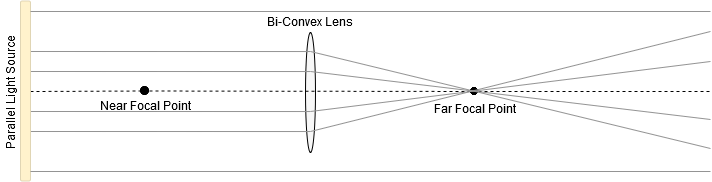
\includegraphics[width=0.8\linewidth]{figures/litreview/lens_diagram.png}
	\caption{Focal Point Illustration}
	\label{fig:lens_diagram}
\end{figure}

Figure \ref{fig:lens_diagram} above shows the near and far focal points for a lens. The diagram illustrates the behaviour of light rays produced by a theoretical parallel light source and passing through a bi-convex lens. The focal point is the common location through which parallel beams of light passing through a lens will pass. The near focal point is the apparent point location from which diverging beams produced by instead passing the parallel beams through a bi-concave lens would appear to have emanated from, should the rays be traced back along the divergent path.

In is in the interest of this investigation to consider the use of a lens to produce a beam of parallel light rays. This is essentially reversing the process illustrated in figure \ref{fig:lens_diagram}.

\begin{figure}[H]
	\centering
	\begin{minipage}{.3\textwidth}
		\centering
		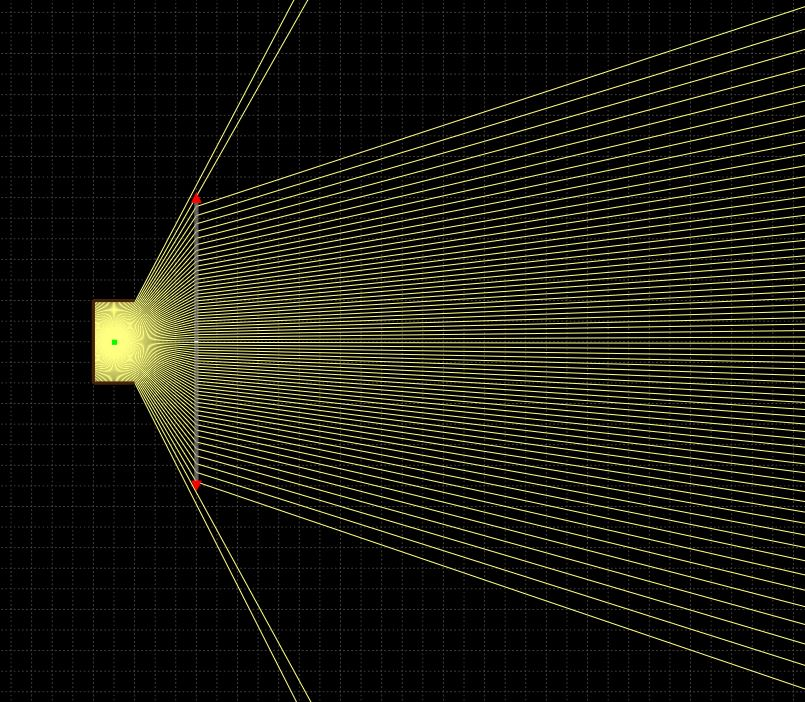
\includegraphics[width=.9\linewidth]{figures/litreview/lens_divergent_beam.JPG}
		\captionof{figure}{Divergent}
		\label{fig:lens_divergent}
	\end{minipage}%
	\begin{minipage}{.3\textwidth}
		\centering
		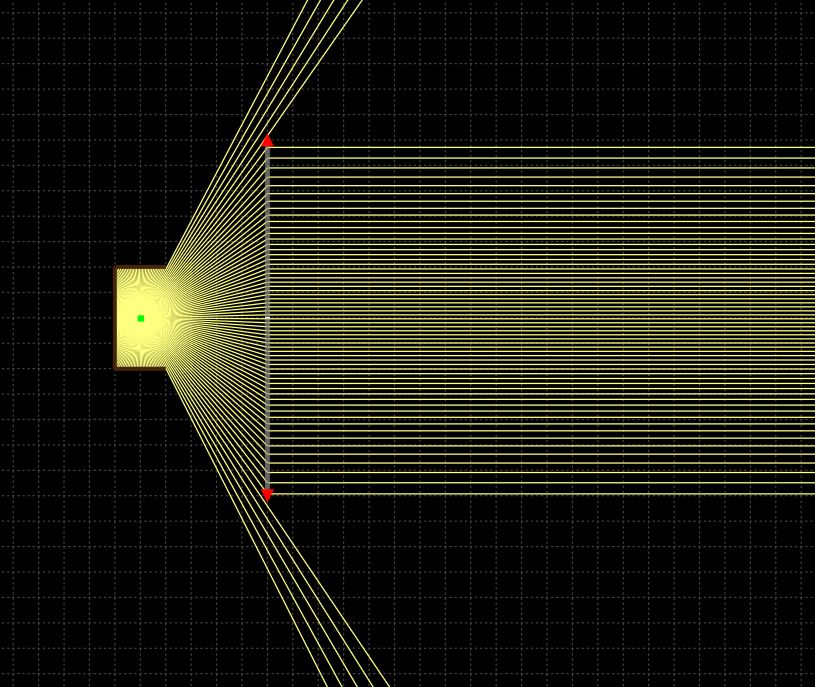
\includegraphics[width=.9\linewidth]{figures/litreview/lens_parallel_beam.JPG}
		\captionof{figure}{Parallel}
		\label{fig:lens_parallel}
	\end{minipage}
	\begin{minipage}{.3\textwidth}
		\centering
		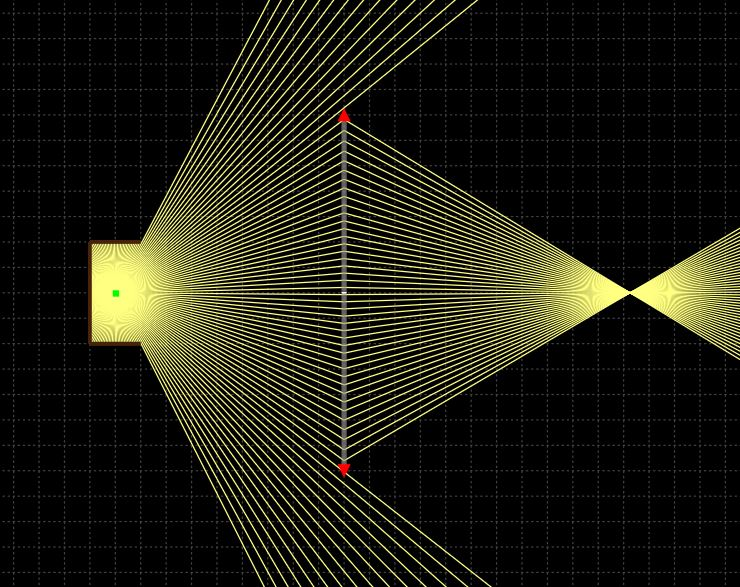
\includegraphics[width=.9\linewidth]{figures/litreview/lens_focus_beam.JPG}
		\captionof{figure}{Convergent}
		\label{fig:lens_convergent}
	\end{minipage}
	\caption*{Images showing the different behaviours of light interacting with a lens}
\end{figure}

Figures \ref{fig:lens_divergent} to \ref{fig:lens_convergent} illustrate\footnotemark the three behaviours that may be achieved using a single point source of light and an ideal lens. Behavious in figure \ref{fig:lens_divergent} occurs when a point light source exists between the near focal point and the lens, the resulting beam of light diverges after passing through the lens. Figure \ref{fig:lens_parallel} shows that for a light source placed at the focal point, the rays of light will emerge from the lens parallel. Finally \ref{fig:lens_convergent} illustrates that for a point source of light placed further beyond the near focal point (on the opposite side to the lens) results in a beam that initially converges, focusing to some point and then diverges.
\footnotetext{Created using \href{https://ricktu288.github.io/ray-optics/simulator/}{Ray-Optics Simulator}}

In may cases including this investigation, the light coming from an LED may be approximated as a point source and the lens approximated as ideal.


\subsection{IR Communication}
%This is where I talk about different IR protocols

IR has is used in many applications, this is because it is cheap, efficient and simple to use. A basic implementation can be done using an IR LED, IR receiver IC and a pair of microcontrollers.

There are several IR communication protocols in existence. Of the extensive list of available protocols the following are quite popular

\begin{itemize}
	\item RC-5
	\item RC-6
	\item NEC
	\item SIRC
\end{itemize}

Practically all the IR protocols for remote control applications follow the exact same principles for encoding and transmitting information through IR radiation. To transmit information, an IR LED is modulated at a particular carrier frequency (usually around 36kHz). Modulation is necessary because there are many sources of IR radiation and it would be otherwise impossible to distinguish the user generated IR signal from surrounding noise sources. Each protocol defines specific timing conditions for how long the IR radiation should be modulated to portray a specific symbol. This is where the various protocol differ.

Some protocols use a technique known as pulse width encoding. This technique involves modulating the IR LED for a different period of time depending on whether a 1 or 0 is to be transmitted, while maintaining a constant period of time between transmissions. This is the technique is incorporated into Sony's SIRC protocol.

Other protocols use pulse distance encoding, such as the NEC protocol by Renesas. This protocol involves modulating the IR LED for a fixed period of time and the time period between each modulation is used to indicate either a 1 or 0.

Finally, some of the IR protocols use Manchester Encoding to embed information, such as in the case of the very popular RC-5 protocol and its successor the RC-6 protocol. Due to its wide adoption and popularity \cite{rudrappa2009}, as well as incorporation of the elegant Manchester Encoding technique, it was decided to use an adaption of the RC-5 protocol in this project. A review of Manchester Encoding is detailed in section \ref{sec:manchester_encoding} below.

\subsubsection{RC-5 Protocol}
\label{sec:rc_5_protocol}
This project incorporates a modified version of the RC-5 transmission protocol. The the original RC-5 protocol is illustrated in figure \ref{fig:rc_5_protocol}. The bits are encoded using the IEEE 802.3 convention for Manchester Encoding. The modulation frequency of the carrier is 36kHz and the length of one bit period is 64 cycles or 1.778mS\cite{Perme2007}.

\begin{figure}[H]
	\centering
	
\includegraphics[width=0.8\linewidth]{figures/litreview/rc5_protocol.png}
	\caption{RC-5 IR Protocol}
	\label{fig:rc_5_protocol}
\end{figure}

Every transmission begins with two start bits, these bits always have a value of 1. Following the start bits is a 'toggle' bit. When a button is depressed, the message is transmitted repeatedly with a 114ms gap between transmissions. In remote control applications it is useful to distinguish between a button which remains depressed and a button being repeatedly pressed. This is achieved through the toggle bit which is flipped each time a button is released. Finally the RC-5 protocol first transmits a 5-bit address followed by a 6 bit command.


\subsection{Materials Interaction}
%Talk briefly about materials and the interation of different materials with IR. Mention the difficulty of aquiring these resources and therefore the exclusion of them during experiementation

%%%%%%%%%%%%%%%%%%

\section{Reliable Communication}

\subsection{Noise}
%Talk about interference and noise, sources and narrow down to IR in particular... Also note noise in components and power supplies etc.

\subsection{Modulation}
%Talk about modulation techniques 

\subsection{Manchester Encoding}
\label{sec:manchester_encoding}
Manchester Code is a type of phase encoding. It is classified as a line code and is produced by generating patterns through some measurable phenomena. The commonly used mediums to represent a Manchester encoded signal would be voltage, current and light (electromagnetic radiation).

Manchester coding, as its name suggests, was developed at the University of Manchester and it was first published in 1949 \cite{Jameel2019}. Manchester encoding is a protocol for integrating the clock and data into a single sequence consisting of only two symbols. It does not require clock synchronization, only that a predefined bit-width is known by both the receiver and transmitter. 

The principle behind Manchester code is to encode the information into transitions between two symbols. This technique makes the encoding scheme particularly useful in communication by means of inductive coupling such as in RFID. Due to its self-clocking property and simplicity it is the standard means of encoding for many IR applications. Perhaps the most common application is in the remote controls we use for various appliances.

Manchester code is a special form of binary phase shift keying (BPSK). A square wave of a particular frequency is chosen as the carrier and binary information is encoding by adjusting the setting a phase off set to either 0\degree or 180\degree s. In figure \ref{fig:manchesterencoding} the process of encoding 10 bits is illustrated. Two conventions exist, their difference lies solely in the definition of which logic values are represented by each of the two transitions. The convention used throughout this investigation is in accordance to the IEEE 802.3 standard which defines a logical 1 as the transition from 0 to 1 and a zero as 1 to 0. The other convention used by inventor G.E. Thomas is the inverse of this and is also widely used.\\

\begin{figure}[H]
	\centering
	
\includegraphics[width=0.7\linewidth]{figures/litreview/manchester_encoding}
	\caption{Manchester code example using 10 bits}
	\label{fig:manchesterencoding}
\end{figure}

\subsubsection{Encoding Algorithm}

%here breifly go over the simple manchester encoding tecnique


\subsubsection{Decoding Algorithm}
Different techniques have been developed to decode Manchester encoded sequences. In his paper on methods for decoding Manchester code, R. A. Dobre discusses an elegant and widely used finite state machine approach which has been illustrated in figure \ref{fig:manchesterdecodingfsm} below. \cite{Dobre2014}

\begin{figure}[H]
	\centering
	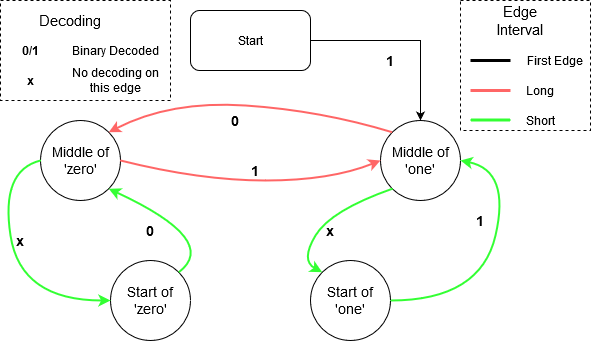
\includegraphics[width=0.7\linewidth]{figures/litreview/manchester_decoding_fsm.png}
	\caption{FSM Algorithm for Decoding Manchester Sequences}
	\label{fig:manchesterdecodingfsm}
\end{figure}

The state machine approach is particularly useful because it only considers the time period between the current detected edge and the previous edge. It removes the need to track samples saving on memory and reducing processing power requirements, all without introducing additional complexity.

It should be noted that this FSM assumes the first bit transmitted is always a logical 1. In addition does not detect the end of a sequence, so additional logic is required such as a counter to detect when a certain number of bits have been received or by means of implementing timeout detection.

%\iffalse
\subsection{Error Control}

In information theory, error control is the field of study that concerns issues of detecting errors in digital communications and in certain instances provides the means to corrected these errors. Whenever data is transmitted over some kind of network, there is the possibility that interference can cause a bit to flip resulting in an error. Richard Hamming pioneered in the development of digital error control and is known for (amongst other things) the Hamming code.

Various ways to detect and potentially correct the presence of an error. The most trivial technique known as a 'repetition code' simply involves sending the information three times, making it possible to detect if one of the three data-streams doesn't match the others. Although repetition codes allows for both error detection and correction, it is horribly inefficient. Various techniques have been developed and each technique balances complexity and efficiency.

\subsubsection{Parity}
Using a parity bit is the most simple means to detect an error in a bit sequence. The parity of a sequence may be defined as the result of a bit wise exclusive or (XOR) operation, this is known as 'even parity' because the parity bit value is chosen such that upon appending it to the bit-sequence there would be an even number of 1s. Conversely 'odd parity' calculates the parity bit such the number of 1s in the generated sequence is odd. Table \ref{tbl:party_examples} below provides example bit sequences and the respective even (given by the XOR operation) and odd parity values.

\begin{table}[H]
	\centering
	\begin{tabular}{ccc}
		\hline
		\multicolumn{1}{l}{\textbf{Bit Sequence}} & \textbf{XOR of Bits} & \multicolumn{1}{l}{\textbf{Odd Parity Bit}} \\ \hline
		0000000 & 0 & 1 \\ \hline
		1111111 & 1 & 0 \\ \hline
		1010101 & 0 & 1 \\ \hline
		1001100 & 1 & 0 \\ \hline
	\end{tabular}
	\caption{Even and odd parity for example bit sequences}
	\label{tbl:party_examples}
\end{table}

 To use parity as a method to detect errors, the sender and receiver choose to use either even or odd parity. Before transmission, the sender calculates the parity bit for the sequence to be sent, this bit is then appended to the bit-stream. Upon receiving the bit-stream, the same parity calculation is done on the sequence. If the result of this calculation is a 1 it can be said for certain that an error occurred, if the result is zero it can be said that no error occurred or an even number of errors occurred.

%\subsubsection{Hamming Code}

%\fi


\subsection{Demodulation}
%Give an overview of demodulating and what techniques exist: Goertzel, DFT, tone-detectors, next sections hilights details


%%%%%%%%%%%%%%%%%%
\section{Digital Signal Processing}
In the age of micro-controllers and micro-processors, in many situations it has become far more effective to use digital signal processing to manipulate and processes signals.

Part of the IR decoding process requires detecting the presence of a particular frequency (commonly referred to as a tone). The natural tool to turn to when examining the frequency content of a signal is the discrete Fourier transform (DFT). The DFT is well established and there exist a variety of algorithms which compute its values, perhaps the most well known being the FFT. However, for the purposes of detecting a single tone of a predetermined frequency, the DFT is not the most efficient method, even when optimized algorithms such as the FFT are implemented.

The FFT provides a very efficient means for determining all the DFT coefficients, but in a use case only a few of the coefficients are used and the rest discarded it is not the most efficient technique. By using a less efficient process for calculating individual coefficients of the DFT it is possible to greatly reduce program complexity and processing time relative to an implementation that uses the FFT.

\subsection{Goertzel Algorithm}

The algorithm which computes individual DFT coefficients is known as the Goertzel algorithm (or Goertzel Filter) and was developed by G. Goertzel in 1958. \cite{Goertzel1958} A common application of the Goertzel algorithm is in the decoding of DTMF\footnotemark{} signals.
\footnotetext{Duel Tone Multiple Frequency}

\subsubsection{Derivation}
The goertzel algorithm may be derived from the formula for the DFT. In the derivation \(W_N = e^{-j\frac{2\pi}{N}}\).

\begin{equation}
	\label{eqn:dft_defn}
	X[k] = \sum_{n=0}^{N-1}x[n]W_{N}^{nk}
\end{equation}

Multipling the right side of equation \ref{eqn:dft_defn} by \(W_{N}^{-Nk} = e^{j\frac{2\pi N k}{N}} = 1\) we get

\begin{equation}
X[k] = W_{N}^{-Nk}\sum_{n=0}^{N-1}x[n]W_{N}^{nk}
\end{equation}

Rearranging we get

\begin{equation}
\label{eqn:dft_conv}
X[k] = \sum_{n=0}^{N-1}x[n]W_{N}^{k(n-N)}
\end{equation}

Notice that if we consider the signal \(h_k[l] = W_N^{-kl}u[l]\), then equation \ref{eqn:dft_conv} is the convolution of $h_k[l]$ with $x[l]$. Substituting these signals into equation \ref{eqn:dconv} (formula for discrete convolution) below, we can rearrange the result to arrive at equation \ref{eqn:dconv_sub}.

\begin{equation}
	\label{eqn:dconv}
	y_k[l] = \sum_{m=0}^{N-1}x[m]h_k[l - m]
\end{equation}

\begin{equation}
	\label{eqn:dconv_sub}
y_k[l] = \sum_{m=0}^{N-1}x[m]W_N^{k(m-l)}
\end{equation}

Comparing equation \ref{eqn:dft_conv} with equation \ref{eqn:dconv_sub}, it becomes clear that from the convolution $y_k[n] = x[n] * h_k[n]$ we can find the value of $X[k]$ by substituding N into $y_k[n]$. Thus the following relationship exists

\begin{equation}
\label{eqn:goertzel_relationship}
X[k] = y_k[N]
\end{equation}

%%%%
%Now deriving the filter
%%%%

In their paper on generalizing the Goertzel algorithm for non-integer multiples of the the fundamental frequency, P. Sysel and P. Rajmic show how the function $h_k[n]$ may be transformed to the Z-domain and optimized to reduce the amount of computational power required to compute the DFT coefficient \cite{Sysel2012}. The results are given by the following equations.

%The following equations are taken from the paper - check if thats okay with Simon...
\[h_k[n] \xRightarrow{\text{Z}} H_k(z)\]

\begin{equation}
W_N^{-kl}u[n] \xRightarrow{\text{Z}} \frac{1}{1 - W_N^{-k}z^{-1}} = \frac{1}{1 - e^{j\frac{2\pi k}{N}}z^{-1}}
\end{equation}

$H_k(z)$ can then be manipulated to give

\begin{equation}
\label{eqn:g_optimized_ir}
H_k(z) = \frac{1 - e^{-j\frac{2\pi k}{N}}z^{-1}}{1 - 2cos(\frac{2\pi k}{N})z^{-1} + z^{-2}}
\end{equation}

Finally, equation \ref{eqn:g_optimized_ir} can be converted to state variable form to yeild the following


\begin{equation}
	\label{eqn:g_ss}
	s[n] = x[n]+2cos(\frac{2\pi k}{N})s[n-1]-s[n-2]
\end{equation}


\begin{equation}
	\label{eqn:g_ssoutput}
	y_k[n] = s[n]-e^{-j\frac{2\pi k}{N}}s[n-1]
\end{equation}



\subsubsection{Implementation}
\label{sec:goertzel_implementation}
Using the state variable equations \ref{eqn:g_ss} and \ref{eqn:g_ssoutput} we can implement the goertzel filter digitally. The following code in listing \ref{lst:goertzel_algorithm} shows a Goertzel filter implemented in the Octave environment.

\begin{lstlisting}[caption={Goertzel Algorithm - Octave Implementation\label{lst:goertzel_algorithm}}]
function magnitudesqd = calculate_goertzel (N, bin_frequency, sampling_frequency, samples)

	k = round(N*bin_frequency/sampling_frequency);
	omega = (2*pi*k)/N;
	cosval = cos(omega);
	sinval = sin(omega);
	coeff = 2*cosval;
	
	s1 = 0;
	s2 = 0;
	
	for i = 1:N
	s0 = (samples(i) + (coeff*s1) - s2);
	s2 = s1;
	s1 = s0;    
	end
	
	realv = (s1 - (s2 * cosval));
	imgv = (s2 * sinval);  
	
	magnitudesqd = realv*realv + imgv*imgv;

endfunction
\end{lstlisting}

\subsubsection{Nyquist-Shannon}

\[f_{Nyquist} = \frac{f_{sampling}}{2}\]

\begin{equation}
\label{eqn:sampling_frequency}
BW < f_{Nyquist}
\end{equation}


\subsubsection{Anti-alias Filtering}
%todo: chat a bit about designing an anti-aliassing filter



%%%%%%%%%%%%%%%%%%

\section{IR Radiation}
This is where I talk about the section of the EM spectrum that is IR


\subsection{IR Radiation Detection}

%Explain how photodiodes and phototransistors work




\section{TALK ABOUT}
\begin{itemize}
	\item Automatic gain control (and why it was excluded - time, cost and computational power)
	\item Hamming Codes (and why it was excluded)
\end{itemize}








\chapter{Methodology}
\label{ch_methodology}

\section{Outline}

This study is an investigation into the performance of modules which form a uni-directional data link for use in laser tag systems. The following chapter presents the methodology that was followed throughout the investigation. A phased approach was taken and has been illustrated in figure \ref{fig:methodology_overview}.

\subsubsection{Phases Overview}
The first phase constitutes a survey of the relevant literature. During the second phase, the identification and design of the modular subsystems take place. This is followed by the third phase during which the modules are implemented according to their design.

In following the design paradigm of the spiral model, a feedback path from the development and realization stage back to the system design phase was incorporated. This was done to allow new information learned during the third phase to be incorporated into the system design.

\begin{figure}[H]
	\centering
	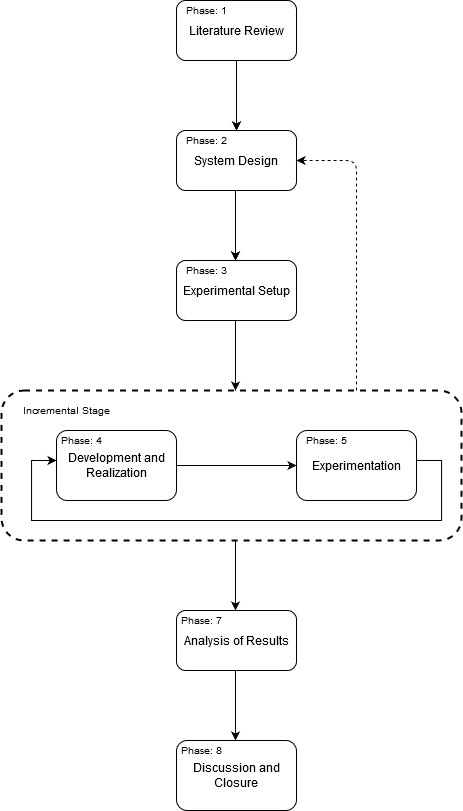
\includegraphics[width=0.5\textwidth]{figures/methodology/methodology}
	\caption{Methodology Flow Diagram}
	\label{fig:methodology_overview}
\end{figure}

Following the development and realization phase is an iterative stage which encapsulates both the experimental setup (phase 4) and the experimentation (phase 5).

During the seventh phase of the investigation, the results are analysed and observations are recorded. The eighth phase concludes the investigation with a final discussion and closing remarks.


\section{Phase 1 - Literature}

During the first phase of the project, the relevant literature is reviewed. The objective of this phase is to determine the various techniques that have been established in the field of optical communication. For each of the topics, a broad overview is presented, followed by a detailed review of specific concepts and theories.

The design and evaluation of a complex communication system involve reviewing theory in various areas and the following questions served as a guide for surveying the available literature.

\begin{itemize}
	\item How might light be manipulated into a narrow beam? %Optics
	\item How do light-based communication systems function? %Optical comms
	\item What methods exist for electronically sensing of light? %Detection of Radiation
	\item What techniques are appropriate for reliable communication? %Reliable Communication
	\item What techniques are appropriate for signal processing? %DSP &Analog processing
\end{itemize}

The literature review is presented in chapter \ref{ch_literature}.

%%%%%%%%%%%%%%%%%%%%

\section{Phase 2 - Design}

The design phase of this investigation is dedicated to the development of individual modules and software algorithms. This phase begins with a decomposition of the uni-directional communication system into a set of modules. Figure \ref{fig:designoverview} provides a high-level overview of the system decomposition.

\begin{figure}[H]
	\centering
	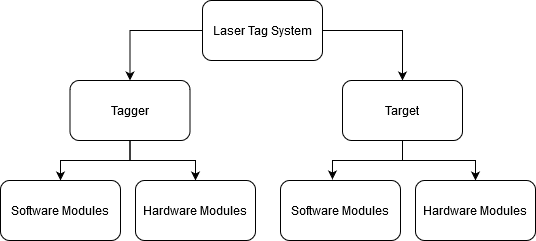
\includegraphics[width=0.7\linewidth]{figures/methodology/design_overview}
	\caption{Design Overview}
	\label{fig:designoverview}
\end{figure}

The second phase is documented in chapter \ref{ch_design}. For each module, a brief description of the purpose and required functionality of the module is given. The design of the module is then presented, including important calculations, circuit schematics and relevant diagrams where appropriate. For each module, an image of the final implementation is also shown.

Throughout the design phase, various simulations were used to predict the behaviour of algorithms\footnote{Octave was used to validate algorithms} and circuits\footnote{LTSpice was used to simulate circuits}.

%%%%%%%%%%%%%%%%%%%%

\section{Phase 3 - Development and Realization}

The third phase concerns the development of the individual modules. During this phase, each module was realized according to its design.

Modules were first implemented on a breadboard to confirm valid behaviour. In the case of a failed implementation due to a design oversight the design was reworked, this is illustrated using a dotted feedback path from phase 3 to phase 2 in figure \ref{fig:methodology_overview}. Only the final designs and implementations have been documented in the body of this report.

Except for the STM32 development boards, all the module designs were implemented on strip-board. The use of PCBs was avoided due to uncertainty caused by the COVID-19 epidemic.

%%%%%%%%%%%%%%%%%%%%


\section{Phase 4 - Experimental Setup}

The fourth phase is the experimental set-up. This phase outlines the procedure followed to set up the test and measurement equipment and the module or collection of modules to perform experiments and gather empirical data. Chapter \ref{ch_experimentation} is dedicated to the procedures followed for each experiment.

Due to the unique functionality of each module, it is necessary to use different experimental setups to evaluate different modules. Hence phase four forms part of an iterative stage which is used to illustrate that for various phases of experimentation, a unique experimental setup has been devised.

Equipment used throughout this investigation is documented at the end of this chapter in section \ref{sec:test_and_measurement_equipment}


%%%%%%%%%%%%%%%%%%%%



\section{Phase 5 - Experimentation}

Phase five concerns the execution of the experiments outlined in chapter \ref{ch_experimentation} and forms the second half of the iterative stage. During this phase, the experiments are executed and the results are prepared for analysis.

The objective of the experimentation phase is to provide results that may be used to gain insight into each module's performance. Results will consist primarily of empirical results, but in certain cases also include simulation results.

The results gathered during the experimentation phase are documented in chapter \ref{ch_results}.

%%%%%%%%%%%%%%%%%%%%

\section{Phase 7 - Analysis of Results}

The seventh phase of this investigation is the analysis of results gathered during the experimentation. The objective of this phase is to interpret the results and draw insights.

During this phase, the performance of the individual modules is evaluated. Brief reasoning is provided where the results do not align with the theorised outcome.

To increase the readability of this report, the analysis of the results has been recorded in the results chapter. For each experiment, the analysis is presented directly below the results, under the heading 'discussion'.

%%%%%%%%%%%%%%%%%%%%

\section{Phase 8 - Discussion and Closure}

In this final phase of the project, the results and analysis of the results are discussed in the greater context of the problems being investigated. The discussion will comment on the effectiveness of each of the modules. 

Discussion is bought to a close with recommendations for further research.


%%%%%%%%%%%%%%%%%%%%

\section{Equipment}
\label{sec:test_and_measurement_equipment}
The following section outlines the equipment used during the development phase as well as test and measurement phase of the project.

\subsubsection{Oscilloscope and Function Generator}
To perform electrical measurements, the Picoscope 2205A by Pico Technology was used. The Picoscope has two input channels and a dedicated function generator. The function generator was used to inject waveforms in various experiments.

\subsubsection{Microcontroller Development}
The CubeIDE developer environment by STMicroelectronics was used to develop the firmware for the tagger, target and tone decoder's central processor.

\subsubsection{Signal Processing and Data Presentation}
The Octave mathematical programming language was used to develop and predict the behaviour of the digital signal processing algorithm as well as generate plots of the data collected in various experiments.

\subsubsection{Serial Communication}
Serial communication with the STM32 microcontrollers was handled by Realterm \footnote{\url{https://sourceforge.net/projects/realterm/}}, a free serial monitor available for Windows.

\subsubsection{Circuit Simulation}
The LTSpice SPICE simulation environment by Linear Technology\footnote{LT corporation is owned by Analog Devices} was used to test and develop the circuit modules.

\subsubsection{Test and Measurement}
For general purpose measurements of voltages, current and resistance the Fragram T2612 digital multimeter was used.

The Sony Handycam DCR-HC26 video camera was used to \textit{see} the invisible beam spot produced by the LED focus system.

A digital calliper was used to perform measurements less than 300mm, measurements longer than 300mm were taken using a measuring tape.





\chapter{Design}
\label{ch_design}

This chapter is dedicated to the various modules which comprise the laser tag system being investigated. The system is complex and comprises of many modules both in hardware and software. An overview of the entire system is given followed by the design of the individual modules.

The system overview covers the two main subsystems, the tagger subsystem and target subsystem. Following the system overview these two subsystems are divided into modules and categorized into either hardware or software. The design of each module is presented, along with an image of the final implementation.

%todo: possibly explain why designs are so ellaborate... This investigation is centred on the creation and evaluation of system modules, therefore the design descriptions have been written 

%todo: give an explaination as to how the module design has been brocken down into subsubsections

\section{System Overview}

Figure \ref{fig:system_overview_hardware} gives an overview of the modules that make up the laser tag data link system.

\begin{figure}[H]
	\centering
	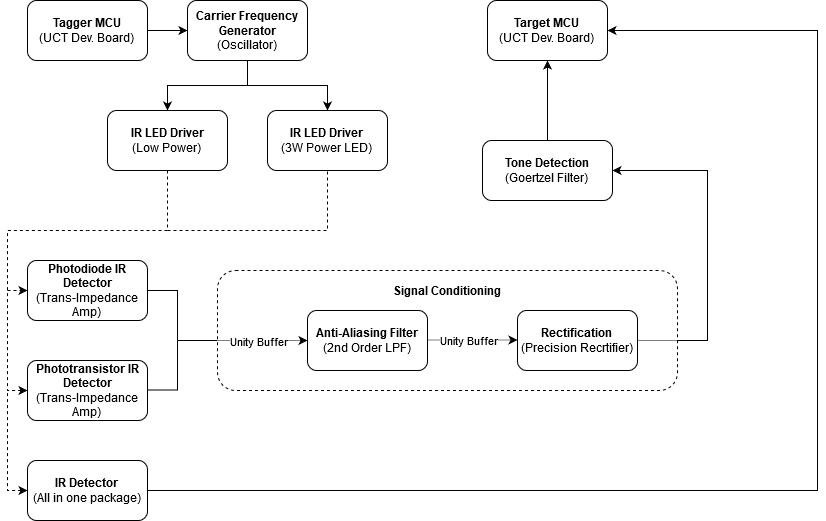
\includegraphics[width=0.9\textwidth]{figures/design/system_overview_hardware}
	\caption{Block Diagram of Hardware Modules}
	\label{fig:system_overview_hardware}
\end{figure}

\subsection{Subsystems}

Two subsystems may be derived from figure \ref{fig:system_overview_hardware}. The tagger subsystem responsible for generating and transmitting a message and the target subsystem responsible for receiving and decoding an incoming message.

\subsubsection{Tagger Subsystem}
The tagger subsystem comprises a main processor, carrier frequency generation module and two LED driver modules. For the purposes of this investigation the UCT STM32\footnotemark{} development board has been used as the main processor. The development board communicates with the carrier frequency generation module (responsible for producing the 36kHz square waveform), this module is connected to an LED driver module which in turn drives an IR LED. Two led driver modules have been design and both operate on the same input signal. The difference between the two modules is in the rated output power, the low power module is designed to drive a standard low power IR led while the high power module has been designed to drive a high power 3W IR led.

Not shown on the system overview is the light focus hardware module. This module is a passive optical component designed to focus the IR light.

\footnotetext{STM32F051C6}

\subsubsection{Target Subsystem}
The target system comprises more modules than the tagger due to the comparably higher complexity involved in detecting and processing incoming signals. The first stage of this subsystem concerns detecting incoming IR light, three different modules have been designed to perform this operation to allow for comparison between these separate approaches. As outlined in the overview shown in figure \ref{fig:system_overview_hardware} the IR receiver demodulates the detected IR light directly, however the remaining two detectors required additional modules to condition and demodulate the Manchester sequence.

These additional modules perform anti-alias filtering and rectification of the signal as well as indicate when a 36kHz tone is present in the conditioned signal. This tone detection is performed by a digital signal processing (DSP) algorithm and is implemented on the STM32 MPU.

The final module of the target subsystem is the main processor which is implemented on a second UCT STM32 development board.

\subsubsection{Software}

There are three main software components to the overall system.
\begin{itemize}
	\item The software operating on the tagger main processor used to encode and produce the Manchester data sequence.
	\item The software responsible for receiving and decoding the Manchester sequence on the target main processor.
	\item  The DSP algorithm operating on the tone detection module.
\end{itemize}


\section{Hardware Design}

\subsection{Tagger \& Target MCUs}
%Missing
% - Schematic and the like in the appendix
The laser tag systems has two main processors. One for the tagger and another for the target. The hardware used for main processor in each case is the UCT development board built around the STM32F051C6 microcontroller.

\begin{figure}[H]
	\centering
	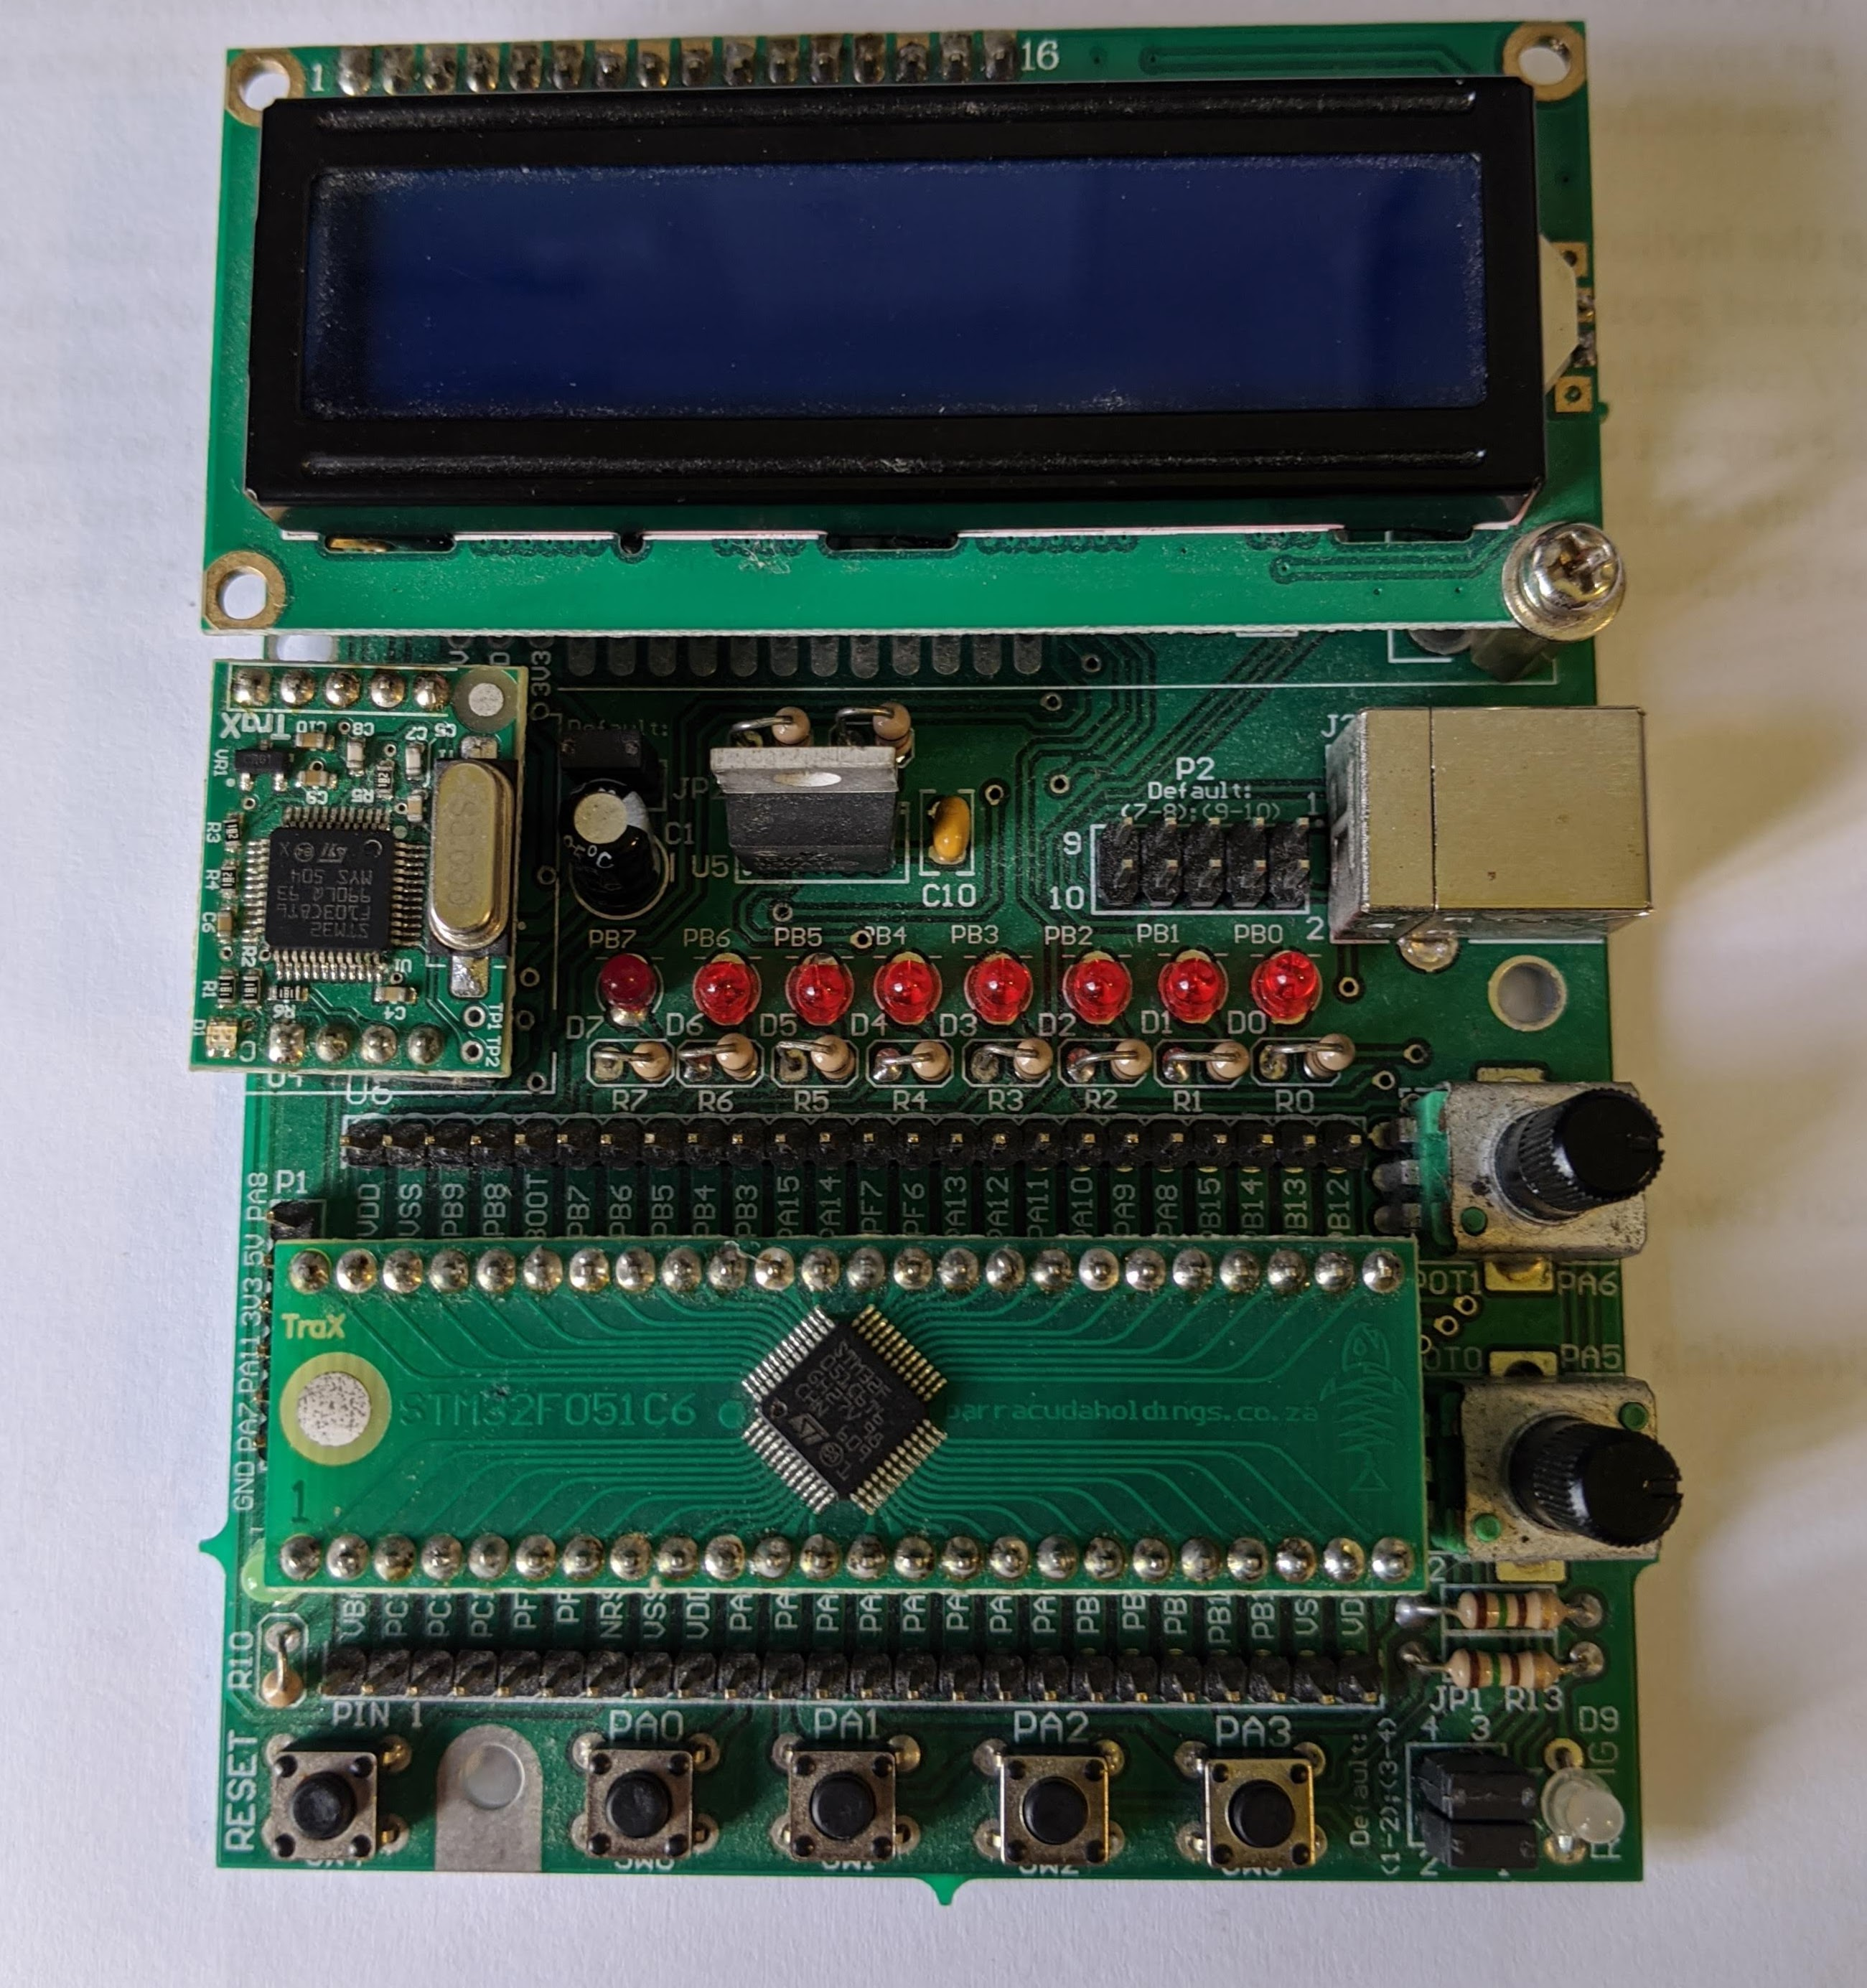
\includegraphics[width=.5\textwidth]{figures/design/dev_board_image.jpg}
	\caption{UCT STM32 Development Board}
	\label{fig:stm32_dev_board}
\end{figure}

The development board provides break-out pins for the microcontroller, 4 input buttons, an array of 8 LEDs, an LCD display and a built-in st-link v2 for debugging and programming the processor.

The STM32F051C6 was chosen partly because of its integration into the UCT development board making it easily obtainable at a low price and because of the following features

\begin{itemize}
	\item Analog to digital converter (ADC) peripheral
	\item Direct memory access (DMA) peripheral
	\item Timer peripherals with multiple interrupt channels
	\item Nested vectored interrupt controller (NVIC)
\end{itemize}



%%%%%%%%%%%%%%%%%%%%%%%%%%%%%%%%%%%%%%%%%%%%%%%%%%%%%%%%%%%



\subsection{Carrier Frequency Generator}
%Missing
% - Calculations and chosen values
\subsubsection{Functional Design}
To generate the 36kHz carrier waveform the LM555 timer IC was used. The module is designed to receive a 3.3V control signal. When a high logic level is received, the module switches the output at 36kHz to produce a square waveform.

The LED driver modules designed to be controlled by an open-collector, therefore a transistor was used to convert the push-pull output of the 555 timer to an open-collector output.

The 555 timer operates on the 5V supply connected to the module, therefore transistors were used to convert the 3.3V control signal to a 5V input for the RST pin.

\subsubsection{Schematic}
Figure \ref{fig:schematic_carrier_generation} below shows the schematic for the module.

\begin{figure}[H]
	\centering
	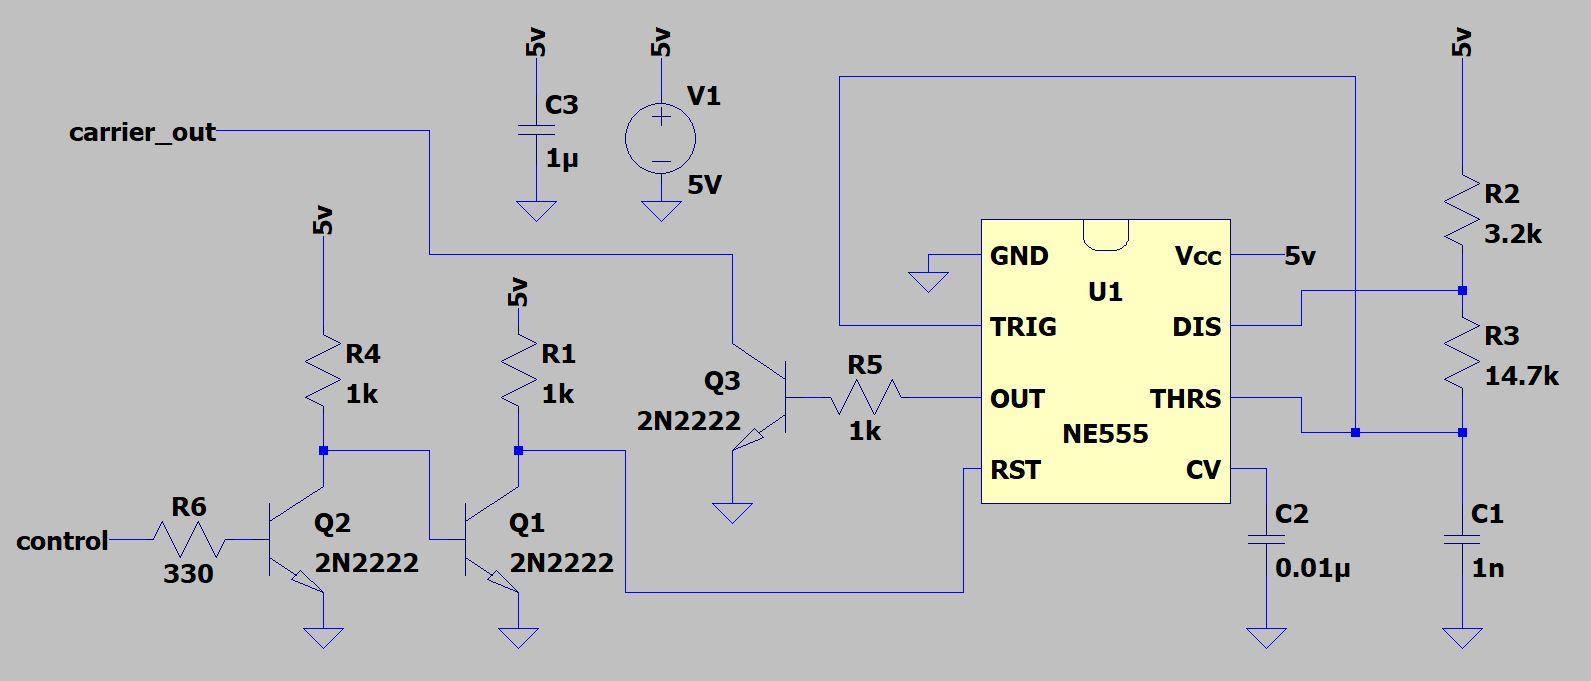
\includegraphics[width=.8\textwidth]{figures/design/carrier_waveform_generator_555.JPG}
	\caption{Carrier Generation Module Schematic}
	\label{fig:schematic_carrier_generation}
\end{figure}

\subsubsection{Frequency Generation}
%todo: this needs to be completed

According to the data sheet the period my be calculated as \(T = 0.693 (R_2 + 2R_3) C1\). A capacitor value of 10nF was chosen. Therefore, to generate a waveform with the desired period of $27.7\mu S$ the required theoretical value of $(R_2 + 2R_3)$ is $4k\Omega$.
%todo: finnish explaining resistor choice

%todo: finnish this paragraph
%After testing
The above design was implemented on a breadboard to test the

\subsubsection{Module Realization}
The strip-board implementation of the module is shown in figure \ref{fig:module_carrier_generation} below.

\begin{figure}[H]
	\centering
	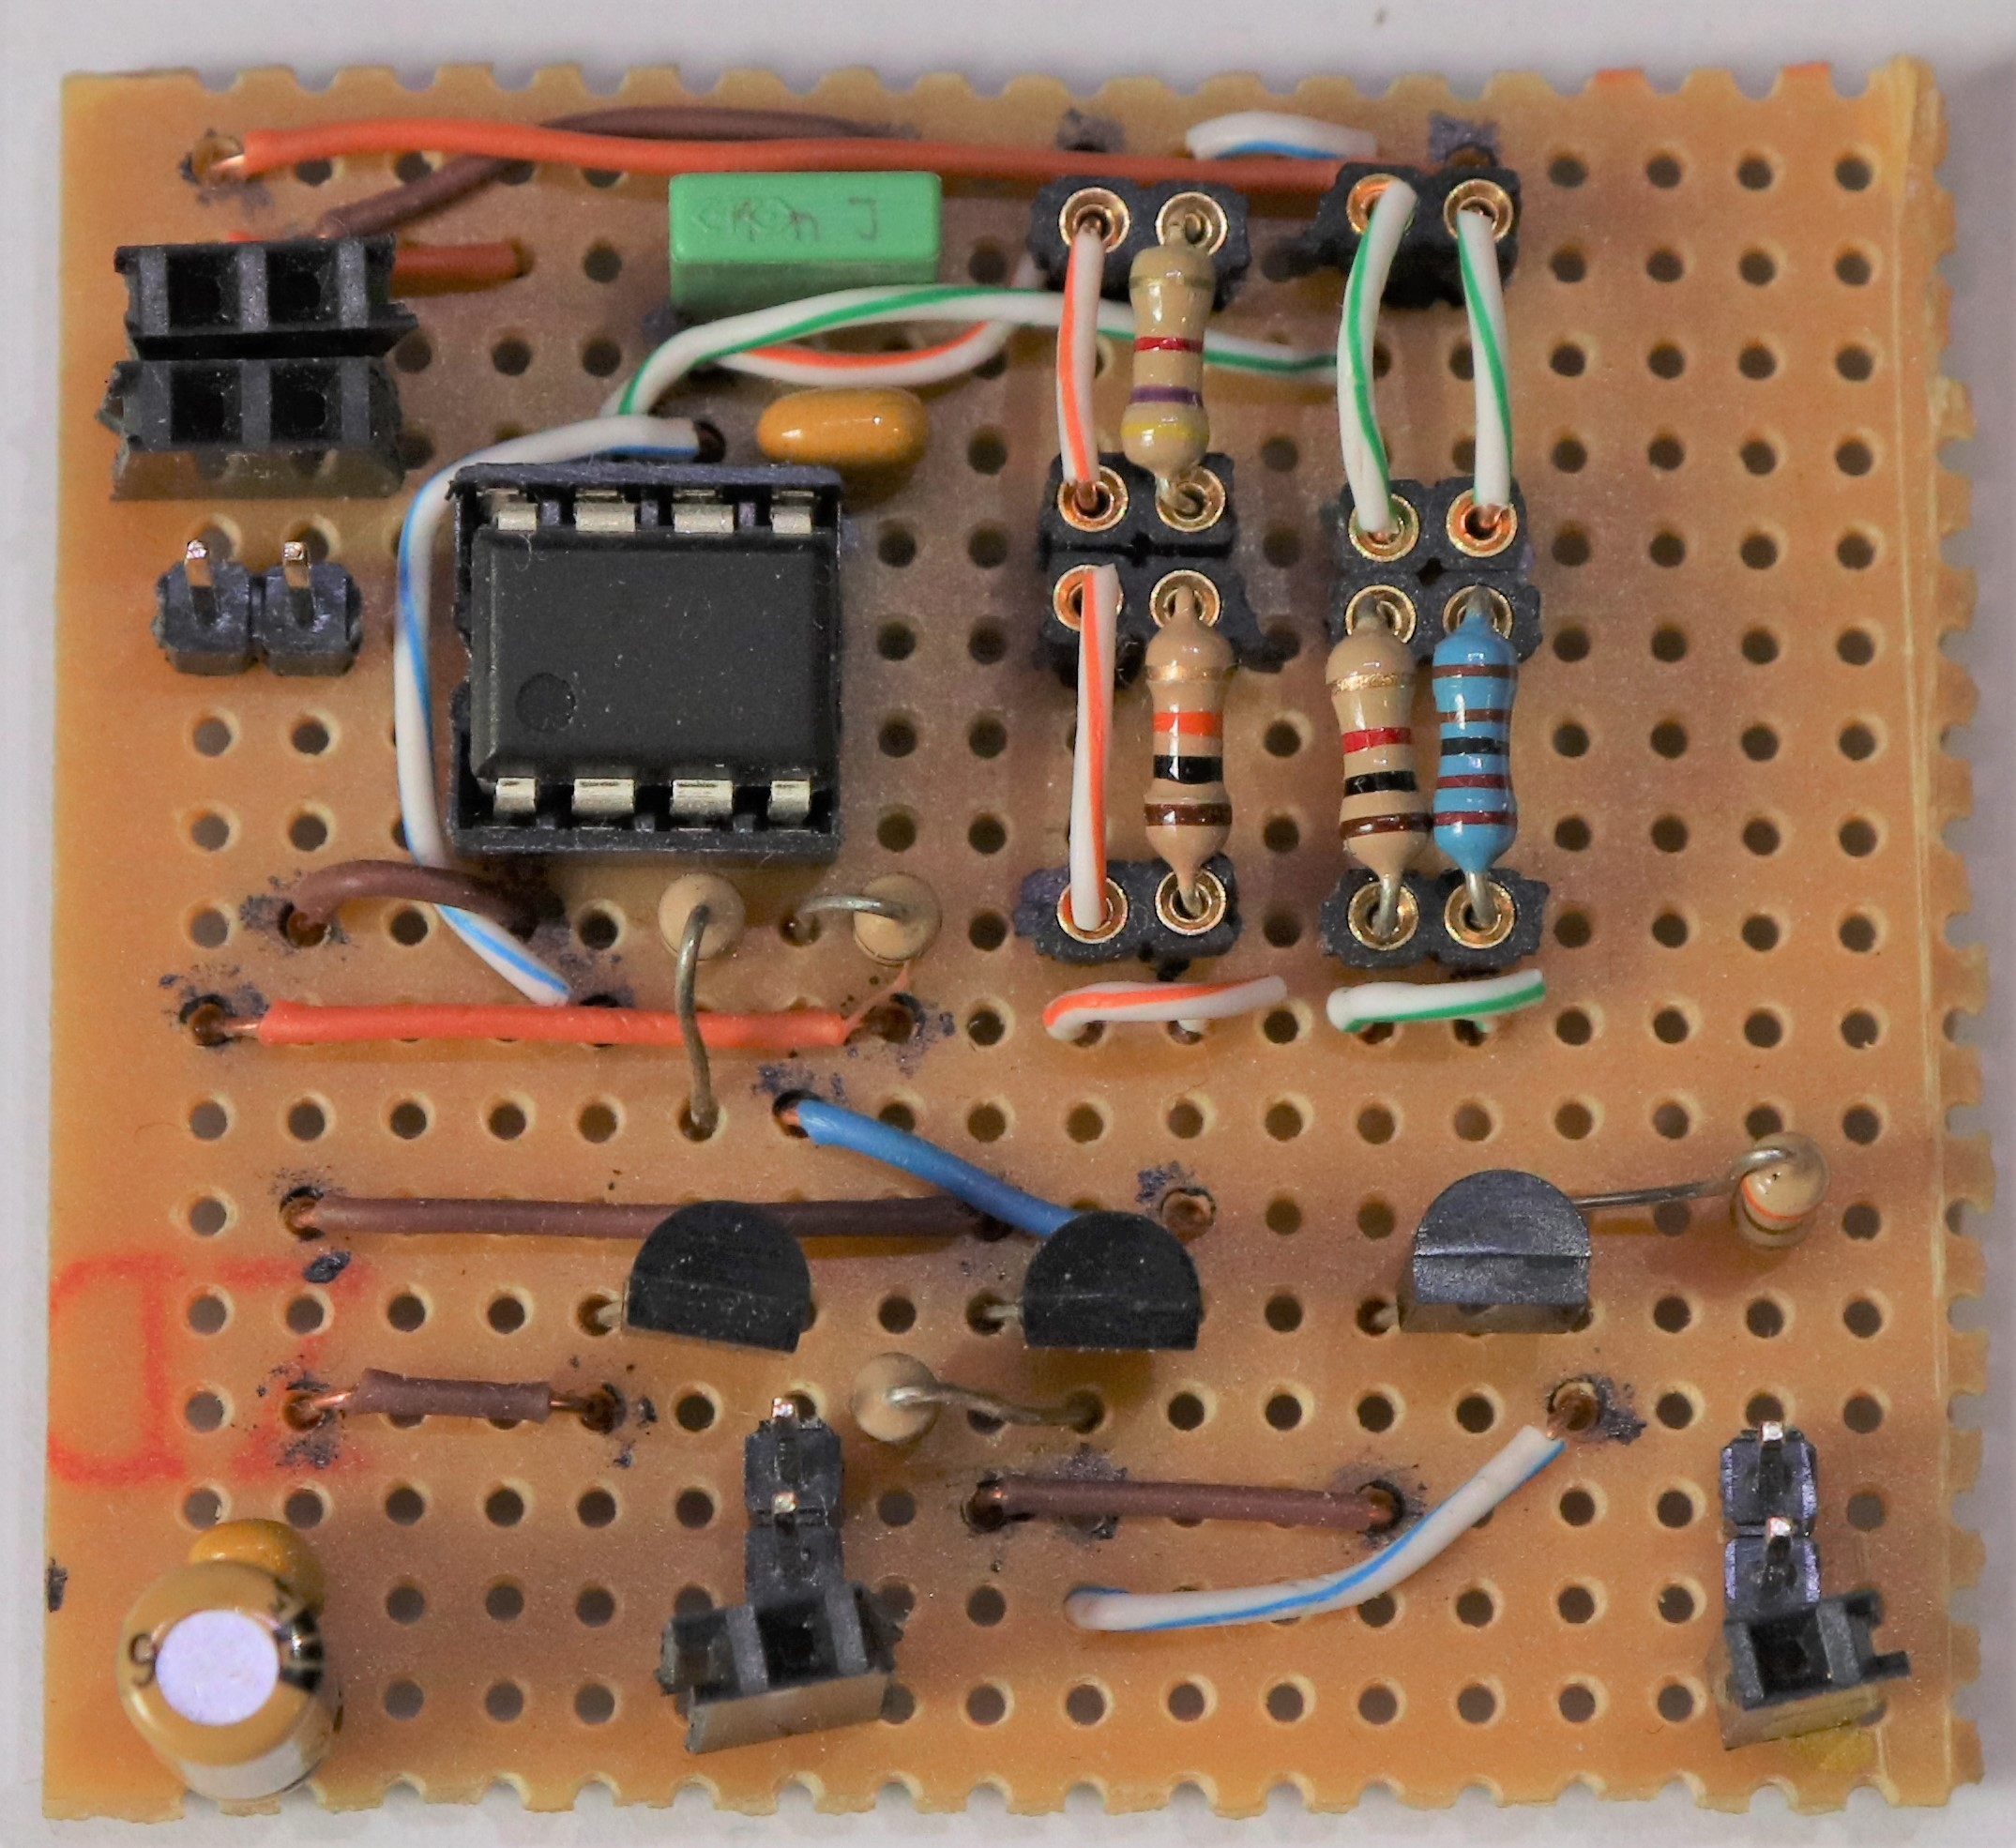
\includegraphics[width=.6\textwidth]{figures/modules/carrier_generator.jpg}
	\caption{Carrier Generation Module}
	\label{fig:module_carrier_generation}
\end{figure}



%%%%%%%%%%%%%%%%%%%%%%%%%%%%%%%%%%%%%%%%%%%%%%%%%%%%%%%%%%%



\subsection{Power LED Driver}

\subsubsection{Functional Design}
To operate the 3W high power IR LED a constant current driver module needed to be implemented. The module is designed to be controlled by an open-collector control signal such that when the control signal is pulled low the led is illuminated. The output of this module is a constant current designed to drive a power LED.

\subsubsection{Schematic}
Figure \ref{fig:schematic_power_led_driver} shows the design of a high power linear regulator, built around the IRLZ44 enhancement PMOSFET. Heat-sinks where attached to both the high power LED and the IRLZ44 power MOSFET.

\begin{figure}[H]
	\centering
	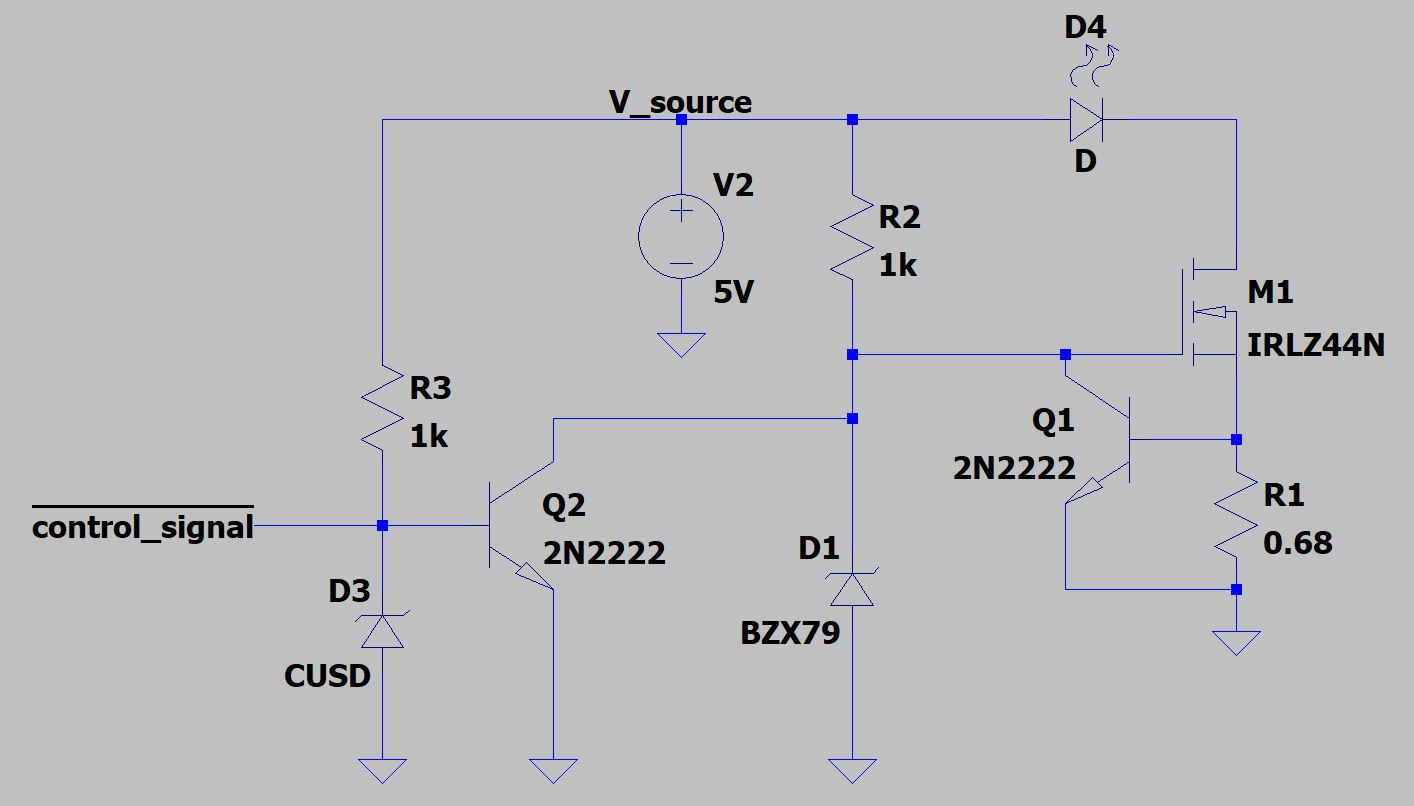
\includegraphics[width=.8\textwidth]{figures/design/power_led_driver.JPG}
	\caption{Power LED Driver Module Schematic}
	\label{fig:schematic_power_led_driver}
\end{figure}

\subsubsection{Constant Current Control}
%todo: Specs and component choice etc.

Because the LED needs to be modulated at 36kHz, standard LED driver ICs that use a switching regulator are not viable. This is because the switching frequency used in commonly available constant current switching regulators is not high enough. Instead a linear regulator was designed using discrete components.

%todo: explain how the circuit works


\subsubsection{Module Realization}
The strip-board implementation of the module is shown in figure \ref{fig:module_power_led_driver} below.

\begin{figure}[H]
	\centering
	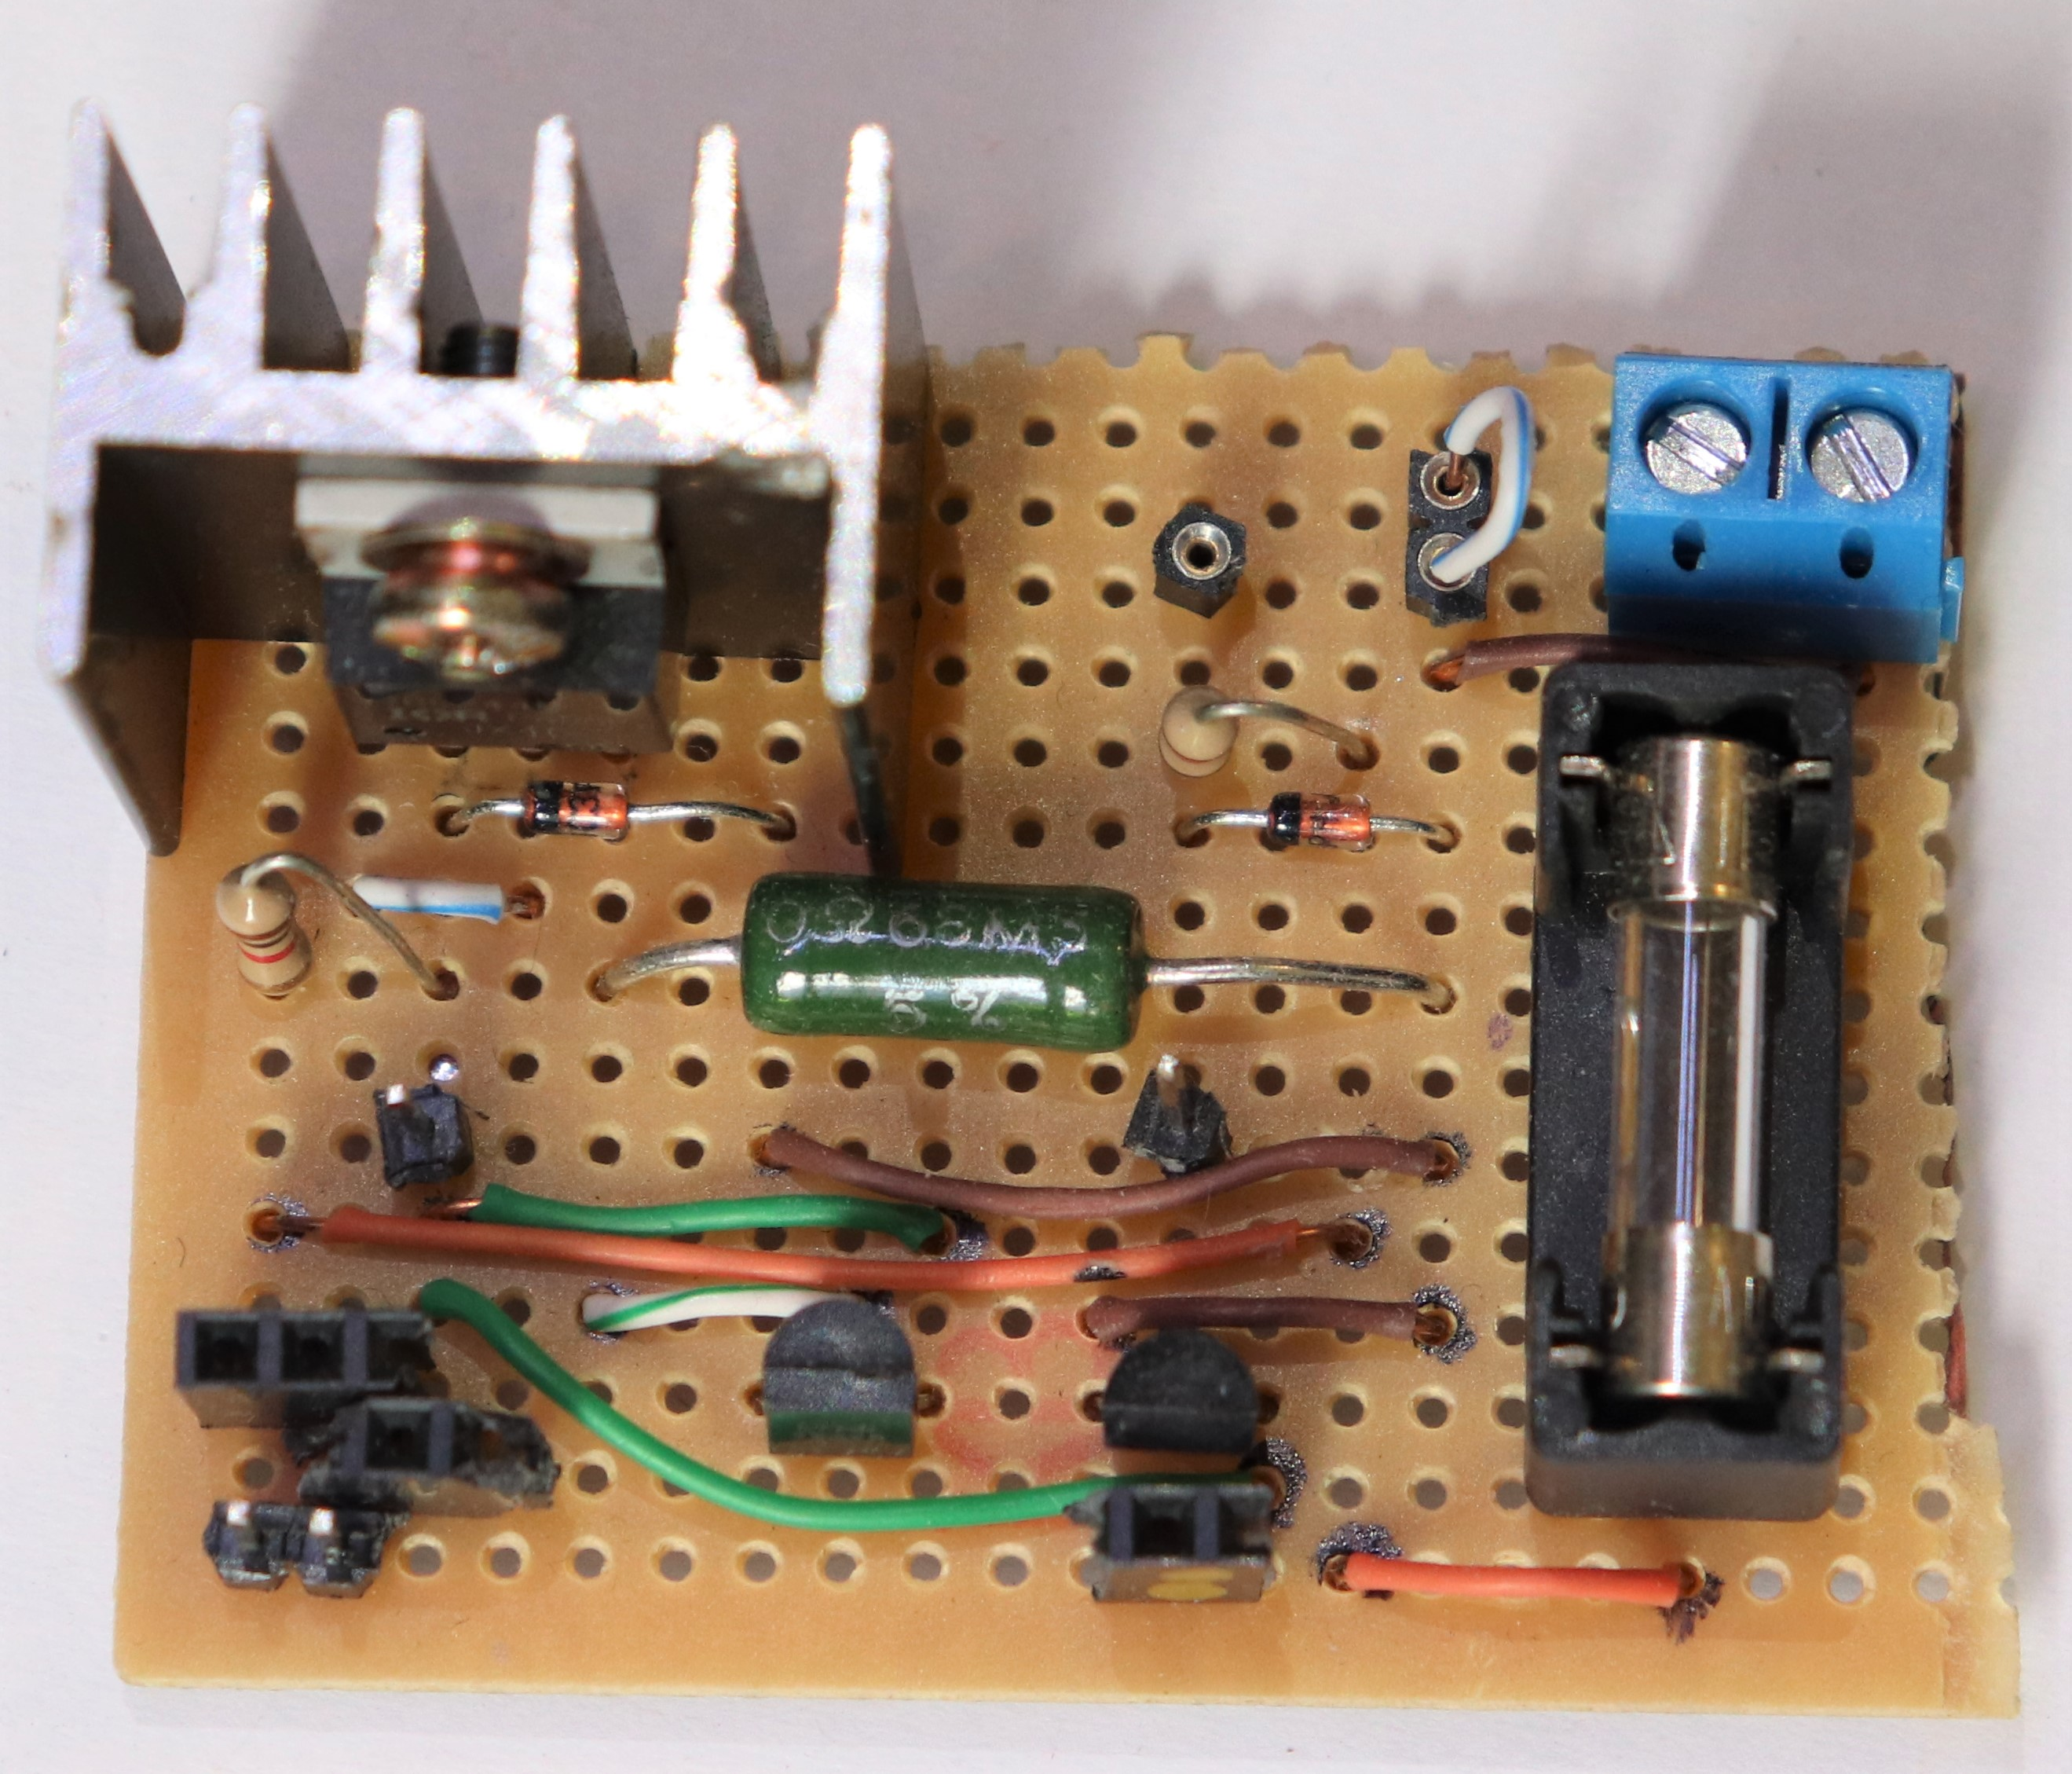
\includegraphics[width=.6\textwidth]{figures/modules/power_led_driver.jpg}
	\caption{Power LED Driver Module}
	\label{fig:module_power_led_driver}
\end{figure}



%%%%%%%%%%%%%%%%%%%%%%%%%%%%%%%%%%%%%%%%%%%%%%%%%%%%%%%%%%%




\subsection{LED Driver}

\subsubsection{Functional Design}
Due to the high power demands of the 3W IR LED, it is more appropriate to perform test and develop the communication protocol using a low power IR led. A separate low power LED driver module was designed for this specific purpose.

The module is designed to be pin-to-pin compatible with the power LED driver module, operating on the same input signal produced by an open-collector driven pin. Pulling the input low causes the LED to illuminate.



\subsubsection{Schematic}
Figure \ref{fig:schematic_low_power_led_driver} shows the schematic for this driver module.

\begin{figure}[H]
	\centering
	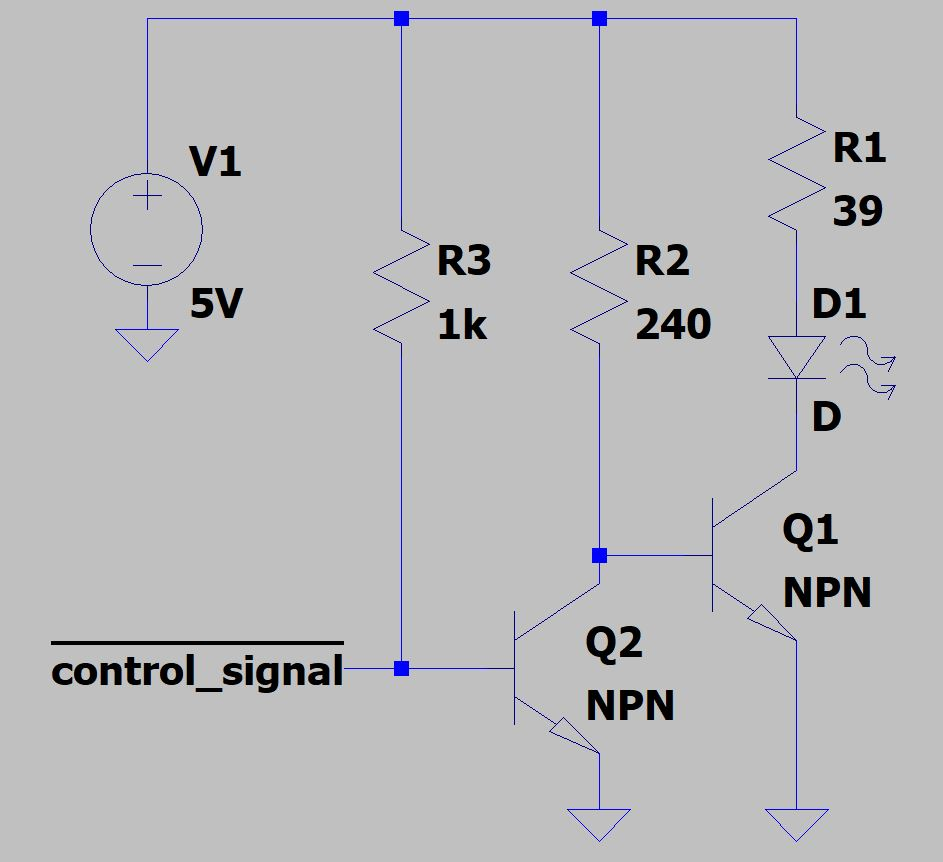
\includegraphics[width=.6\textwidth]{figures/design/low_power_led_driver.JPG}
	\caption{Low-Power LED Driver Module Schematic}
	\label{fig:schematic_low_power_led_driver}
\end{figure}

\subsubsection{Constant Current Control}
%todo: explain how constant current is created



\subsubsection{Module Realization}
The strip-board implementation of the module is shown in figure \ref{fig:module_led_driver} below.

\begin{figure}[H]
	\centering
	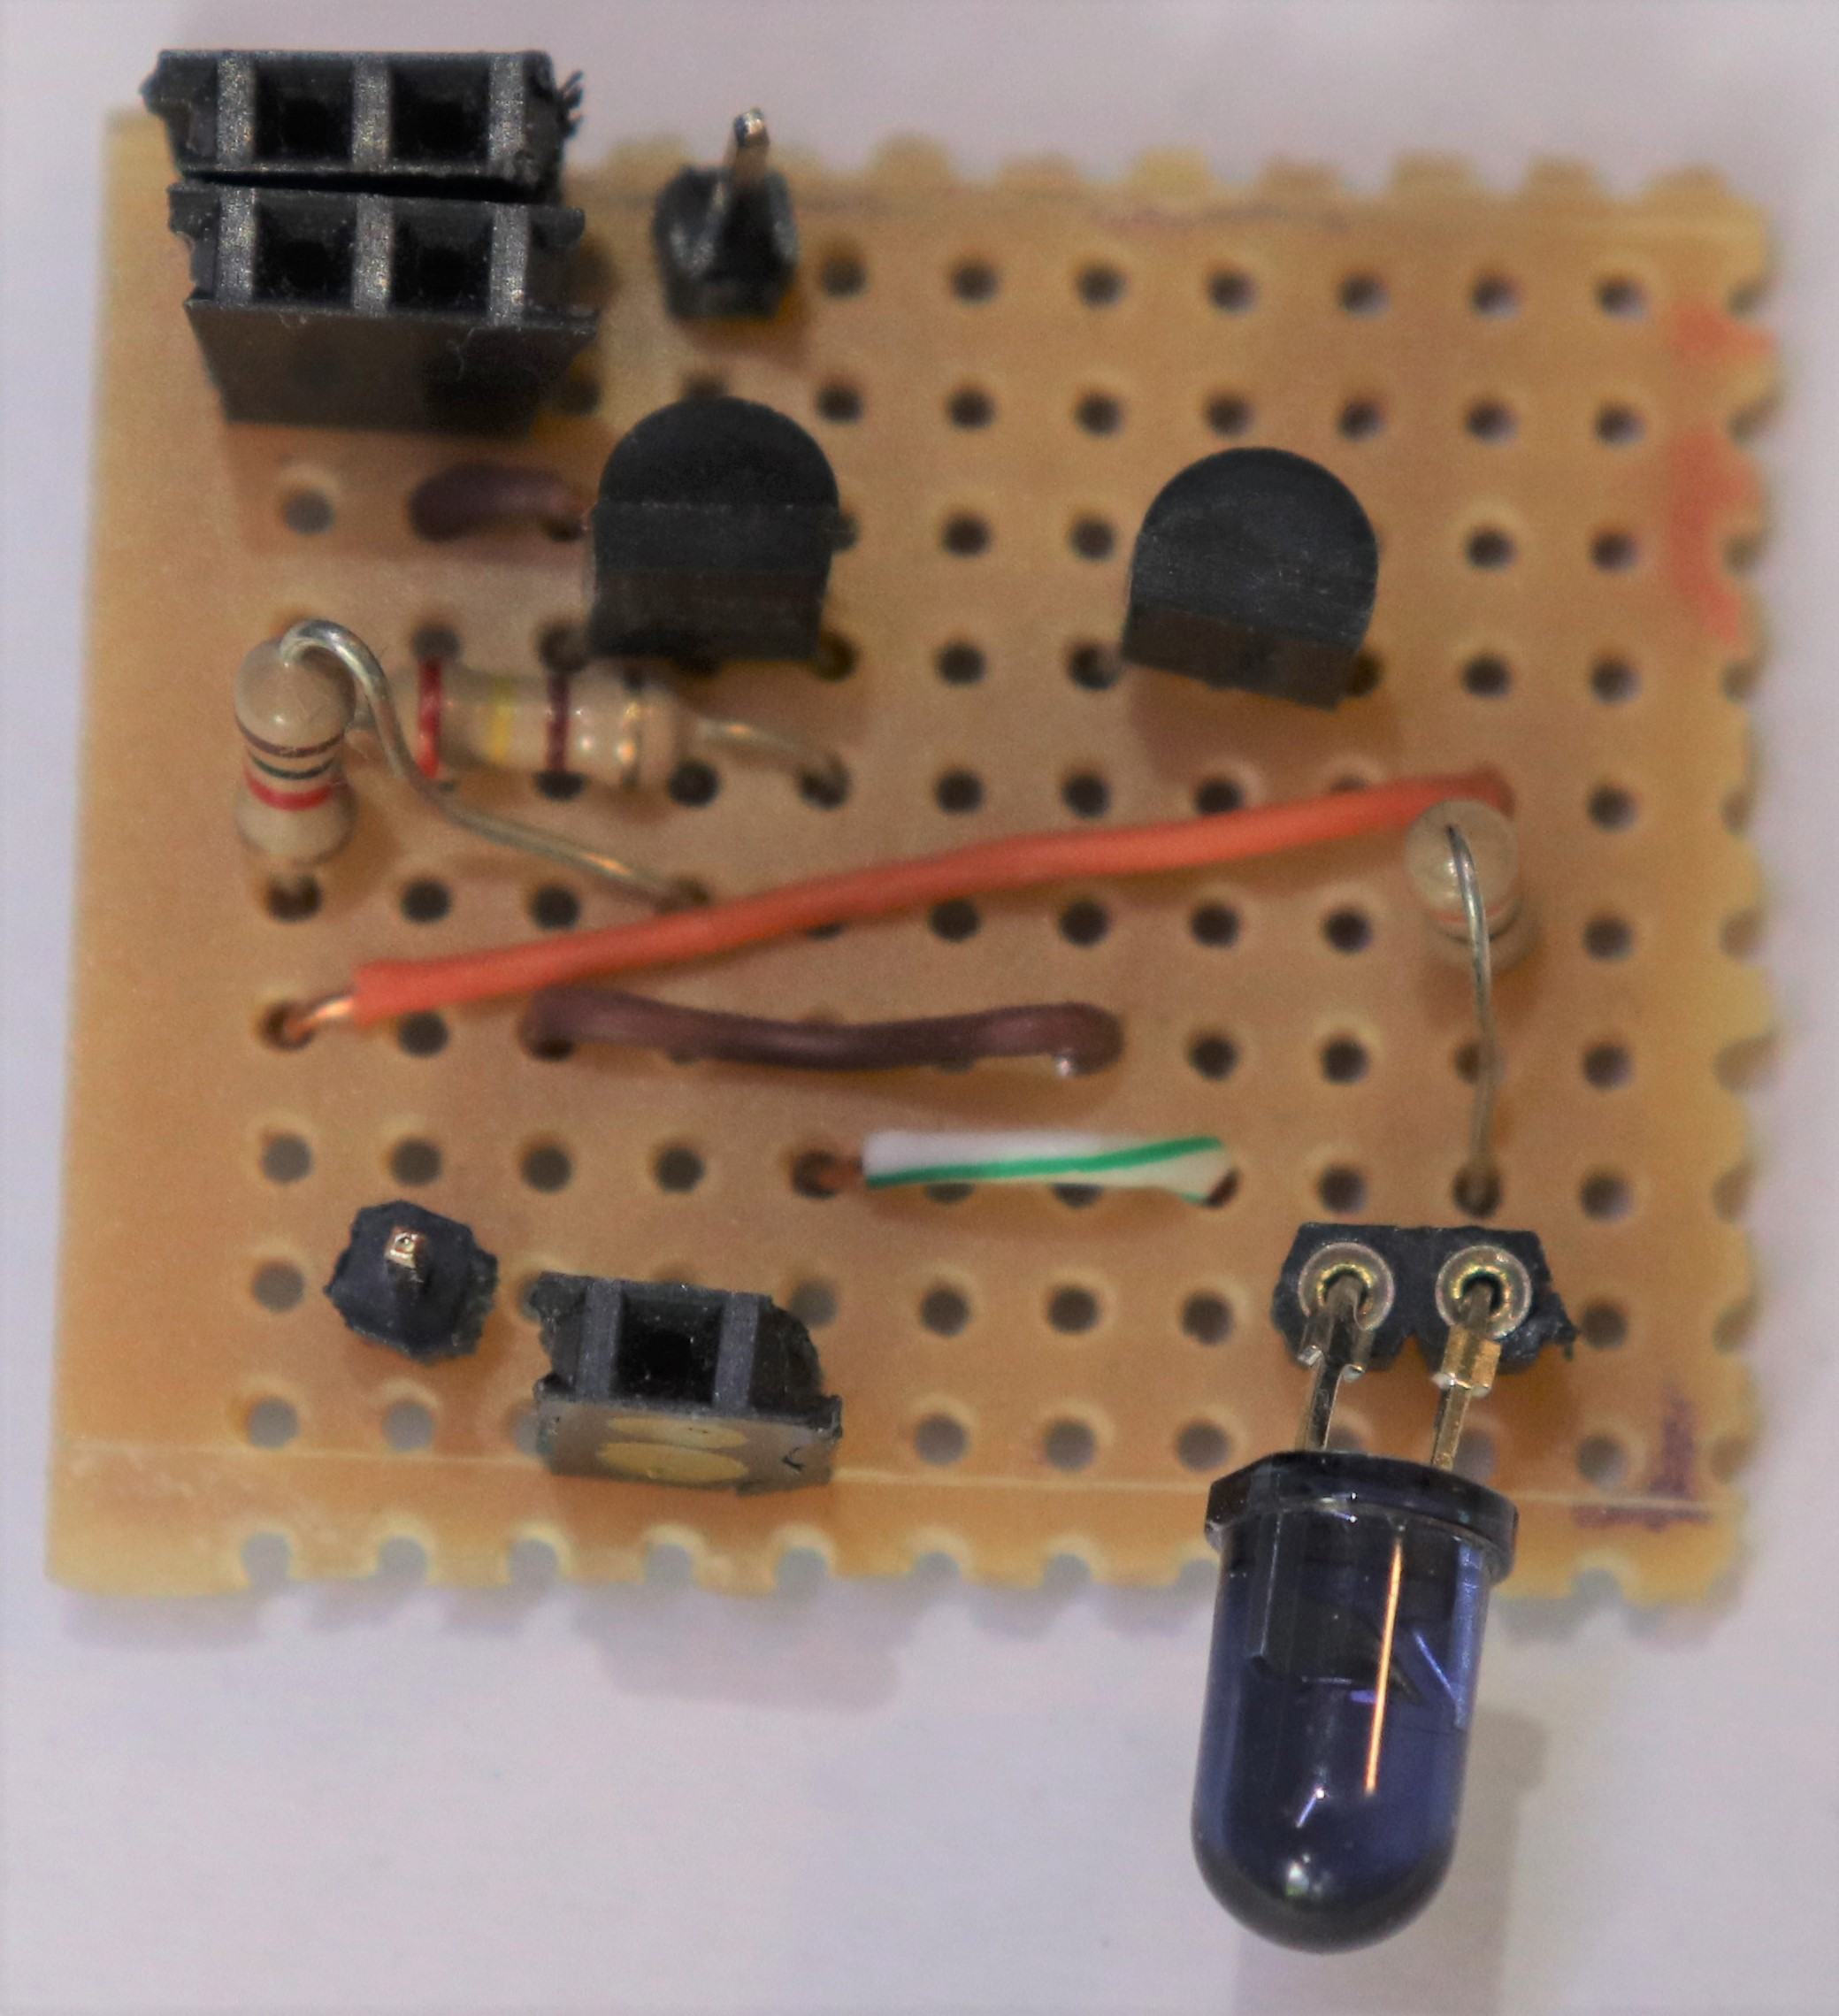
\includegraphics[width=.6\textwidth]{figures/modules/led_driver.jpg}
	\caption{LED Driver Module}
	\label{fig:module_led_driver}
\end{figure}




%%%%%%%%%%%%%%%%%%%%%%%%%%%%%%%%%%%%%%%%%%%%%%%%%%%%%%%%%%%




\subsection{Power LED Focus System}

\subsubsection{Functional Design}
The high power IR LED has a nominally wide beam angle. The function of the LED focus system is to efficiently generate a narrow beam of IR from this light source. This was achieved by using a lens to focus the light into a parallel beam and using a tube to prevent the light not passing through the lens from spilling into the surrounding environment.


\subsubsection{Construction}
Figure \ref{fig:light_focusing_tube} below shows an exploded view of this hardware module. The diagram lists the components used to construct the light focusing tube.

\begin{figure}[H]
	\centering
	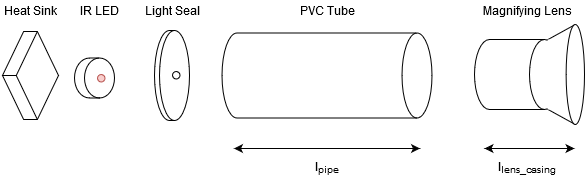
\includegraphics[width=.8\textwidth]{figures/design/beam_tube.png}
	\caption{Exploded View - Light Focusing Tube}
	\label{fig:light_focusing_tube}
\end{figure}

\paragraph{Component Dimensions}
The magnifying lens casing had a length of 30mm, the lens is in-set by 1mm and 3mm of the casing remains external to the tube. The experimental result from section \ref{exp:focal_length} calculated the focal length to be 53mm.

\subsubsection{Light Focusing}

A narrow beam of parallel rays of light may be formed using a point source and ideal lens. Approximating the LED as a point source and the magnifying lens as ideal, a narrow beam may be generated by positioning the light source one focal length away from the lens.

The distance between the light source and lens can be calculated according to equation \ref{eqn:tube_length}.

\begin{equation}
	d_{source-lens} = l_{tube} - l_{lens\_casing} + (l_{lens\_inset\_distance} + l_{lens\_external}) + l_{light\_seal\_thickness}
	\label{eqn:tube_length}
\end{equation}

$d_{source-lens}$ is the distance between the light source and the lens. $l_{tube}$ is the length of the tube. $l_{lens\_casing}$ is the length of the magnifying lens casing as illustrated in figure \ref{fig:light_focusing_tube}, $l_{lens\_inset\_distance}$ is the amount by which the lens is in-set inside the casing and $l_{lens\_external}$ is a measure of the length of casing that remains external to the tube. $l_{light\_seal\_thickness}$ is a measure of the thickness of the hard-board used to form the light seal.

The length $l_{tube}$ was calculated by substituting the experimentally determined focal length into the equation as the length $d_{source-lens}$.

Substituting these values into equation \ref{eqn:tube_length}, the length $l_{tube}$ was calculated

\[l_{tube} = d_{source-lens} + l_{lens\_casing} - (l_{lens\_inset\_distance} + l_{lens\_external}) - l_{light\_seal\_thickness}\]

\[l_{tube} = 53mm + 30mm - (1mm + 3mm) - 3mm = 76mm\]


\subsubsection{Module Realization}
The implementation of the light focus system is shown in figure \ref{fig:module_light_focus} below. Excluded from this image is the IR led and heat-sink.

\begin{figure}[H]
	\centering
	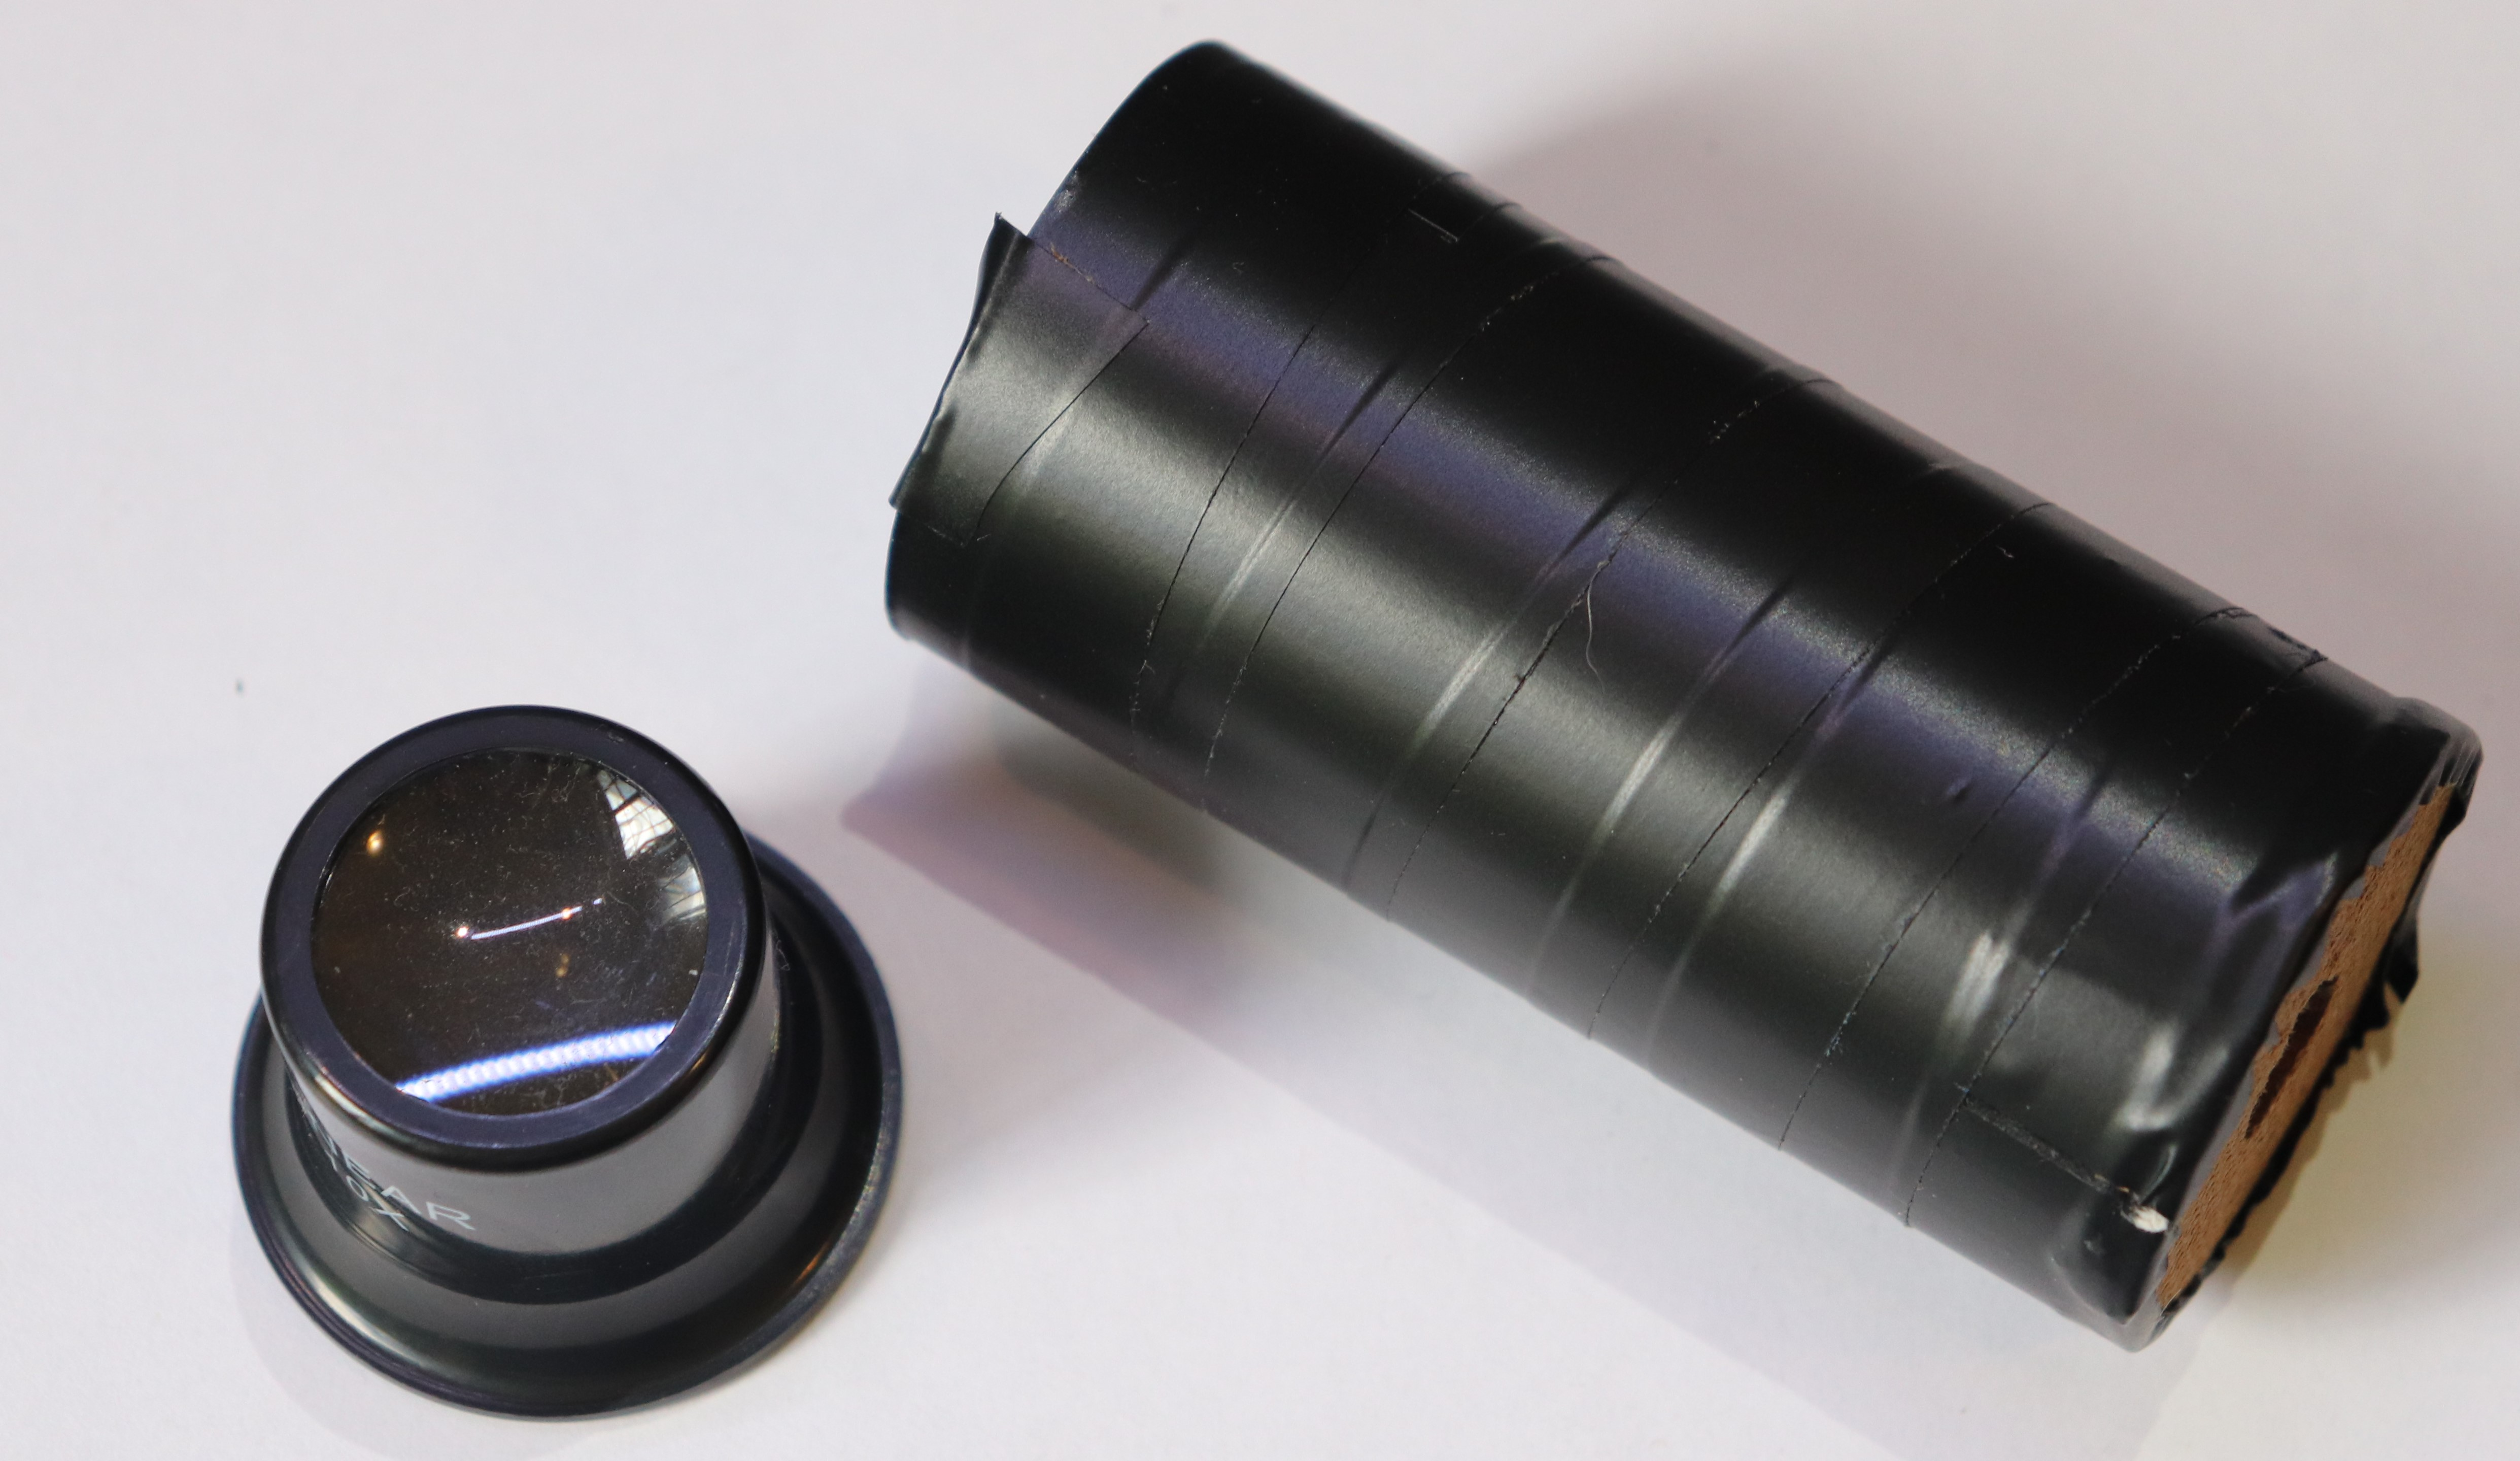
\includegraphics[width=.6\textwidth]{figures/modules/light_focus_tube_lens.jpg}
	\caption{Light Focus System}
	\label{fig:module_light_focus}
\end{figure}



%%%%%%%%%%%%%%%%%%%%%%%%%%%%%%%%%%%%%%%%%%%%%%%%%%%%%%%%%%%




\subsection{Photodiode IR Detector}
%Missing:
% - Schematic and explaination
% - Talk about MCP6022 and important specs

\subsubsection{Functional Design}
The photodiode IR detector module is designed to convert fluctuations in infrared radiation into a voltage signal. The circuit is designed to produce an output voltage proportional to changes in the current flowing through the photodiode.


\subsubsection{Schematic}
Figure \ref{fig:schematic_photodiode_transimpedance} below shows the schematic for the module. The circuit is inspired by S. Schrires 'Infrared Radio Link' circuit which is found in the EEE3071 course notes \cite{Schrire2007}.


\begin{figure}[H]
	\centering
	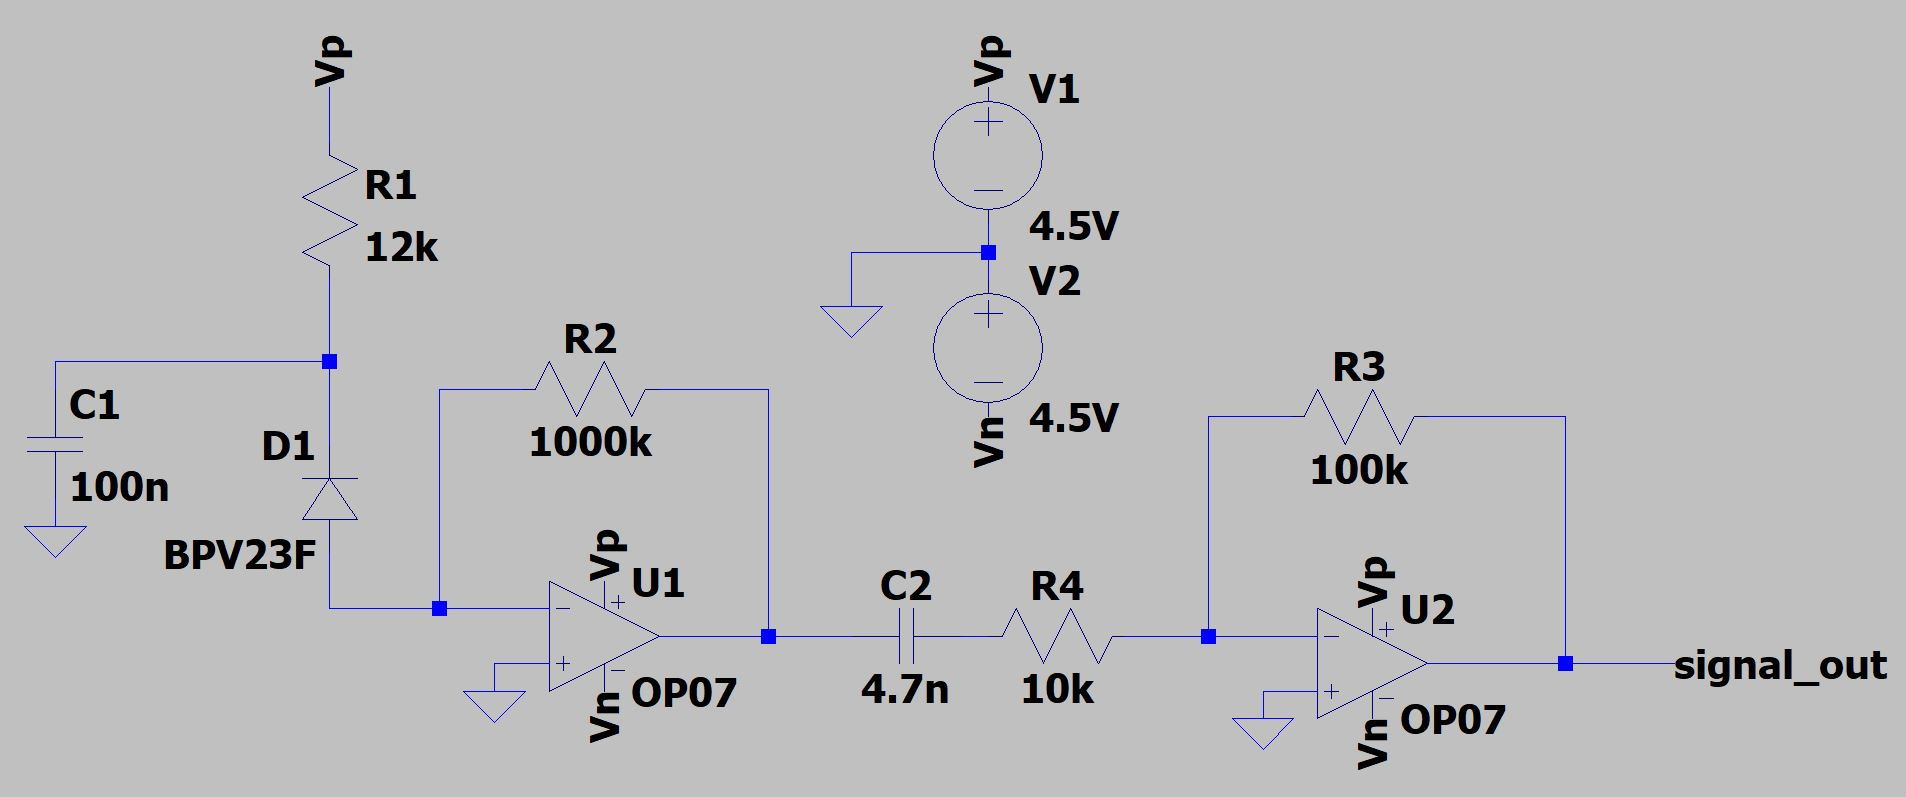
\includegraphics[width=.8\textwidth]{figures/design/photodiode_transimpedance.JPG}
	\caption{Photodiode IR Detector Module Schematic}
	\label{fig:schematic_photodiode_transimpedance}
\end{figure}

\subsubsection{Trans-impedance Amplifier}
%todo: this needs to be completed


\subsubsection{Module Realization}
The strip-board implementation of the module is shown in figure \ref{fig:module_photodiode_receiver} below.

\begin{figure}[H]
	\centering
	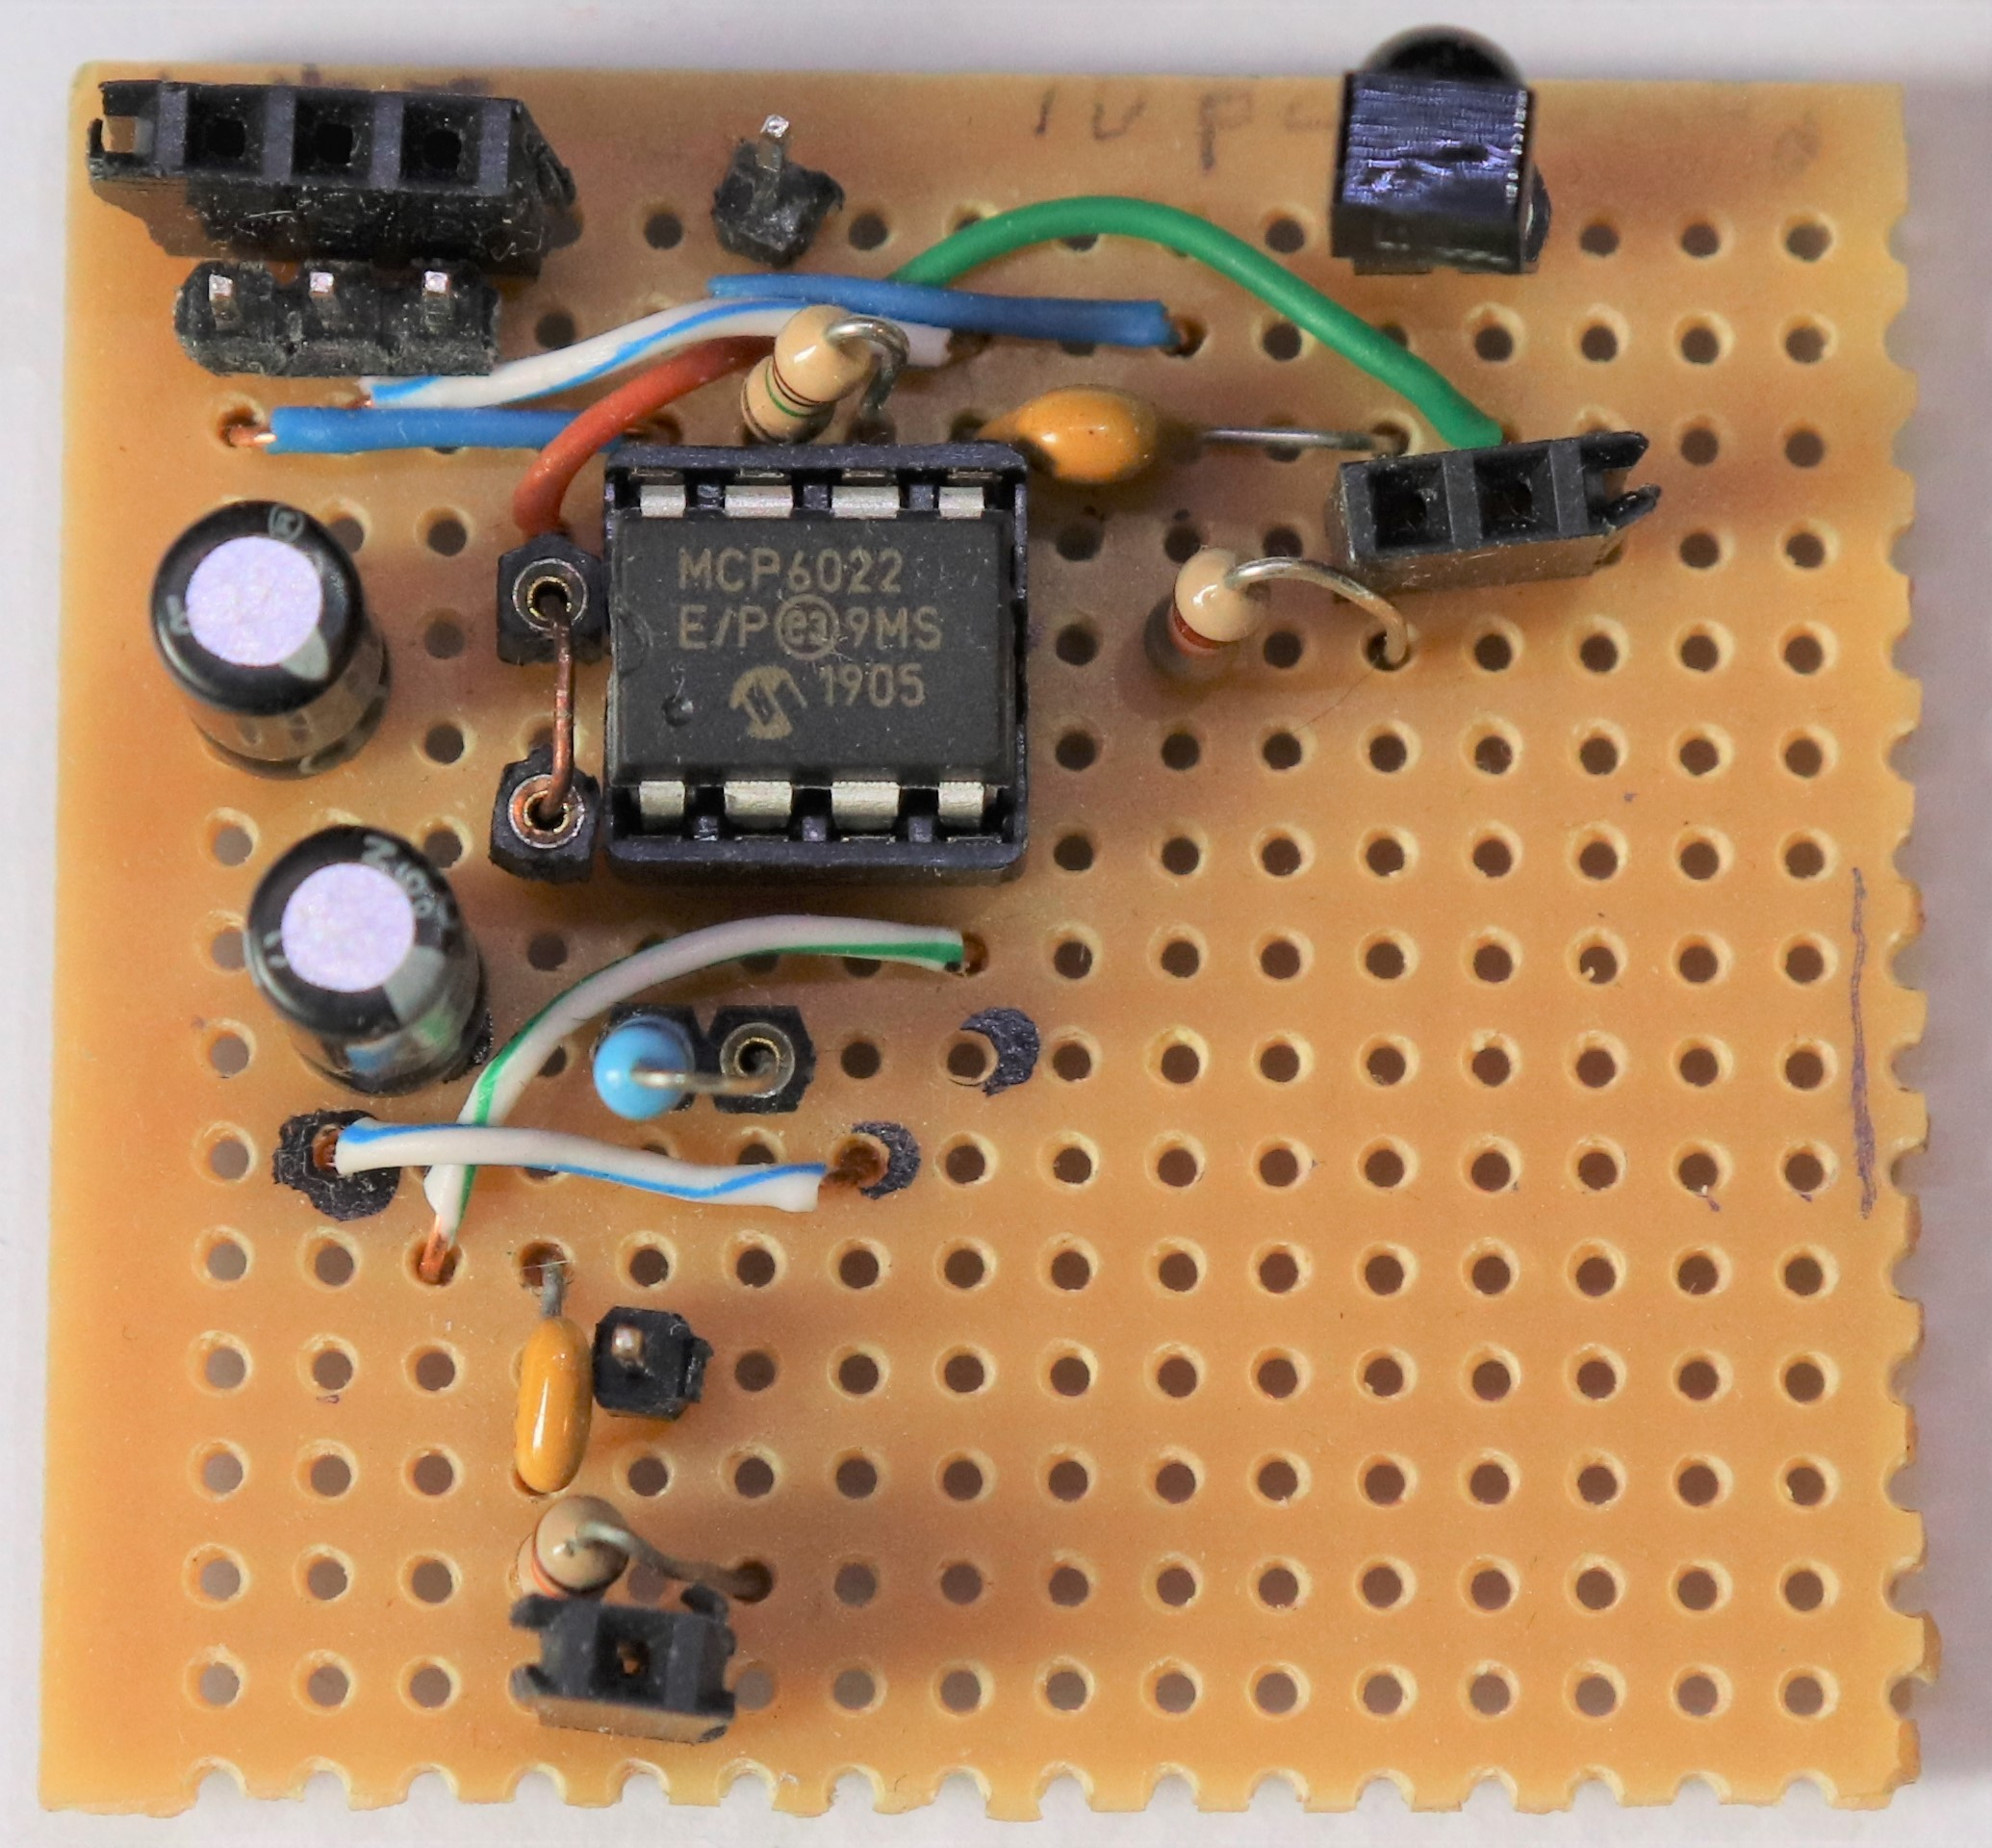
\includegraphics[width=.6\textwidth]{figures/modules/photodiode_receiver.jpg}
	\caption{Photodiode IR Receiver Module}
	\label{fig:module_photodiode_receiver}
\end{figure}


%%%%%%%%%%%%%%%%%%%%%%%%%%%%%%%%%%%%%%%%%%%%%%%%%%%%%%%%%%%



\subsection{Phototransistor IR Detector}
%todo:
% - Schematic and explaination

\subsubsection{Functional Design}
The phototransistor IR detector module, like the photodiode IR detector module, is designed to convert fluctuation in infrared radiation into a voltage signal. The circuit is designed to produce an output voltage proportional to changes in the current flowing through the phototransistor.

\subsubsection{Schematic}
Figure \ref{fig:schematic_phototransistor_detector} below shows the schematic for the module.


\begin{figure}[H]
	\centering
	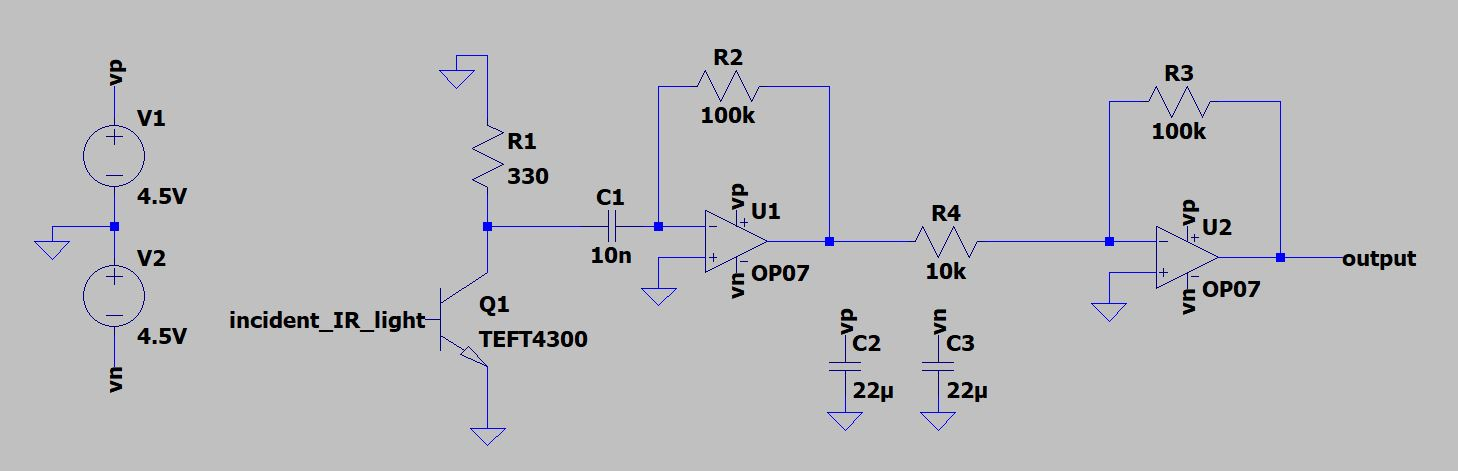
\includegraphics[width=.9\textwidth]{figures/design/phototransistor_detector.JPG}
	\caption{Phototransistor IR Detector Module Schematic}
	\label{fig:schematic_phototransistor_detector}
\end{figure}

\subsubsection{Trans-impedance Amplifier}
%todo: this needs to be completed


\subsubsection{Module Realization}
The strip-board implementation of the module is shown in figure \ref{fig:module_photodiode_receiver} below.

\begin{figure}[H]
	\centering
	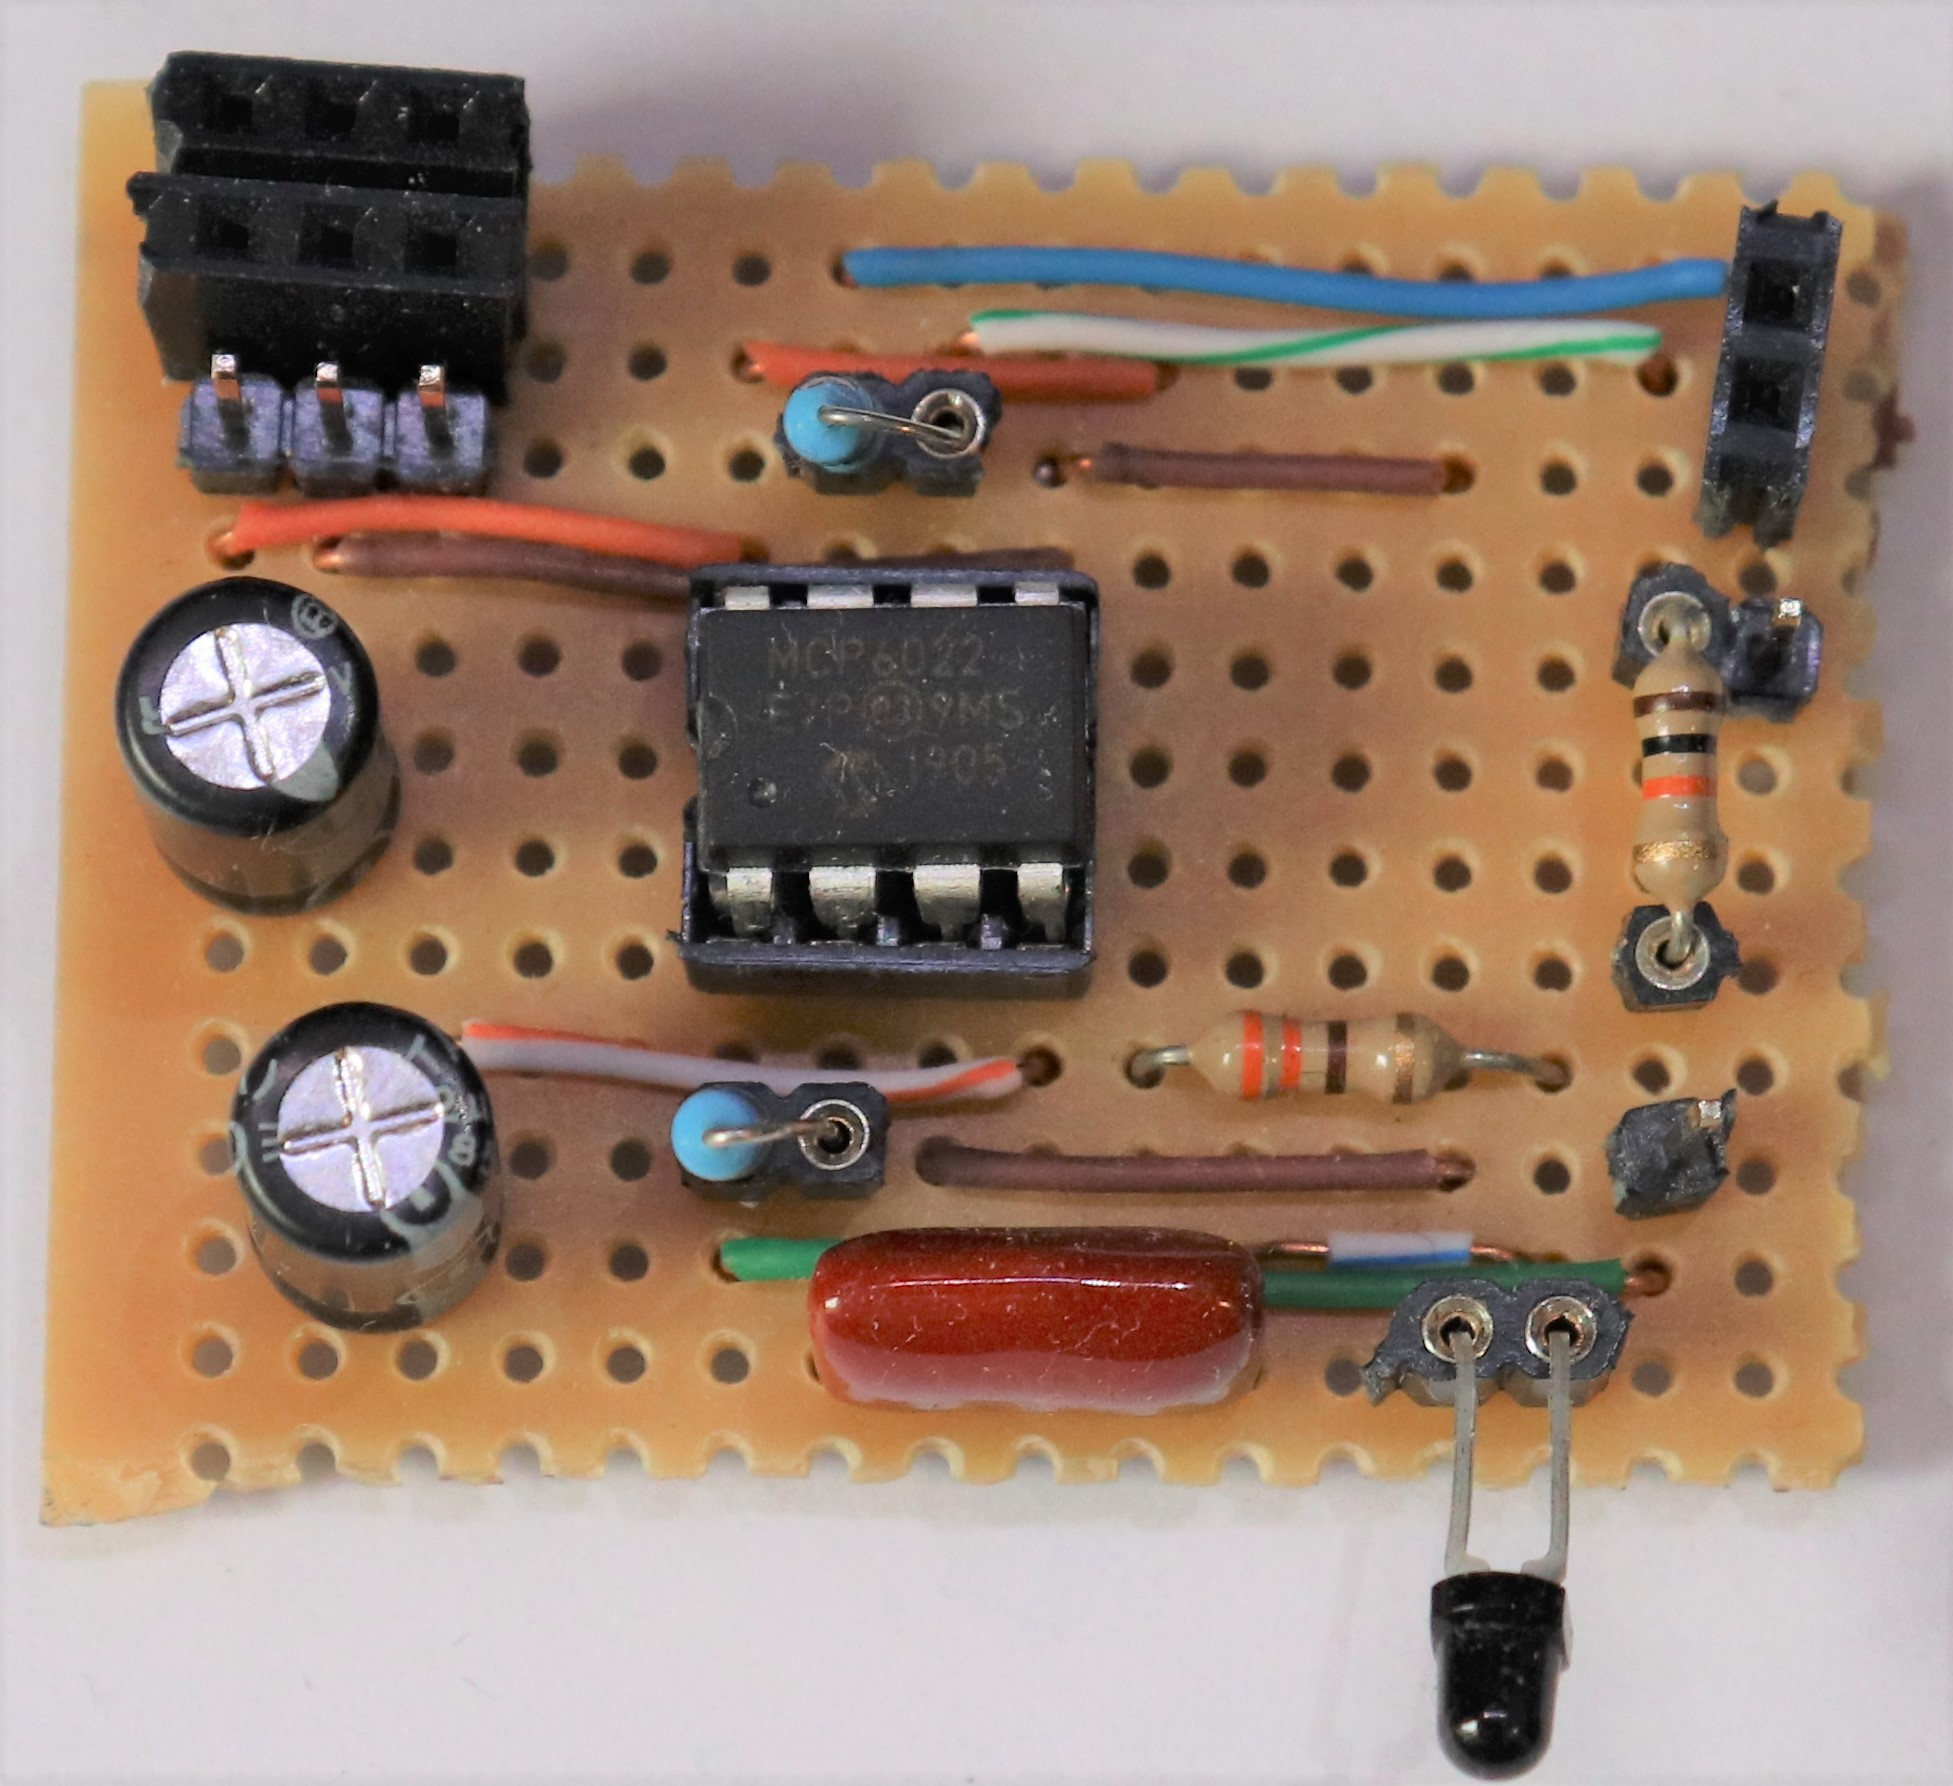
\includegraphics[width=.6\textwidth]{figures/modules/phototransistor_receiver.jpg}
	\caption{Phototransistor IR Detector Module}
	\label{fig:module_phototransistor_detector}
\end{figure}




%%%%%%%%%%%%%%%%%%%%%%%%%%%%%%%%%%%%%%%%%%%%%%%%%%%%%%%%%%%




\subsection{IR Receiver}
%Missing:
% - Schematic and explaination

The IR receiver is an 'all in one package' detector IC designed to detect the presences of a carrier signal in the IR light incident on the detector.

\begin{figure}[H]
	\centering
	\begin{minipage}{.5\textwidth}
		\centering
		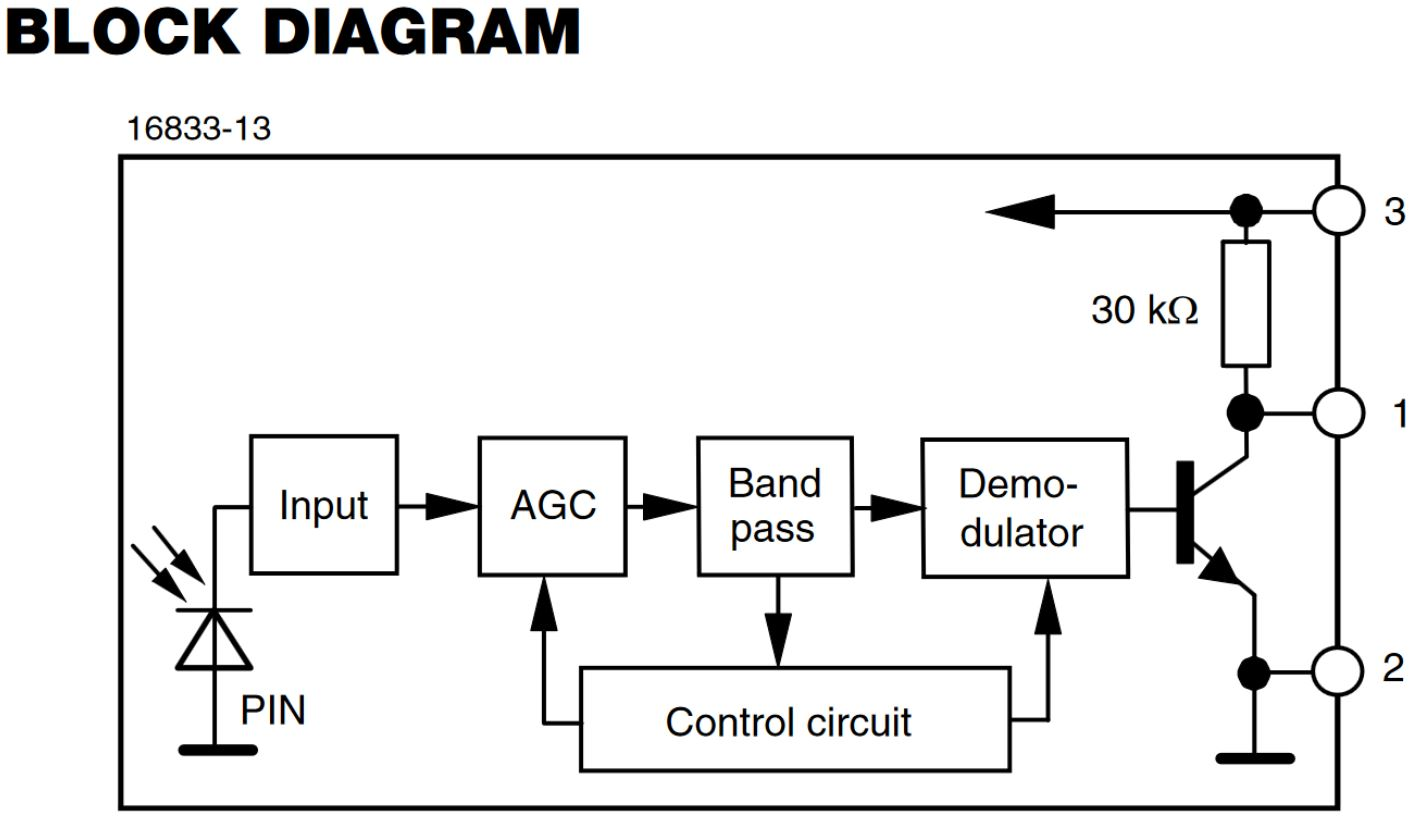
\includegraphics[width=.8\linewidth]{figures/design/TSOP382_block_diagram}
		\captionof{figure}{TSOP382 Functional Diagram}
		\label{fig:tsop382_block_diagram}
	\end{minipage}%
	\begin{minipage}{.5\textwidth}
		\centering
		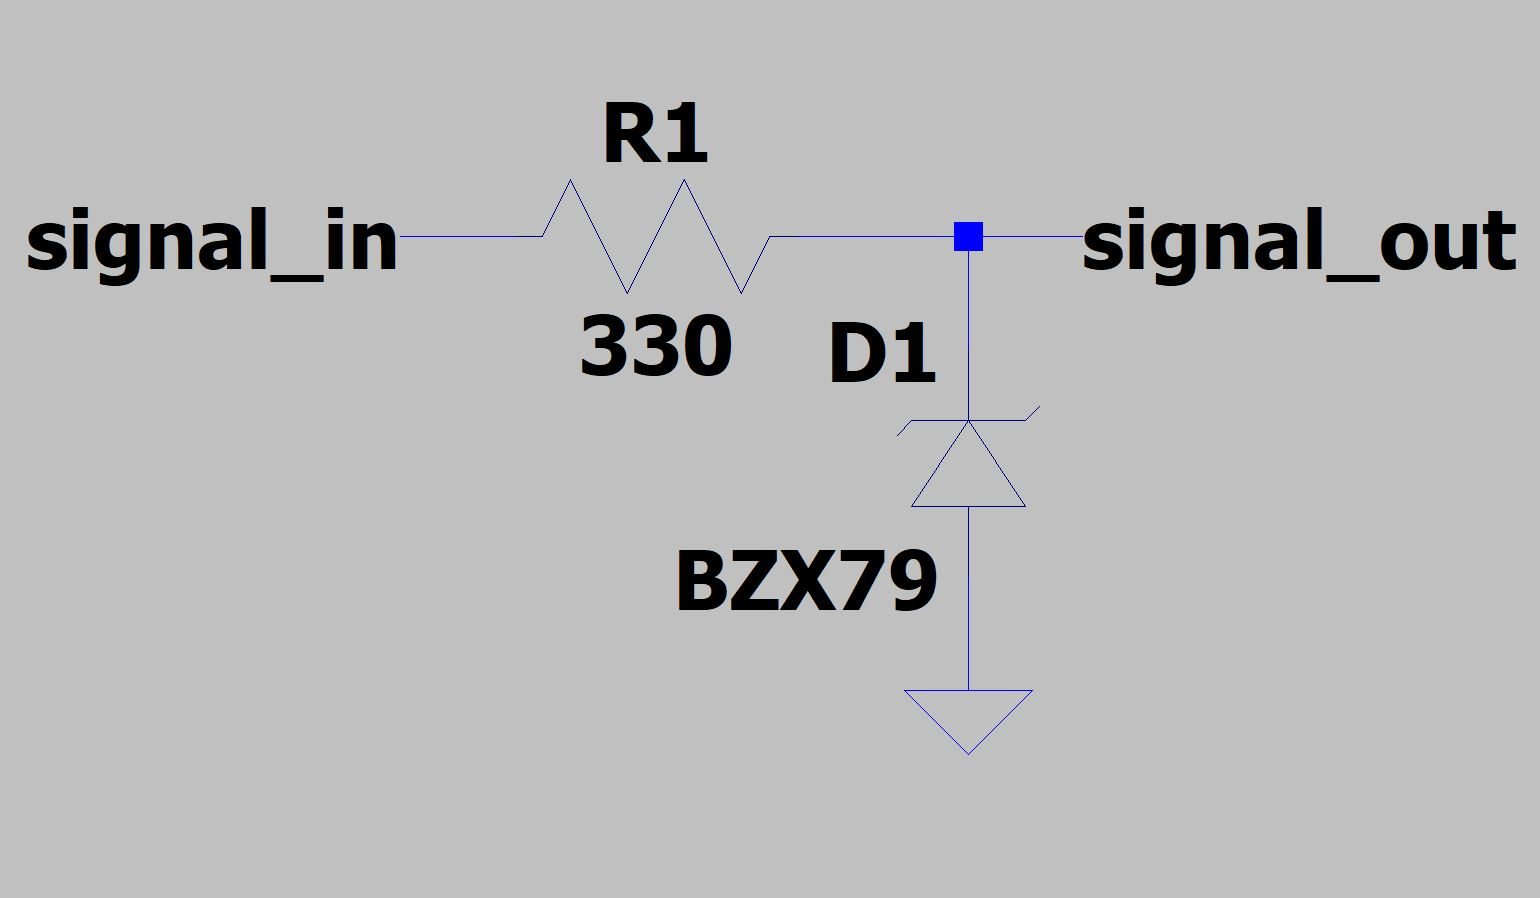
\includegraphics[width=.8\linewidth]{figures/design/over_voltage_protection}
		\captionof{figure}{Voltage Clamp}
		\label{fig:schematic_voltage_clamp}
	\end{minipage}
\end{figure}

The IR receiver used in this investigation is the TSOP382 from Vishay. The \href{https://www.vishay.com/docs/82491/tsop382.pdf}{datasheet} contains a block diagram (shown in figure \ref{fig:tsop382_block_diagram}) which gives a functional overview of the IC.

Figure \ref{fig:schematic_voltage_clamp} shows the circuity used to clamp the output of the IR receiver at 3V. This is to protect the GPIO from an over-voltage. The TSOP382 may be powered off 3.3V which would remove the voltage clamp requirement, however it has been included to ensure the module can be powered with a range of supply voltages and still be logically compatible with the STM32.

\begin{figure}[H]
	\centering
	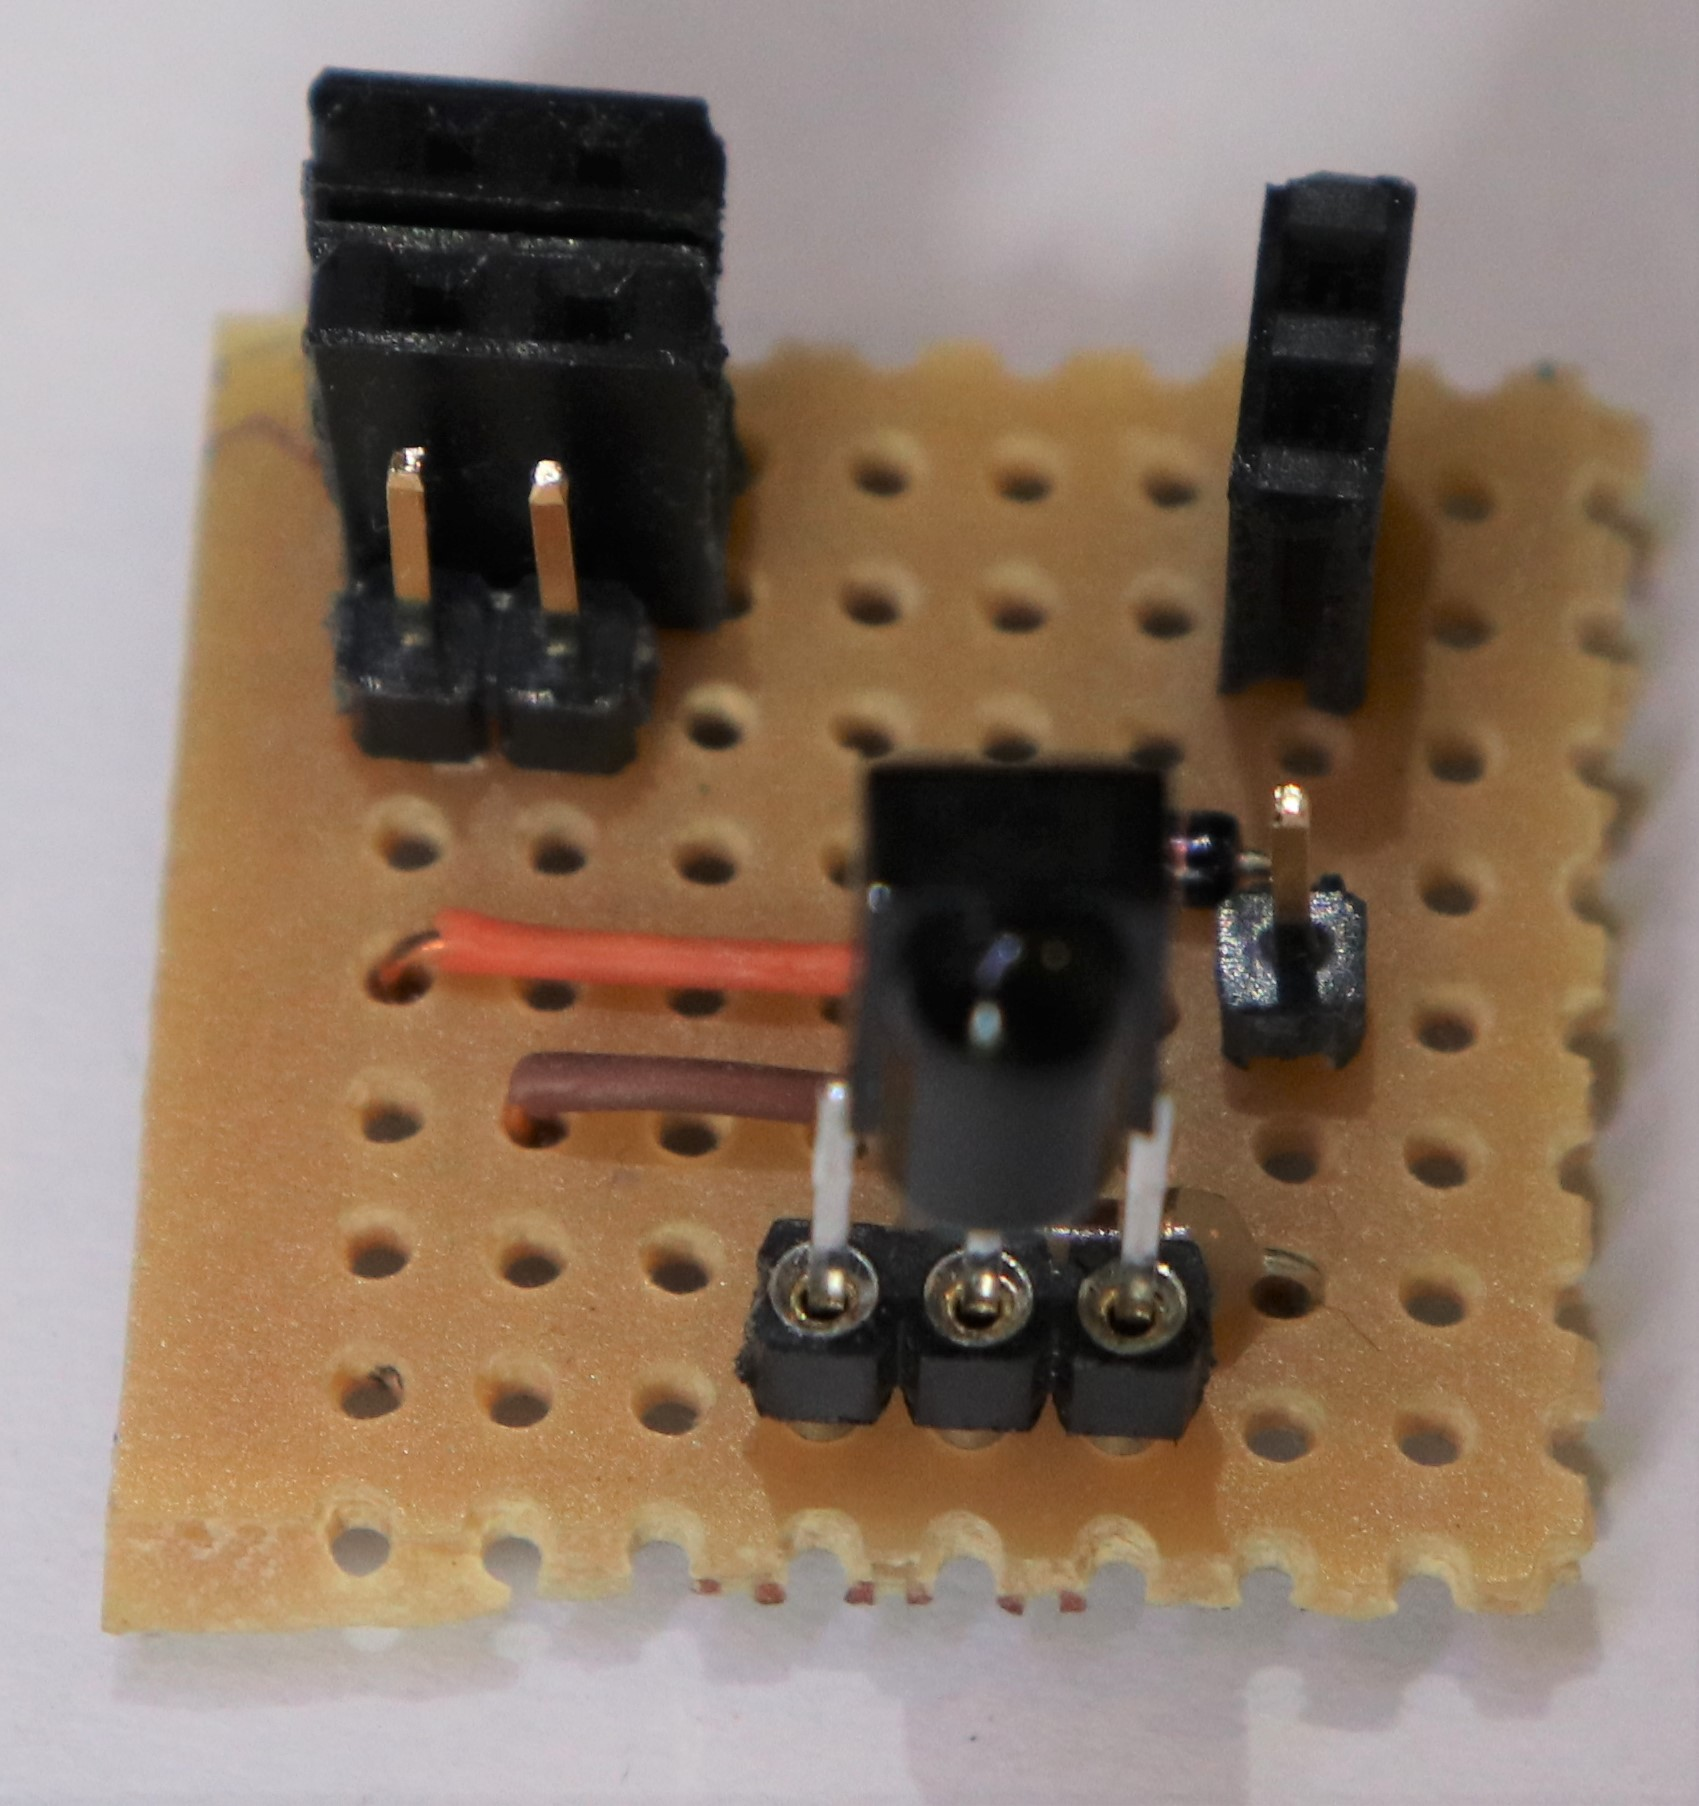
\includegraphics[width=.6\textwidth]{figures/modules/ir_receiver.jpg}
	\caption{IR Receiver Module}
	\label{fig:module_ir_receiver}
\end{figure}



%%%%%%%%%%%%%%%%%%%%%%%%%%%%%%%%%%%%%%%%%%%%%%%%%%%%%%%%%%%



\subsection{Signal Conditioning Module}
%Missing:
% - Choosing freq cut off and what is expected gain

The signal conditioning module can be broken into two stages. The first stage of the module performs filtering, this is prevent aliasing during the digital signal processing, which is caused by frequencies greater than half the sampling frequency being present in the sampled waveform. The second stage performs precision rectification, which is necessary to ensure a negative voltage is not placed on the input pin of the tone detector which has a tolerance range from 0V to 3.3V.

\begin{figure}[H]
	\centering
	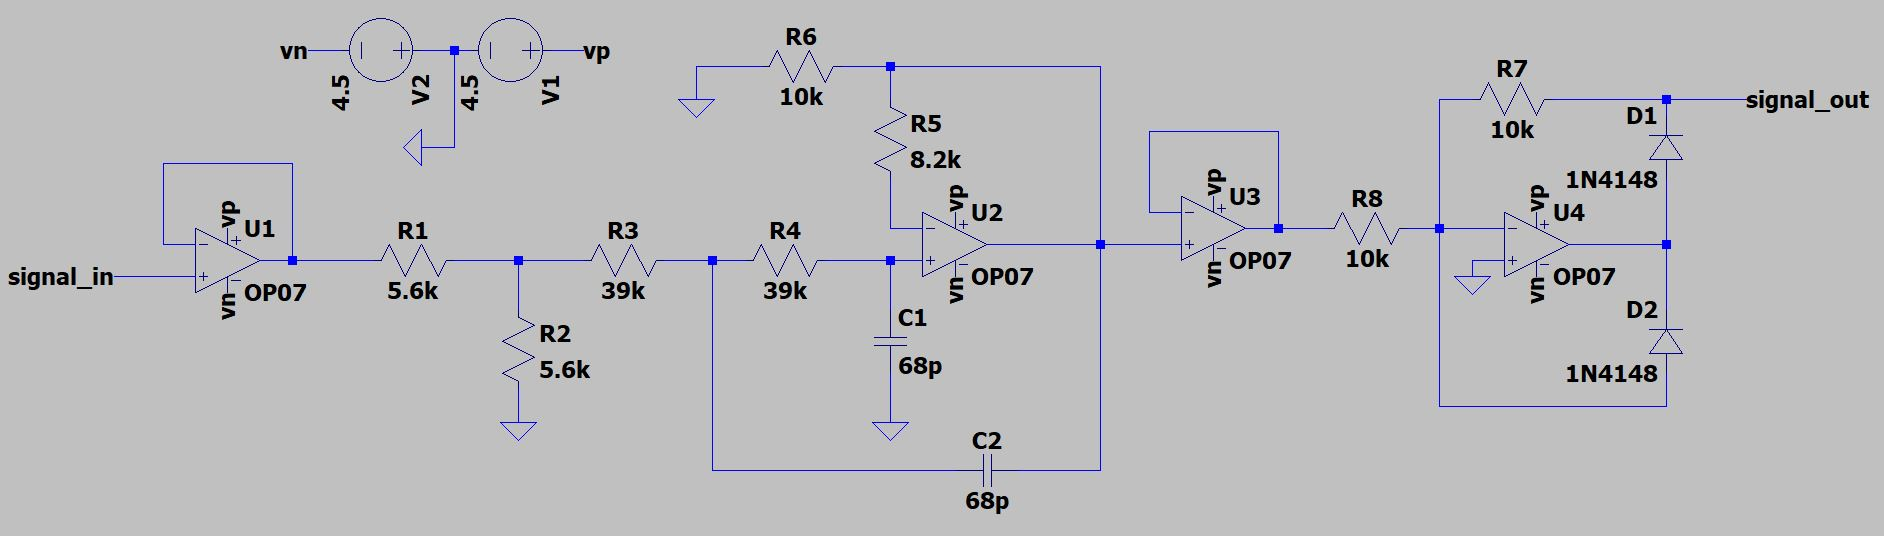
\includegraphics[width=\textwidth]{figures/design/filter_and_rectify}
	\caption{Signal Conditioning Module Schematic}
	\label{fig:schematic_filter_and_rectify}
\end{figure}

In most cases the incoming signal is a square wave which has formed due to the amplification stage of the detector module saturating at $\pm 4.5V$. To ensure the output signal is within the tolerance of the ADC, a voltage divider formed by R1 and R2 filter is place prior to the filter.

The filter circuit used is a second order voltage controlled voltage source (VCVS) active low pass filter in a Chebyshev configuration\footnote{0.5dB passband ripple}. The Chebyshev configuration was chosen because a sharp roll of is desired and because passband ripple will not affect the ability of the Goertzel filter to detect the target frequency. The component values where chosen in accordance to the filter design table found on page 274 of the book \textit{The art of electronics - 2nd Edition}\cite{Horowitz1995}.

The precision rectifier is also a circuit design taken from the book and can be found on page 188, it is an improved version of the basic precision rectifier because it reduces the output swing of the op-amp during operation\cite{Horowitz1995}.

\begin{figure}[H]
	\centering
	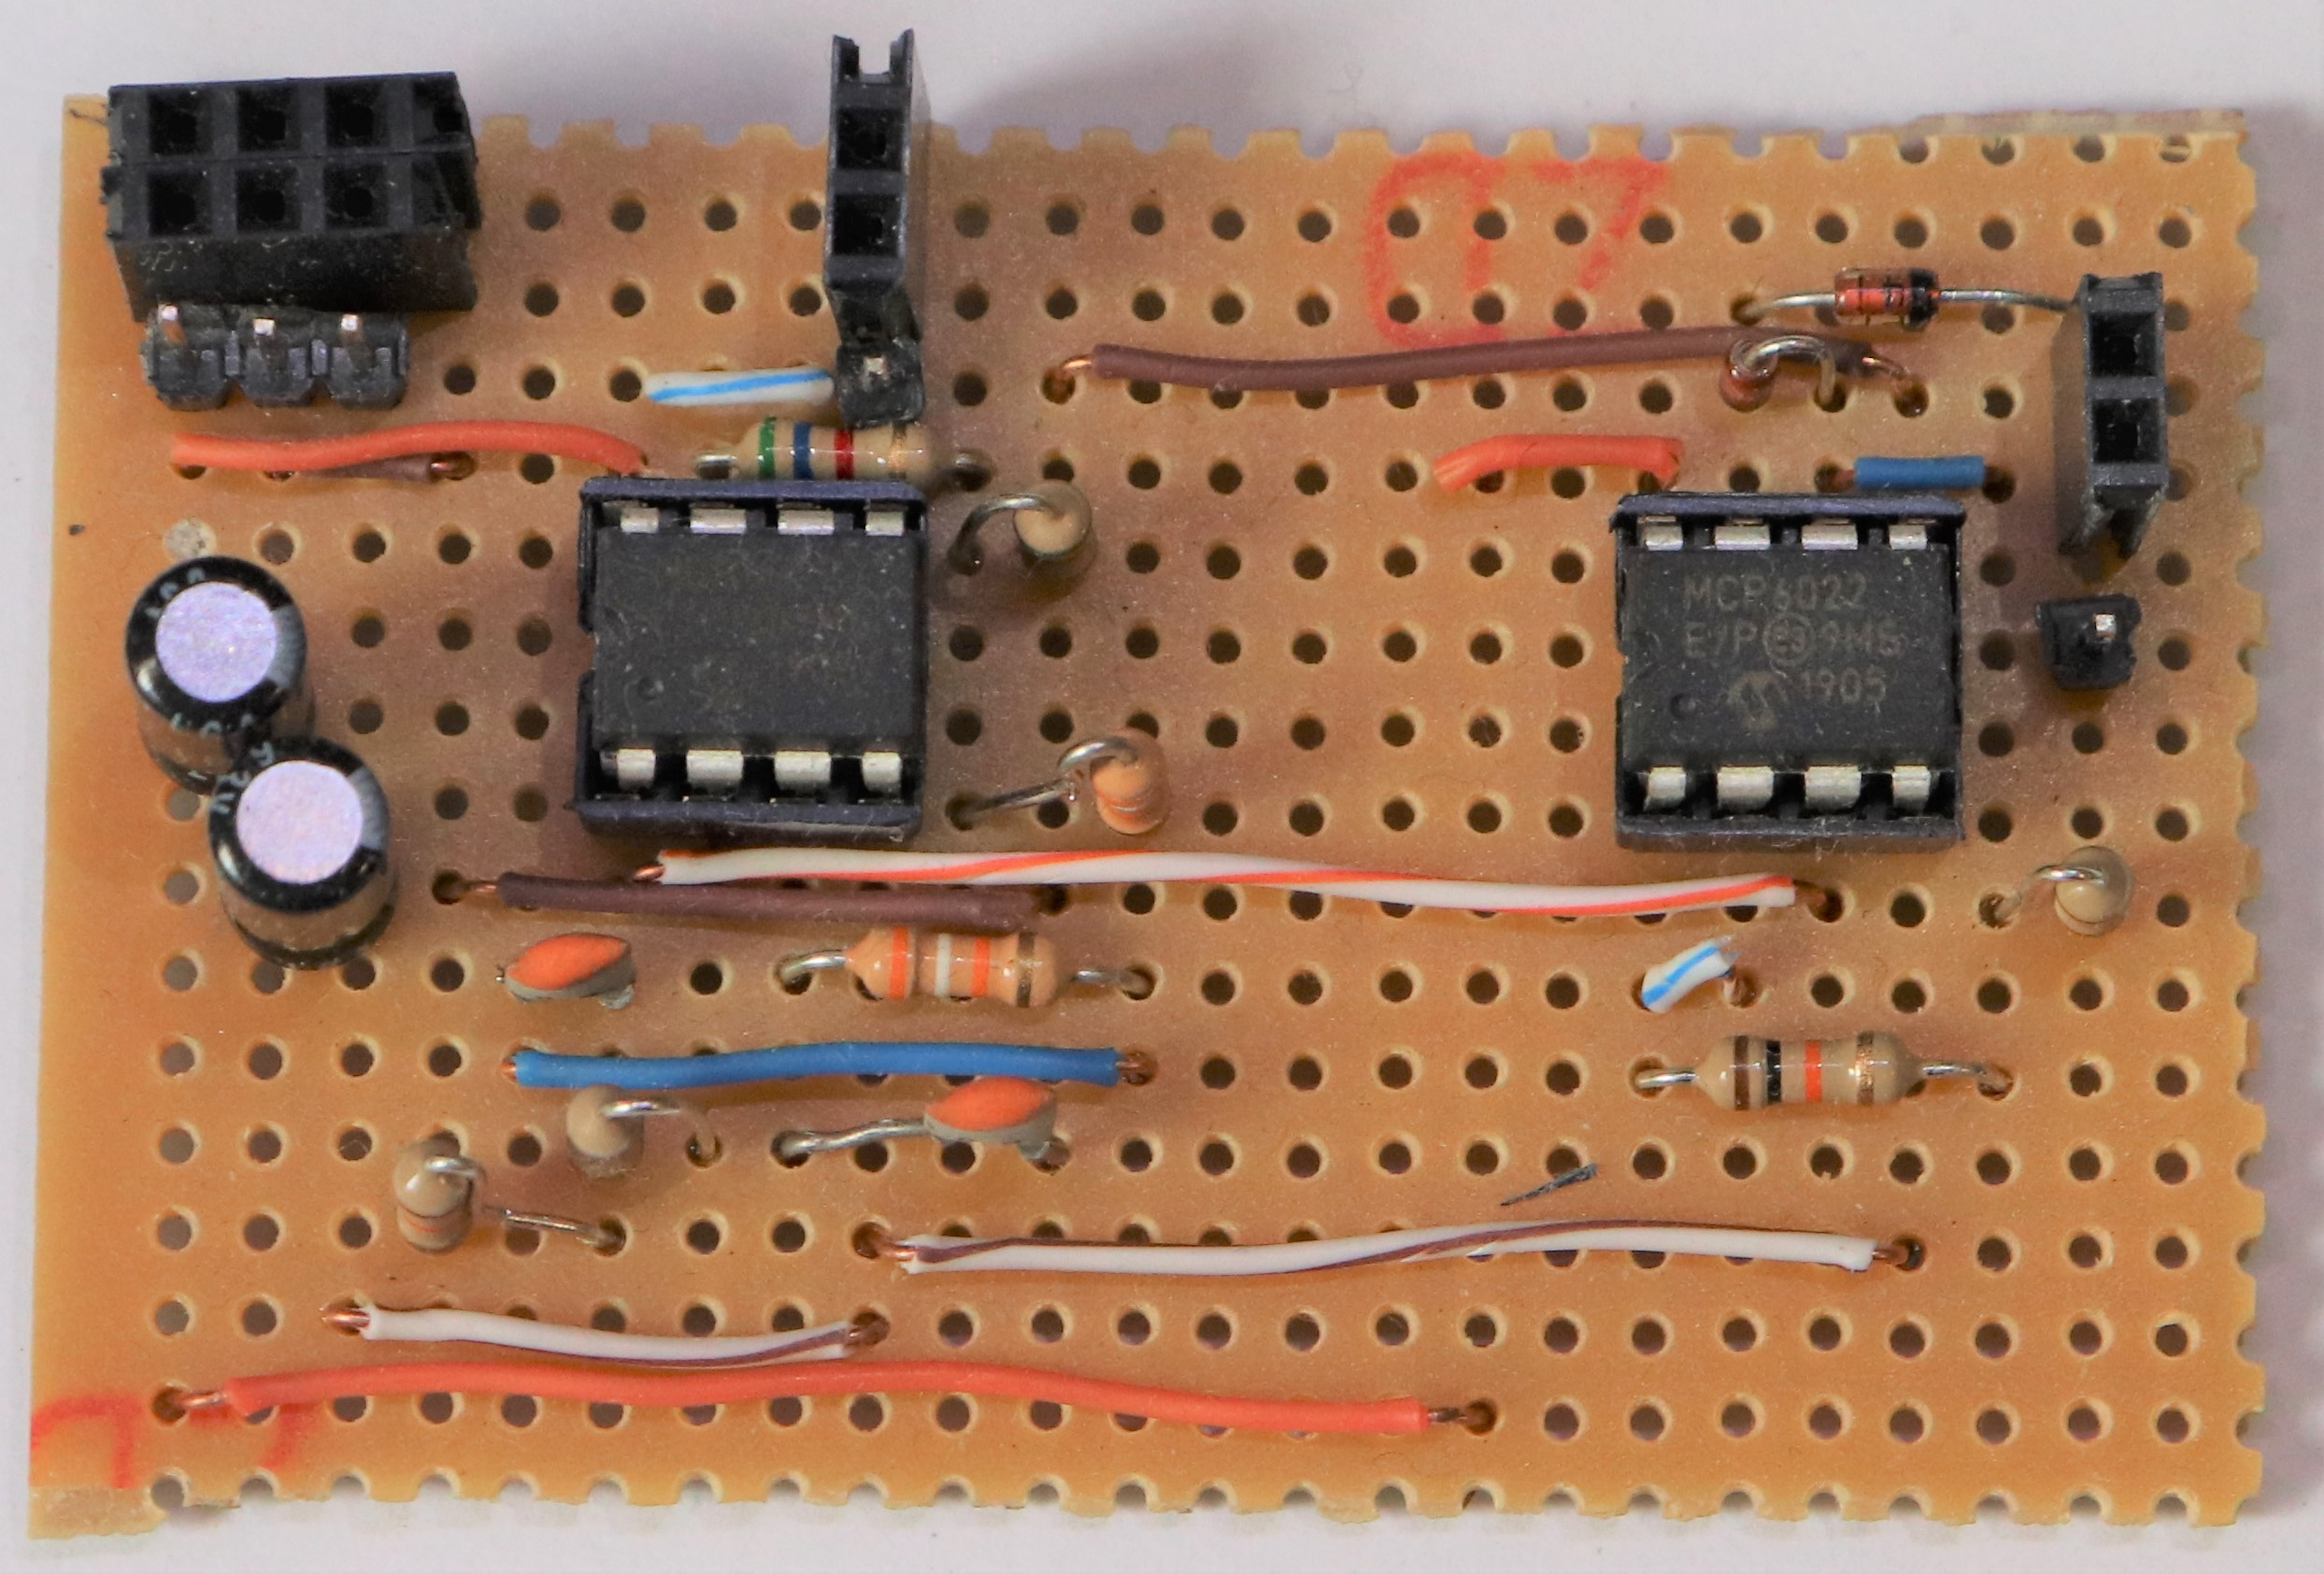
\includegraphics[width=.6\textwidth]{figures/modules/filtering_conditioning.jpg}
	\caption{Signal Conditioning Module}
	\label{fig:module_filtering_conditioning}
\end{figure}




%%%%%%%%%%%%%%%%%%%%%%%%%%%%%%%%%%%%%%%%%%%%%%%%%%%%%%%%%%%



\subsubsection{Filter Design}
%todo: desired freq cutoff and calculations


The desired cut-off frequency is \(f_{c} = 48kHz\), this defines the end of the passband\footnote{Unlike in the case of a Bessel filter, this is not necessarily the -3dB point}.

With reference to the schematic (figure \ref{fig:module_filtering_conditioning}), resistors and capacitors hold the following relations ships: \(R_3 = R_4 = R\) and \(C_1 = C_2 = C\).

According to the lookup table, to achieve a Chebyshev response, the following values should be used as the normalization factor and gain: \(f_n = 1.231\), \(K = 1.842\).

The gain is set by choosing $R_5$ and $R_6$ such that \(R_5 = (K - 1) \times R_6\) holds. The values of $R$ and $C$ are determined by the following equation


\[RC = \frac{1}{2\pi f_n f_c}\]

Substituting into the above equation we find $RC = 2.6935\times 10^{-6}$. It is recommended that the resistance value is between $10k$ and $100k$, the value of $39k\Omega$ was selected. The corresponding capacitance value is calculated to be $69pF$, and the E12 series capacitance value of $68pF$ was used.




%%%%%%%%%%%%%%%%%%%%%%%%%%%%%%%%%%%%%%%%%%%%%%%%%%%%%%%%%%%




\subsection{Tone Decoder Module}
%Missing:
% - Is a schematic worth the bother?

The tone decoder module's hardware consists of an STM32F051C6 breakout PCB which is mounted on a strip-board along with supporting circuity (external crystal and voltage regulation). In addition to the supporting circuitry, an over-voltage protection clamp (see figure \ref{fig:schematic_voltage_clamp}) was placed on pin 17 which is connected internally to PA7 which is configured as an analog input. Three signal LED's where wired to pins 18, 19 and 20 to act as status indicators.

The DSP algorithm is discussed in subsection \ref{tone_decoder_software} from the following section on software modules.


\begin{figure}[H]
	\centering
	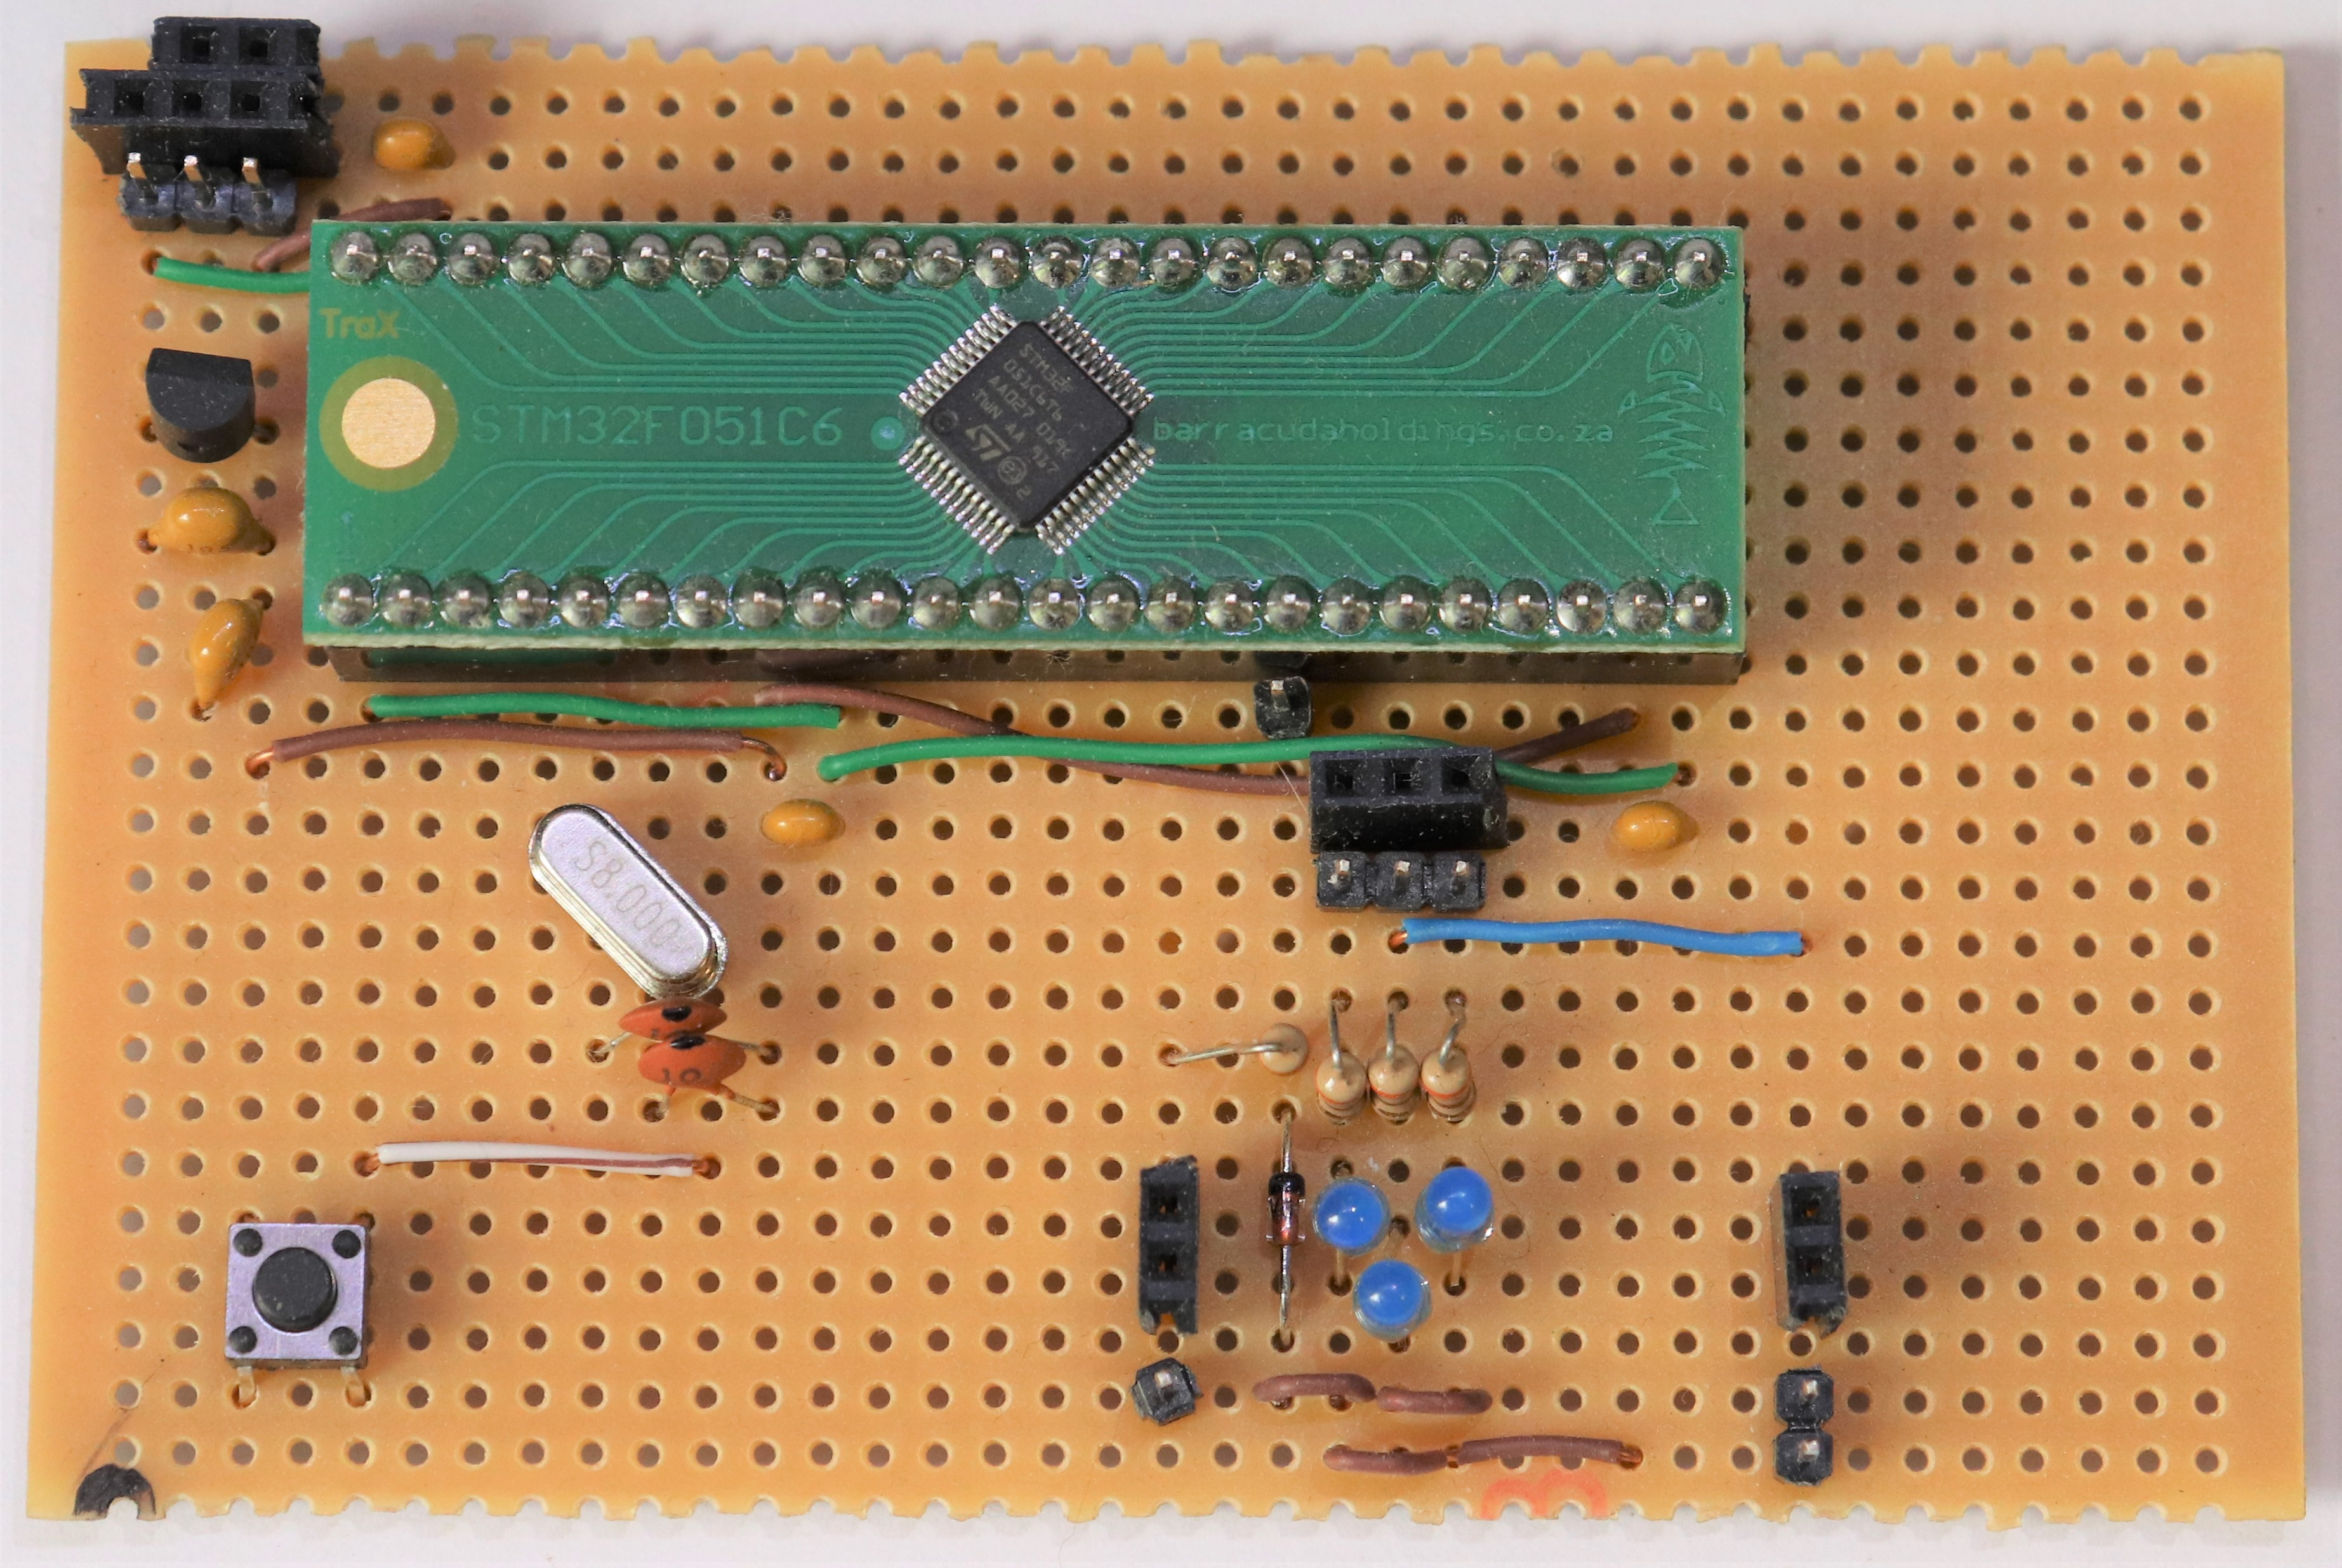
\includegraphics[width=.6\textwidth]{figures/modules/goertzel_filter.jpg}
	\caption{Tone Decoder Module}
	\label{fig:module_tone_decoder}
\end{figure}




%%%%%%%%%%%%%%%%%%%%%%%%%%%%%%%%%%%%%%%%%%%%%%%%%%%%%%%%%%%
%%%%%%%%%%%%%%%%%%%%%%%%%%%%%%%%%%%%%%%%%%%%%%%%%%%%%%%%%%%



\section{Software Design}

\subsection{Tone Decoder Software}
\label{tone_decoder_software}

In section \ref{sec:goertzel_implementation} the goertzel algorithm is given. The parameters k (the DFT frequency bin) and N (the number of samples per frequency bin coefficient calculation) determine the value of omega which in turn affects the value of 'cosval', 'sinval' and 'coeff'. The value of k is also affected by the ratio of the frequency of the k\textsuperscript{th} DFT frequency bin to the sampling frequency (f\textsubscript{sampling}).

The STM32F0 is designed to be low cost 32-bit microcontroller and utilizes the ARM Cortex-M0 CPU core. To reduce costs, this microcontroller does not contain any dedicated DSP peripherals nor does it contain any hardware dedicated to floating point arithmetic. Therefore careful consideration must be taken during design to optimize the performance of the goertzel filter implementation. The STM32F0 is equipped with several timers, a DMA peripheral and an advanced interrupt controller, these peripherals are indispensable for the implementation of the real-time digital filter. Figure \ref{fig:goertzel_functional_diagram} shows the functional blocks for the goertzel filter, the flow of data and clock signals.

\begin{figure}[H]
	\centering
	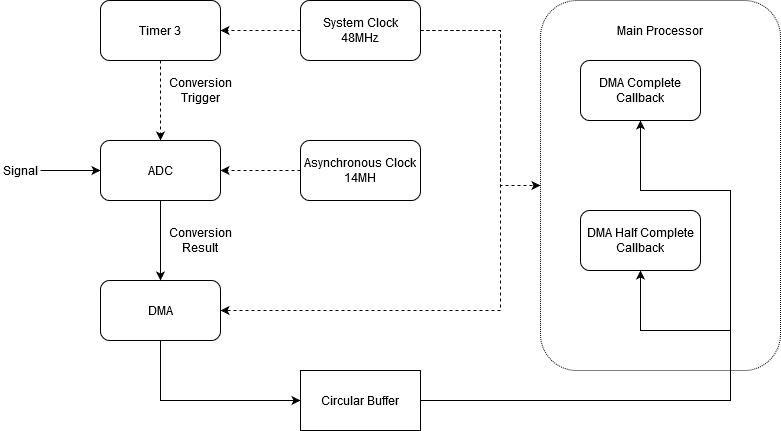
\includegraphics[width=.8\textwidth]{figures/design/goertzel_filter_functional.png}
	\caption{Goertzel Filter Functional Block Diagram}
	\label{fig:goertzel_functional_diagram}
\end{figure}

\subsubsection{Sampling Frequency Constraints}
\label{sec:sampling_frequency_constraints}
The sampling frequency determines the highest frequency that may be present in the sampled waveform before aliasing will occur. The higher the sampling rate, the wider the bandwidth of the goertzel filter. A higher sampling frequency also results in relaxed requirements for the antialiasing filter.

The sampling frequency is limited however by the speed of the microcontroller. This limitation influences the sampling frequency directly by acting as an upper bound to the rate at which the ADC can process and store each analog reading, however more critically, the sampling frequency is directly proportional to the number of samples that must be processed per period. Therefore it is necessary to keep the sampling frequency as low as possible.

\subsubsection{Filter Optimization}
\label{sec:filter_optimization_design}
As outlined at the beginning of this section, the most critical means of optimization for this filter is the full utilization of available peripherals. After reset, the main processor configures the timer, ADC and DMA to continuously sample the incoming signal and store the conversion results in a circular buffer. After this configuration, the main processor is freed from this process and all processing cycles are dedicated to processing the data being stored in the circular buffer.

The second means of optimization was realised after examination of the goertzel algorithm. By carefully engineering the configurable parameters in the goertzel algorithm (listing \ref{lst:goertzel_algorithm}) it is possible to reduce the computation time of the algorithm by removing the multiplication requirement for each new sample (line 13). This is achieved be choosing parameters that result in omega having a value of \(\frac{\pi}{2} + 2\pi m,\; m\epsilon \mathbb{Z}\) and as a consequence make 'cosval' and 'coeff' equal to zero.

It is important to note, this optimization does not improve the time complexity of the algorithm, in both cases the algorithm has a time complexity of O(N). However for real-time algorithms such as in the case of a goertzel filter, every possibly time saving is valuable and can be the difference between a working and failed implementation.

Line 4 of the algorithm provides the relationship between k, N and $\omega$

\begin{equation}
	\omega = \frac{2\pi * k}{N}
\end{equation}

Substituting \(\omega = \frac{\pi}{2} + 2\pi m,\; m\epsilon \mathbb{Z}\) and simplifying shows

\begin{equation}
\label{eqn:k_N_constraint}
	\frac{k}{N} = \frac{1+4m}{4},\; m\epsilon \mathbb{Z}
\end{equation}

If only integer values for k, N, $f_{sampling}$ and $f_{bin}$ are considered, line 3 of the algorithm provides the relationship between these parameters which may be expressed by the following equation

\begin{equation}
\label{eqn:k_N_and_fb_fs}
	\frac{k}{N} = \frac{f_{bin}}{f_{sampling}}
\end{equation}


Equation \ref{eqn:k_N_and_fb_fs} shows that the ratio of $f_{bin}$ to $f_{sampling}$ must be equal to that of k to N. This relationship reveals that the only realisable value for m is zero. Any value of m greater than zero requires a sampling frequency lower than the bin frequency which violates the Nyquist criteria and a negative value of m would require (for $f_{bin} \approx 36kHz$) a negative sampling frequency which is nonsensical. Therefore the final relationship between the ratios may be summarised in the following equation

\begin{equation}
\label{eqn:k_N_and_fb_fs_ratio}
\frac{k}{N} = \frac{f_{bin}}{f_{sampling}} = \frac{1}{4}
\end{equation}

Even after the above two means of optimizing the goertzel algorithm, the STM32F0 was not fast enough to process every sample. This is because even after optimizing the algorithm, it cannot processing incoming samples faster than the required 144kHz. The solution is to sample more than N samples per interrupt and drop the excess samples. This increases the amount of processing time per sample, but increases the latency between the filter's input and the output. This technique only works if the duration of modulation is much greater than the duration of samples dropped.

\subsubsection{Practical Implementation}

The desired bin frequency is 36kHz, according to equation \ref{eqn:k_N_and_fb_fs_ratio} this requires a sampling frequency of 144kHz. This is within the constraints set out in section \ref{sec:sampling_frequency_constraints}.

The ADC conversions are triggered by timer 3, a general purpose 16-bit timer. The timer accepts a pre-scalar and counter period value. The frequency of the timer's output and as a result the sampling frequency is given by \(f_{sampling} = \frac{f_{system\_clock}}{prescaler \times cperiod}\). Substituting our system clock frequency, desired sampling frequency and rearranging the equation we find the product of the pre-scalar and clock period values.

\[prescaler \times cperiod = \frac{48 \times 10^6}{144 \times 10^3} = 333.\dot{3}\]

The result, $333.\dot{3}$ cannot be formed as the product of two integer values, instead the closest integer value of 333 is used. Because this is well below the maximum value of the 16-bit counter period register, the pre-scalar is set to one. The resulting sampling frequency is $144.\dot{1}4\dot{4}$ kHz. Returning to equation \ref{eqn:k_N_and_fb_fs_ratio}, we see that we must choose $f_{bin} = 36.036$kHz to preserve the ratio required for optimization.

%todo: smitz trigger and such - did i do that yet??
The output of the Goertzel filter module is a digital state indicating the presence or absence of a 36kHz frequency. It was chosen to let a high output indicate the detection of the carrier frequency while a low output would indicate no detection.

A value of $6\times 10^{6}$ was selected as the threshold for the squared magnitude of the DFT bin's coefficient. A Schmitt-trigger was used to prevent oscillations while the squared magnitude of the coefficient is crossing this threshold. The output was configured to activate when the value exceeds the threshold by $2\times 10^{6}$ and deactivate when the value decreased by $2\times 10^{6}$ below the threshold.

\begin{figure}[H]
	\centering
	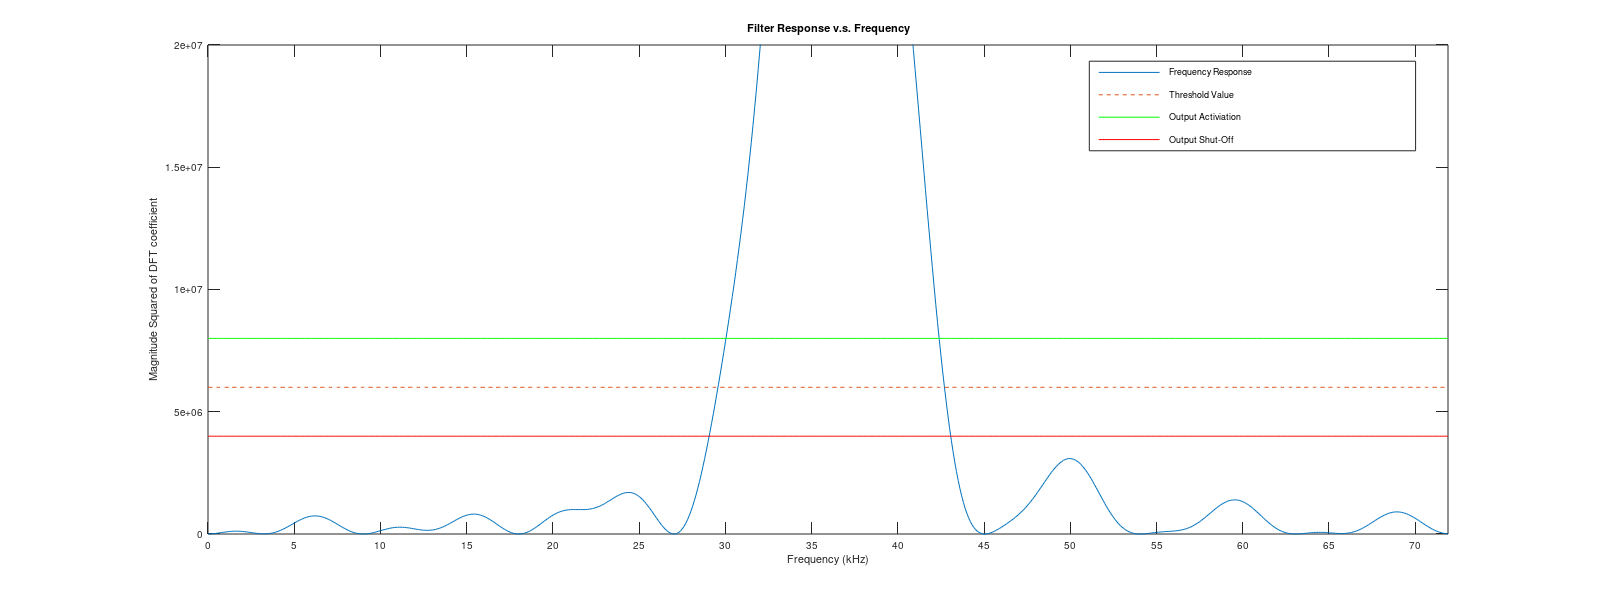
\includegraphics[width=.8\textwidth]{figures/design/schmit_simulation_wide.png}
	\caption{Schmitt Trigger Visualization}
	\label{fig:schmit_simulation_wide}
\end{figure}

Figure \ref{fig:schmit_simulation_wide} illustrates the activation and shut-off boundaries, based on the chosen threshold. The threshold and Schmitt-trigger values were chosen by inspecting the experimental results from the frequency response simulation results (see figure \ref{fig:goertzel_filter_response_simulated}) and selecting values which would allow sensitivity for input signals of differing amplitudes without triggering for side lobes of large amplitude signals.

%todo: ensure I mention improvements to this by using automatic gain control and therefore being able to raise the threshold value




%%%%%%%%%%%%%%%%%%%%%%%%%%%%%%%%%%%%%%%%%%%%%%%%%%%%%%%%%%%



\subsection{Tagger Software}

For the purposes of this investigation, a tagger needed to be created that can encode a gun ID and possibly some additional bits for other information. It was chosen to use a 16-bit packet size. In this initial implementation a single bit is reserved for error detection, however further development of this system might explore the use of hamming codes which would require an additional four bits to be reserved for error correction.

\subsubsection{Modified RC-5 Protocol}
The RC-5 protocol was used as the basis for the design of the modified transmission protocol. A detailed breakdown of the protocol is given in the literature review in section \ref{sec:rc_5_protocol}. In this modified version of the RC-5 protocol, the Manchester Encoding technique and bit-period timing specifications are preserved. However the structure of the bits transmitted has been modified and the period between messages was decreased.

\begin{figure}[H]
	\centering
	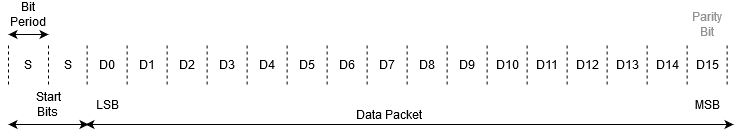
\includegraphics[width=0.8\linewidth]{figures/design/modified_rc5_protocol.png}
	\caption{Modified Bit Structure of RC-5 IR Protocol}
	\label{fig:modified_rc_5_protocol}
\end{figure}

Figure \ref{fig:modified_rc_5_protocol} shows the modified structure for a single transmission. The two start bits are preserved. Following this, the toggle bit, address bits and command bits have been merged into a single set of data bits with an additional 4 bits having been included to increase the number of bits to 16. In the modified protocol the bit order of has been reversed. It should be noted that data bit D15 is used for the parity checksum.

%todo: ref the experiement below
The original RC-5 protocol specifies a period of 114mS between transmissions, however this gap is longer than necessary and following the experiment performed in section \ref{label} it was determined that this period could be reduced to XXXmS.

\subsubsection{Realization}

The tagger software comprises a set of functions dedicated to the encoding of a 15-bit data packet. Implementation of the Manchester Encoding is done purely using timers and interrupts ensuring precise timing and freeing the main processor loop for handling lower priority tasks such as managing player data.

The following functions relating to the generation of a Manchester waveform on the pre-defined output GPIO pin were created

\begin{lstlisting}[style=cstyle, caption=Transmission Related Functions\label{transmission_related_functions}]
	uint8_t get_parity_15(uint16_t packet); //processes a 15-bit long data packet and returns the even parity
	uint32_t wrap_data_15(uint16_t data); //processes a 15-bit long data packet and returns 18-bit bitstream for transmission
	generate_manchester(uint32_t buffer, uint8_t num_bits); //starts Manchester encoded output generation on the pre-define GPIO based on the provided bitstream
\end{lstlisting}

Using one of the dedicated timer peripherals (timer 17) and interrupts for the process of generating the Manchester encoded output required the use of global variables to track the status of an on-going transmission. The following listing shows the global variables along with a brief descriptor comment.

\begin{lstlisting}[style=cstyle, caption=Transmission Status Tracking Variables\label{lst:transmission_status_tracking_variables}]
	volatile uint32_t bit_stream; //bit-stream to be transmitted
	volatile int bit_index; //index of bit currently being transmitted
	volatile int bit_num_transmit; //number of bits from bit-stream to transmit
	volatile int bit_period; //stores current bit period state (0 - first, 1 - second)
	volatile int fire_in_progress; //global indicator of a transmission in progress
	volatile int manchester_timeout_counter; //counts half bit-periods elapsed since last bit was transmitted
\end{lstlisting}

Using interrupts and global variables opens up the possibility for the data corruption to occur. Although the STM32F0 is inherently a serial processor, the main-loop process (responsible for, among other things, initiating transmissions) and the transmission process (the timer interrupt routine) from a high level execute as parallel processes. Figure \ref{fig:parallel_process_abstraction} illustrates how the operations during transmission may be abstracted as two parallel processes. Therefore it is critical to provide a mechanism to prevent one process from modifying any of the variable given in list \ref{lst:transmission_status_tracking_variables} while another process is using them.

\begin{figure}[H]
	\centering
	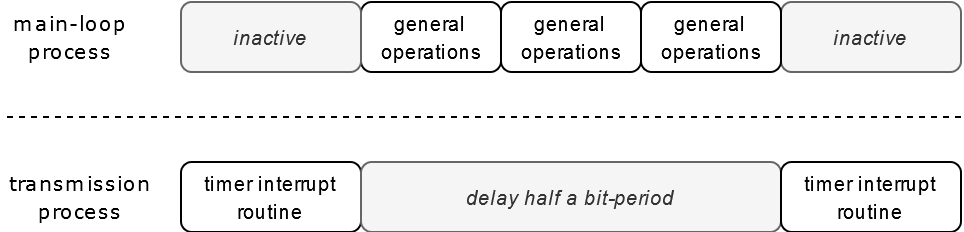
\includegraphics[width=0.8\linewidth]{figures/design/parallel_process_transmission.png}
	\caption{Parallel Process High-Level Abstraction}
	\label{fig:parallel_process_abstraction}
\end{figure}

The purpose of the variable \textit{fire\_in\_progress} is to operate as a synchronization lock. Priority is given to the interrupt process, therefore, in the implementation of the function \textit{generate\_manchester} there is a loop which stalls the processor until any current transmissions complete (see line 4, listing \ref{lst:generate_manchester_implementation}).

Finally, during the transmission process, the logic used to determine the pin state for the purpose of generating the Manchester waveform is given in line 8 of listing \ref{lst:manchester_generate_interrupt_routine}. The pin state for a given half bit-period can be determined as \[pin\_state = \overline{tx\_bit} \;\; \widehat{} \;\; bit\_period\] where tx\_bit is the value of the bit currently being transmitted and bit\_period is as defined in listing \ref{lst:transmission_status_tracking_variables} above.




%%%%%%%%%%%%%%%%%%%%%%%%%%%%%%%%%%%%%%%%%%%%%%%%%%%%%%%%%%%




\subsection{Target Software}

In laser tag it is optimal to have multiple IR detectors placed on various parts of the player. It is therefore important that the tagger software be extendable to process input from multiple input signals simultaneously. To achieve this, the input capture and output compare functions of the STM32 timer peripherals were used. For the purposes of this investigation, the system was developed to only capture a single incoming signal, however the process may be easily expanded to capture multiple incoming signals with little modification.

The target MCU software was separated into four independent processes, these are outlined in figure \ref{fig:target_software_overview} below.

\begin{figure}[H]
	\centering
	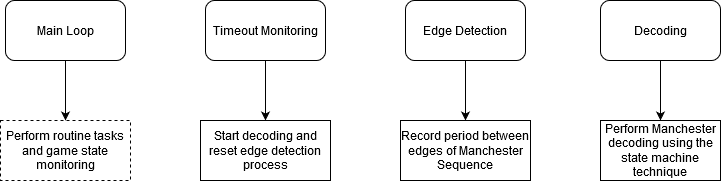
\includegraphics[width=0.8\linewidth]{figures/design/target_software_overview.png}
	\caption{Target MCU Processes}
	\label{fig:target_software_overview}
\end{figure}

The main loop process runs continually and may be used to perform routine tasks.

The edge detection is an interrupt based process which monitors continuously for any rising or falling edges on the input GPIO pin. Each edge is recorded as a time stamp which measures the period elapsed since the previous edge was detected. To reduce unnecessary computation, this value was stored in \textit{ticks} rather than converted into seconds.

The timeout monitoring process is executed by via an interrupt when the output compare register matches the timer's count value. Each time an edge is registered by the edge detection process, the output compare register value is adjusted to allow up to one timeout period before the interrupt is triggered.

The decoding process is an interrupt triggered processes which may also be triggered by software (when the maximum number of edges are recorded). This process decodes the time stamps recorded by the edge detection process and returns the recovered data. The decoding process uses the state machine approach illustrated in figure \ref{fig:manchesterdecodingfsm}.

During the decoding process, the edge detection process responsible for triggering the process is prevented from recording any further edges until the decoding is finished.

\subsubsection{Decoding Strategy}

The state machine approach does not specify an end of transmission condition, therefore it is necessary to define one. It is not possible to simply count the cumulative number of bits as the input capture stage and decoding stages are independent. Therefore a timeout timer will be implemented to trigger the decoding and reset the \textit{array of edge time} differences. In addition to a timeout a maximum number of edges is defined which will also trigger the start of a decoding sequence and reset the state machine.

The timeout period was chosen to be a length of two bit-periods, this was chosen because future inclusion of hamming codes would allow for the correction of a single flipped or missing bit. The timeout period of 3.556ms must be converted into a number of ticks before being used by the output compare functionality of the timer.

\[TIMEOUT\_TICKS = f_{timer} \times T_{timeout} = 8 \times 10^6 \times 3.556 \times 10^{-3} = 28448\]

The maximum number of edges in a valid message occurs when all 16-bits are 1's which results in a Manchester sequence containing 36 edges. Therefore the edge detection process will automatically begin the decoding process if 36 edges are recorded.

The implementation of the Manchester decoding algorithm may be found in the appendix, listing \ref{lst:decode_manchester_implementation}. Decoding requires a time period which defines the difference between a long and short period. This is the \textit{THRESHOLD\_TICKS} constant, in addition a second constant \textit{BITMISS\_TICKS} was defined and is used as a threshold to determine if a bit in the message has been was undetected.










\chapter{Results}
\label{ch_results}

%These are the results I found from my investigation.

%Present your results in a suitable format using tables and graphs where necessary. Remember to refer to them in text and caption them properly.


\section{Simulation Results}


\section{Experimental Results}

\subsection{Focal Length of Lens}

The measured focal length of the lens was measured to be 53mm. Figure \ref{fig:focal_length_experiemnt_result} shows the focused point formed after adjusting the lens to 5.3cm above the working surface.

\begin{figure}[H]
	\centering
	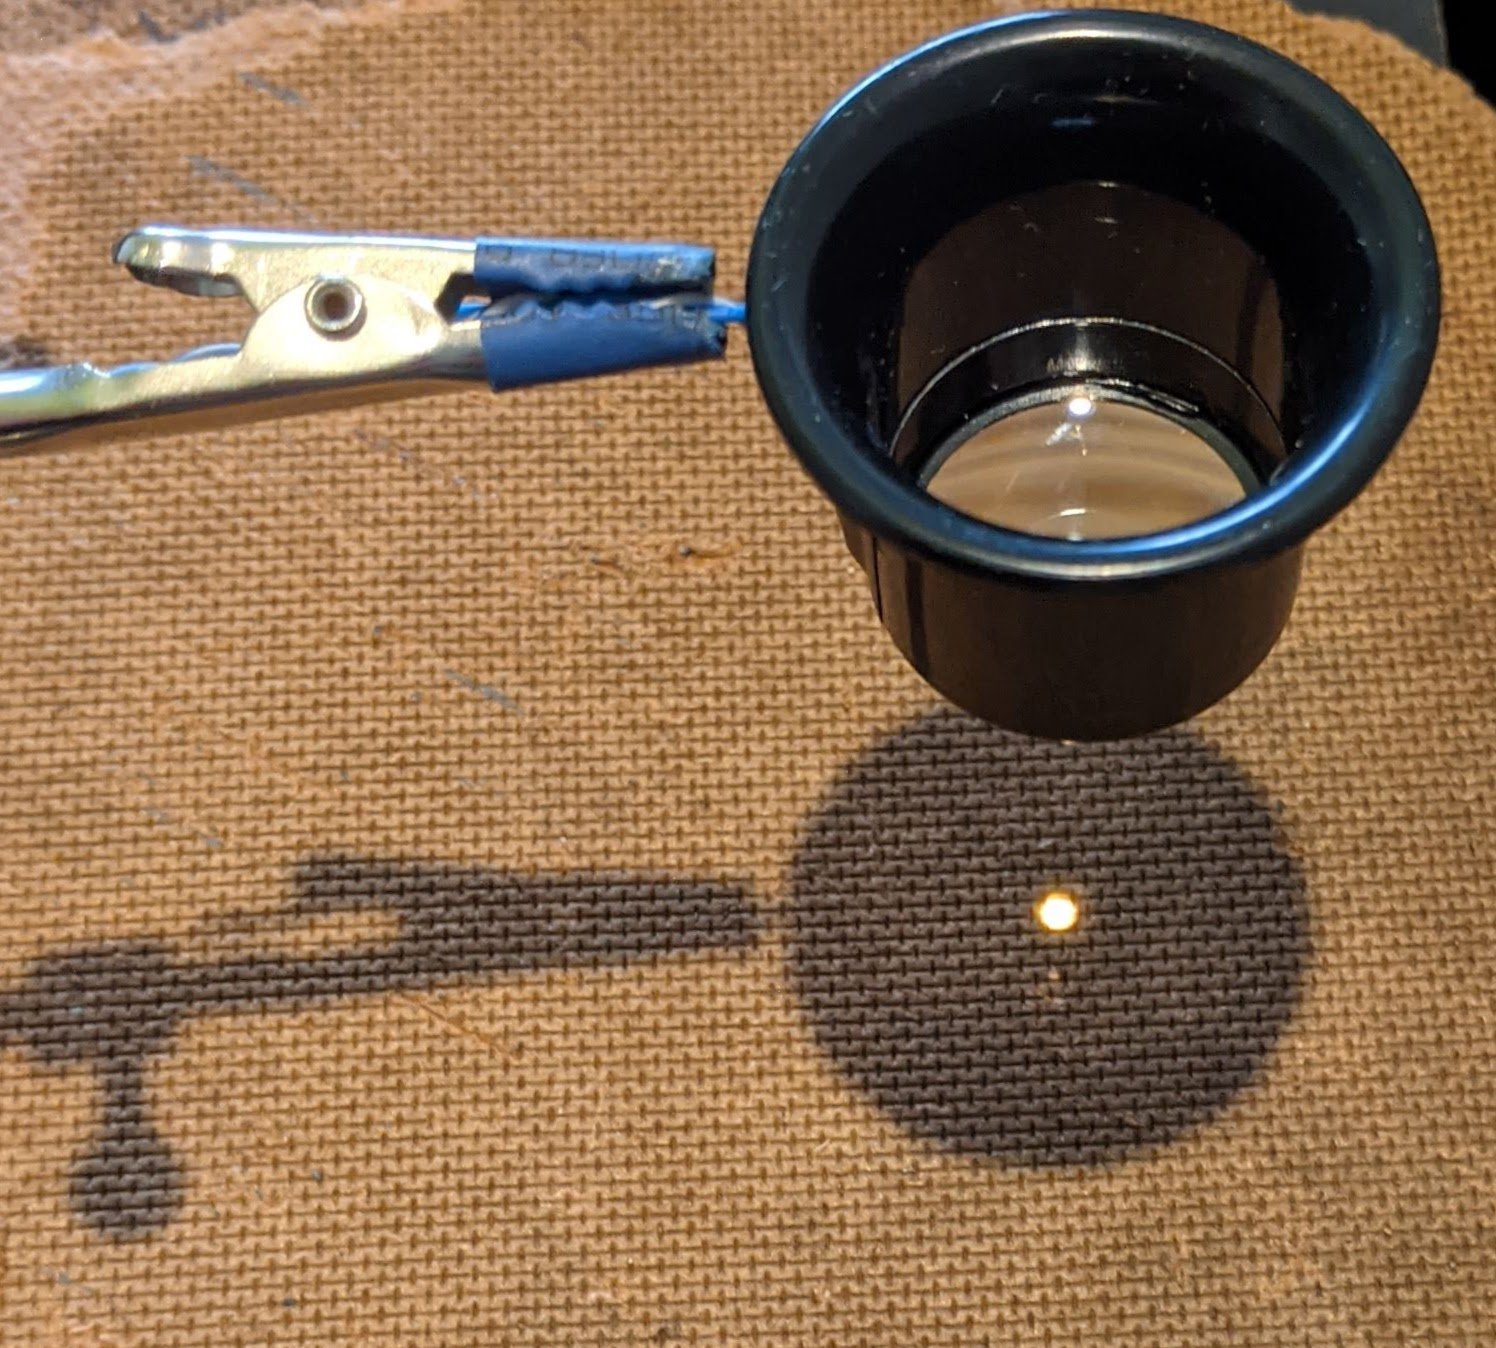
\includegraphics[width=.6\linewidth]{figures/results/focal_length_result.jpg}
	\captionof{figure}{Focal Length Experiemnt}
	\label{fig:focal_length_experiemnt_result}
\end{figure}


\subsection{Light Focus System}

Table \ref{label} below shows the beam spot size vs distance for the IR and warm-white power LEDs.

\begin{figure}[H]
	\centering
	\begin{minipage}{.4\textwidth}
		%todo: make image higher quality after zoom
		\centering
		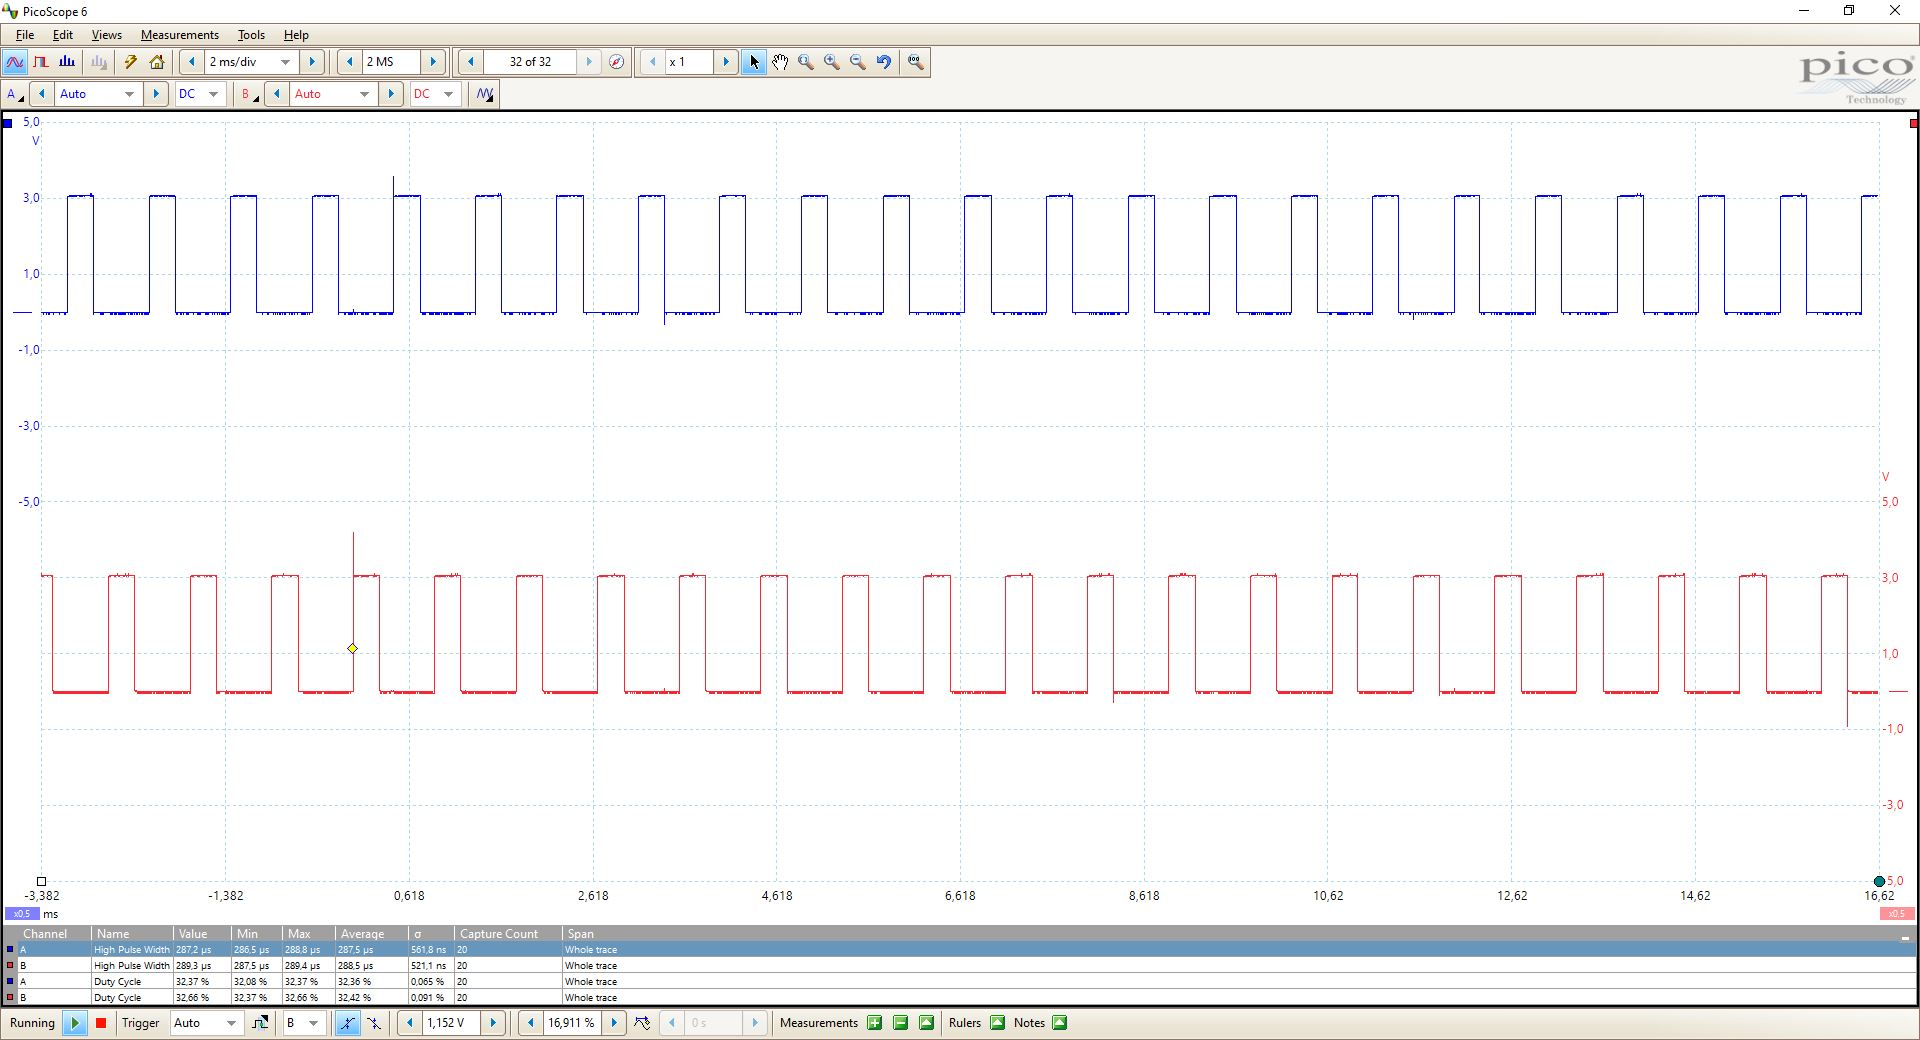
\includegraphics[width=0.9\linewidth]{figures/results/goertzel_filter_speed/16nu.JPG}
		\captionof{figure}{Spot diameter V.S Distance}
		\label{fig:spot_size_vs_distance}
	\end{minipage}%
	\hspace{.1\textwidth}
	\begin{minipage}{.4\textwidth}
		\begin{table}[H]
			\begin{tabular}{cc}
				\hline
				\textbf{\begin{tabular}[c]{@{}c@{}}Distance\\ (m)\end{tabular}} & \textbf{\begin{tabular}[c]{@{}c@{}}Spot Diameter\\ (mm)\end{tabular}} \\ \hline
				1 & 96.46 \\ \hline
				2 & 160.3 \\ \hline
				4 & 287.5 \\ \hline
				8 & 547.2 \\ \hline
				16 & 1059
			\end{tabular}
			\captionof{table}{Tabulation of Spot Diameter V.S. Distance}
			\label{tbl:spot_size_vs_distance}
		\end{table}
	\end{minipage}
\end{figure}

\subsection{Goertzel Filter Optimization}

\begin{figure}[H]
	\centering
	\begin{minipage}{.4\textwidth}
		%todo: make image higher quality after zoom
		\centering
		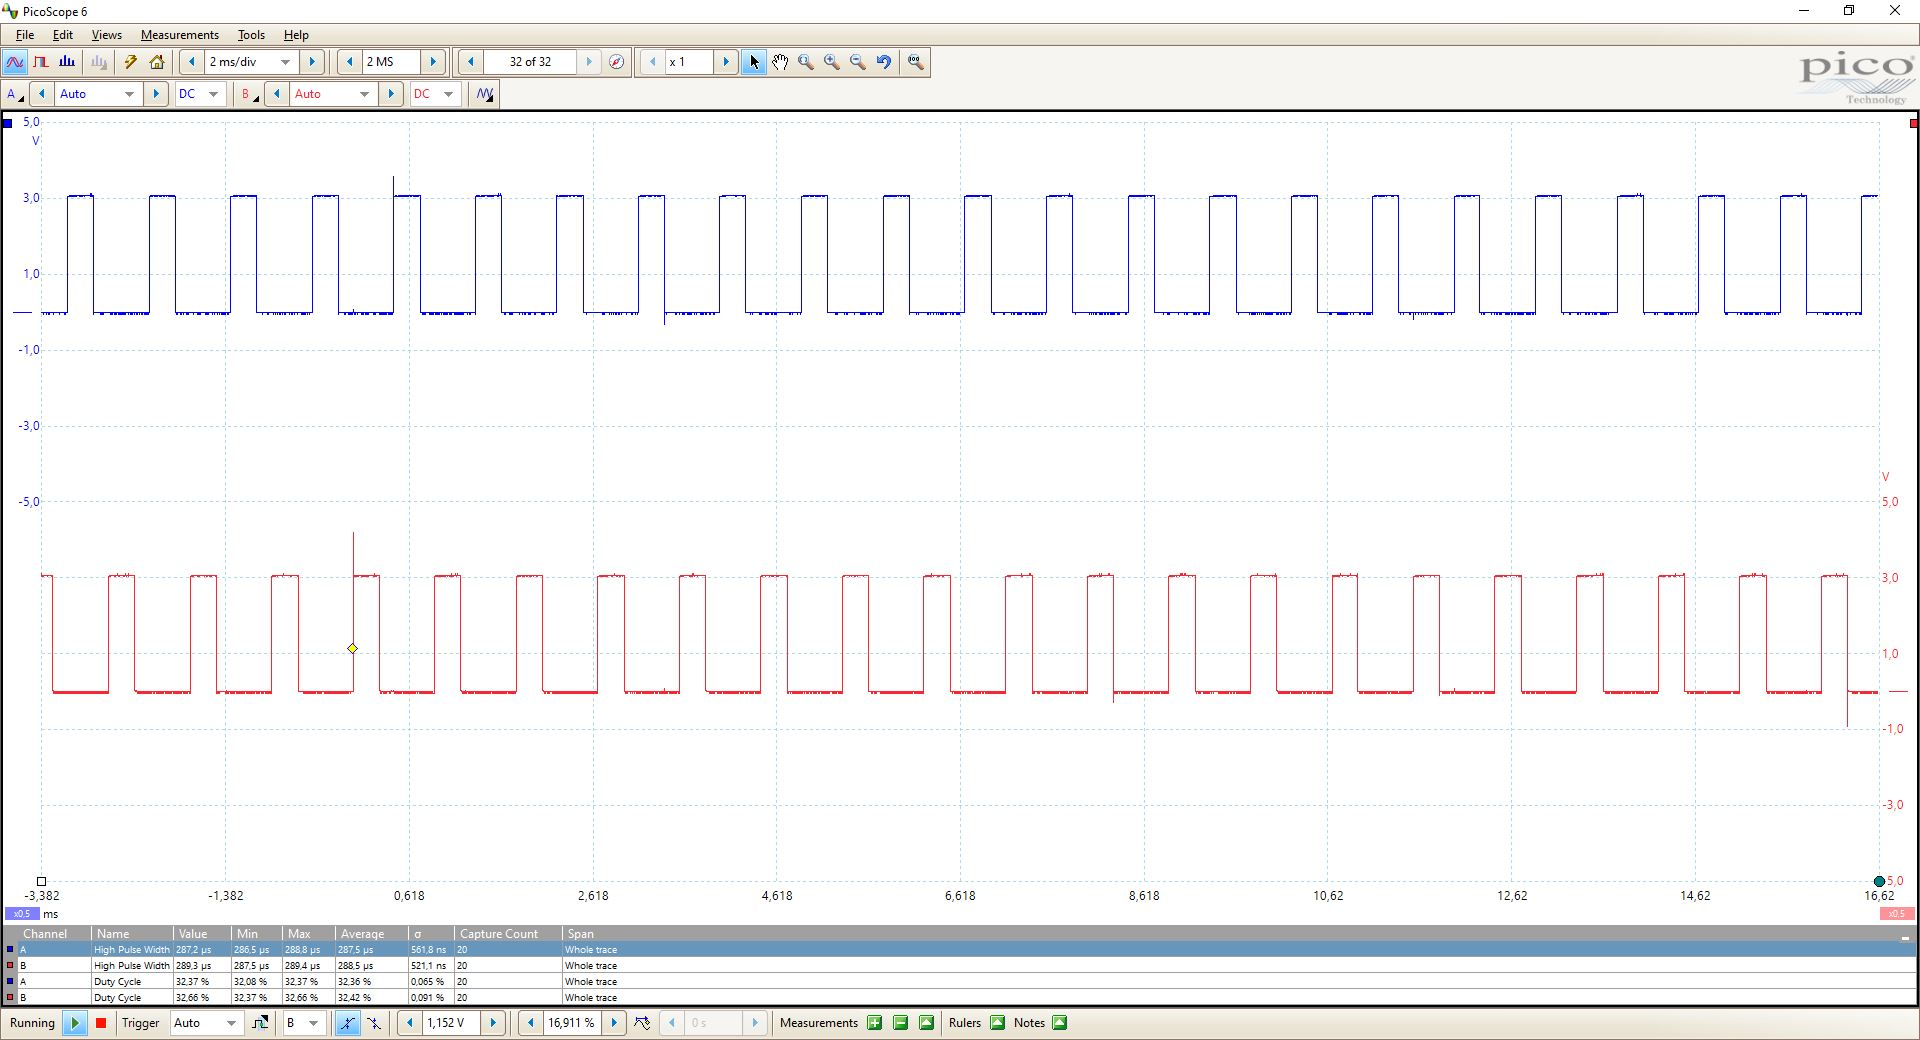
\includegraphics[width=0.9\linewidth]{figures/results/goertzel_filter_speed/16nu.JPG}
		\captionof{figure}{Scope Reading for unoptimized goertzel with $N = 16$}
		\label{fig:goertzel_speed_scope_screenshot}
	\end{minipage}%
	\hspace{.1\textwidth}
	\begin{minipage}{.4\textwidth}
		\begin{table}[H]
			\begin{tabular}{ccc}
				\hline
				\textbf{N} & \textbf{\begin{tabular}[c]{@{}c@{}}Unoptimized\\ ($\mu S$)\end{tabular}} & \textbf{\begin{tabular}[c]{@{}c@{}}Optimized\\ ($\mu S$)\end{tabular}} \\ \hline
				4 & 96.46 & 61.15 \\ \hline
				8 & 160.3 & 98.35 \\ \hline
				16 & 287.5 & 171.9 \\ \hline
				32 & 547.2 & 323.9 \\ \hline
				64 & 1059 & 621.1
			\end{tabular}
			\captionof{table}{Compiled results for goertzel speed experiemnt}
			\label{tbl:goertzel_speed_results}
		\end{table}
	\end{minipage}
\end{figure}

The results from the goertzel algorithm optimization experiment are tabulated in table \ref{tbl:goertzel_speed_results}, the adjacent screenshot shown in figure \ref{fig:goertzel_speed_scope_screenshot} illustrates the output recorded by the oscilloscope software during an iteration of the experiment. The recorded results are plotted in figure \ref{fig:goertzel_computation_plot} to provide graphical insight.

\begin{figure}[H]
	\centering
	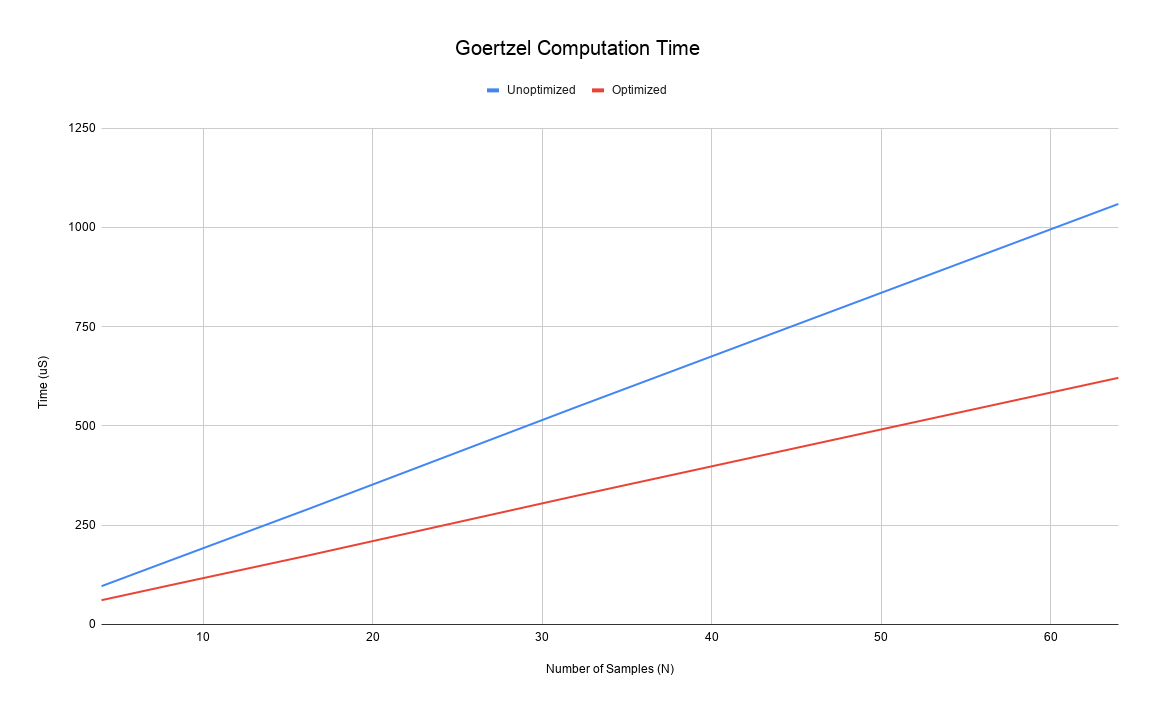
\includegraphics[width=\linewidth]{figures/results/goertzel_filter_speed/goertzel_computation_time.png}
	\captionof{figure}{Goertzel computation time versus sample set size}
	\label{fig:goertzel_computation_plot}
\end{figure}

Figure \ref{fig:goertzel_computation_plot} provides two important insights to the nature of the goertzel algorithm. The first observation may be found in the linearity of both plots, this confirms that both implementations of the algorithm have a time complexity of O(N) as noted in section \ref{sec:filter_optimization_design}. The practically perfect linearity in the results makes it possible to predict the timing requirements and make accurate theoretical predictions.

The gradient of the unoptimized curve is $16\mu S/sample$ and the gradient of the optimized curve is $9.3\mu S/sample$. The sampling rate used was $f_{sampling} \approx 144$kHz or $6.9\mu S/sample$. This indicates that even after optimizing the algorithm by simplifying out the multiplication step required for each new sample, the processor is still not fast enough to keep up with the rate of incoming samples.

The final observation is that the implemented optimization has two implications for the algorithms performance. The first implication is a small but non-zero constant timer saving, this comes as a result of removing the need for the multiplications to find the real and imaginary components of the k\textsubscript{th} DFT coefficient (see lines 18 and 19 of listing \ref{lst:goertzel_algorithm}). The second implication is a time difference which is directly proportional to the number of samples N, as indicated by the different gradients highlighted in the above paragraph.

\subsection{Goertzel Filter Performance}

\subsubsection{Simulated Frequency Response}

The simulation results shown in figure \ref{fig:goertzel_filter_response_simulated} reveal the familiar sinc function embedded in the frequency response curves. The form of these curves can be characterised by the $sinc^2(x)$ function which is to be expected because the filter returns the square of the magnitude.

\begin{figure}[H]
	\centering
	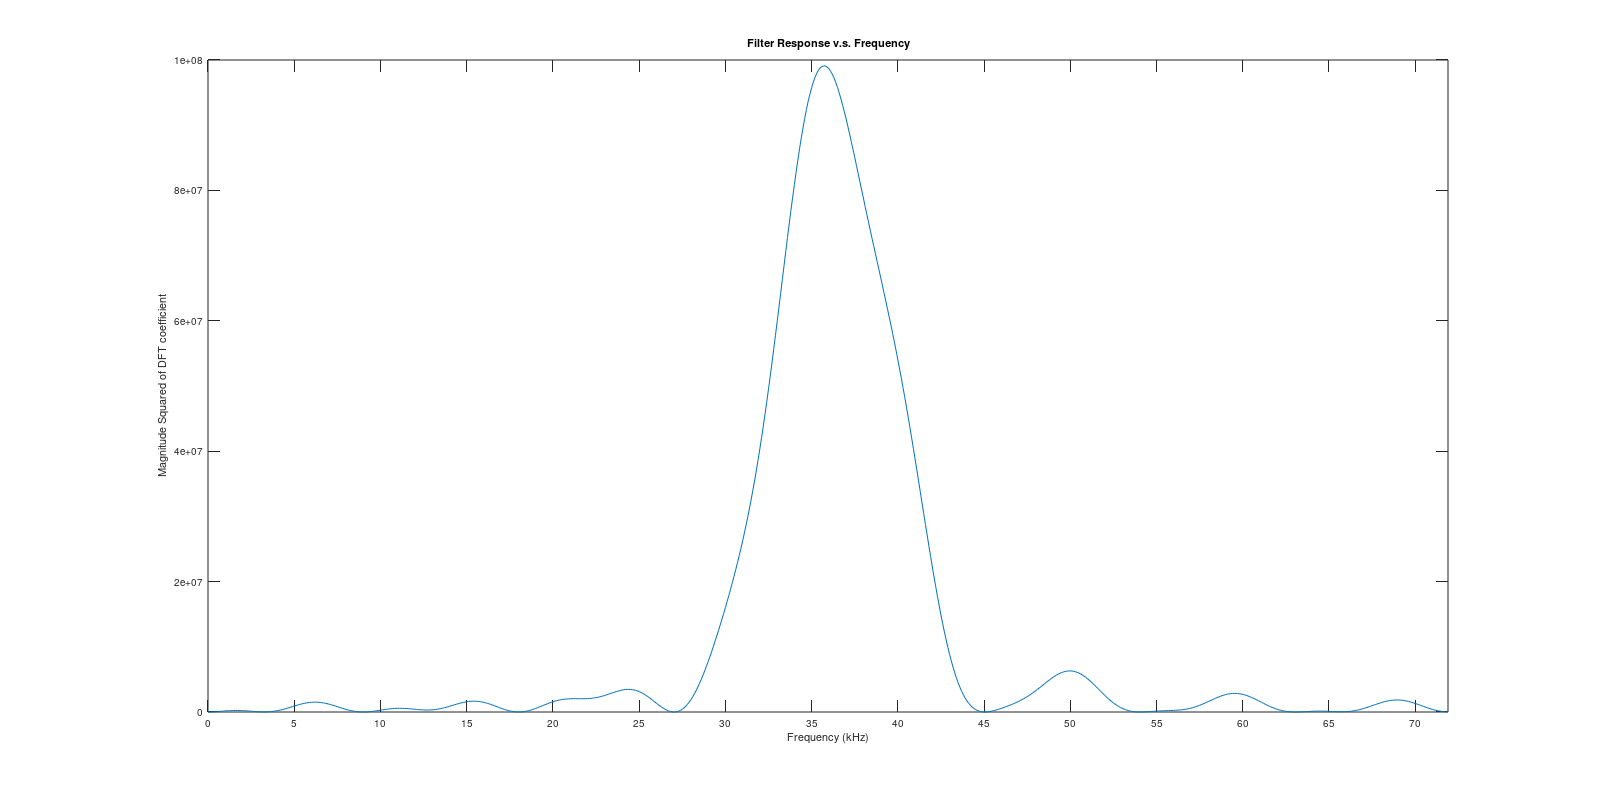
\includegraphics[width=\linewidth]{figures/results/goertzel_filter_simulation_wide.png}
	\caption{Expected Frequency Response - Goertzel Filter}
	\label{fig:goertzel_filter_response_simulated}
\end{figure}

It is clear from the plot that the filter is highly sensitive to the magnitude of the sampled waveform. A decrease in amplitude by a factor of two results in a four fold decrease in the amplitude of the filters response.

%todo: from here onwards I need to write an analysis of results

\subsubsection{Measured Frequency Response}

The following plot in figure \ref{fig:goertzel_filter_response_empirical} show the values returned by the Goertzel filter module and shows the expected frequency response curve.

\begin{figure}[H]
	\centering
	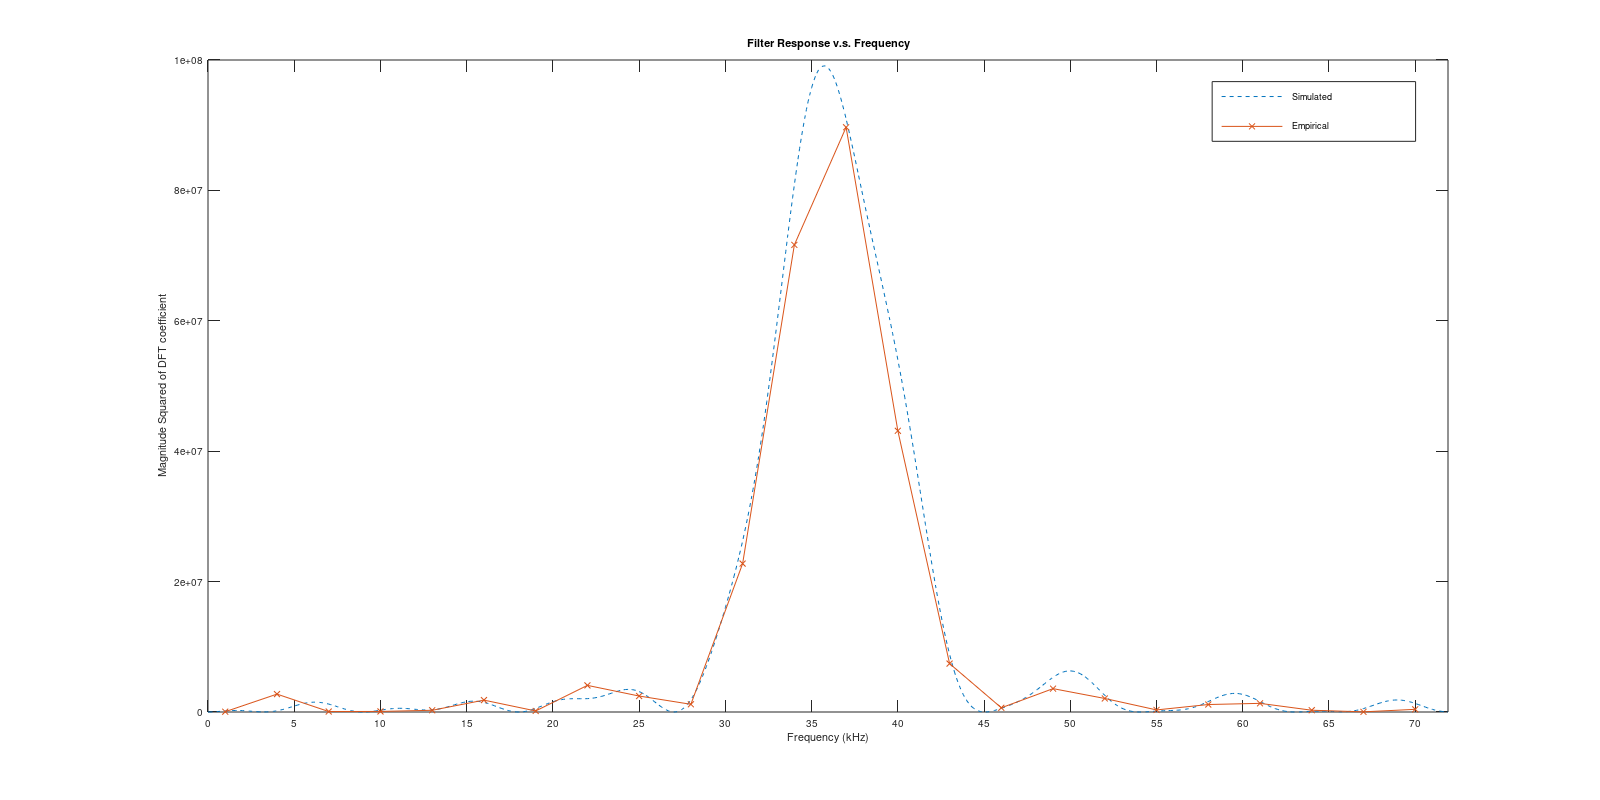
\includegraphics[width=\linewidth]{figures/results/goertzel_filter_empirical_wide.png}
	\caption{Measured Frequency Response - Goertzel Filter}
	\label{fig:goertzel_filter_response_empirical}
\end{figure}


\subsection{Power LED Driver}

The following screenshots shown in figures \ref{fig:pwr_led_6k} through \ref{fig:pwr_led_96k} show the results captured by the oscilloscope. The red trace shows the output of the function generator and the blue trace shows the voltage across the shunt resistor R1\footnote{see schematic in figure \ref{fig:schematic_power_led_driver}}.

\begin{figure}[H]
	\centering
	\begin{minipage}{.399\linewidth}
		\centering
		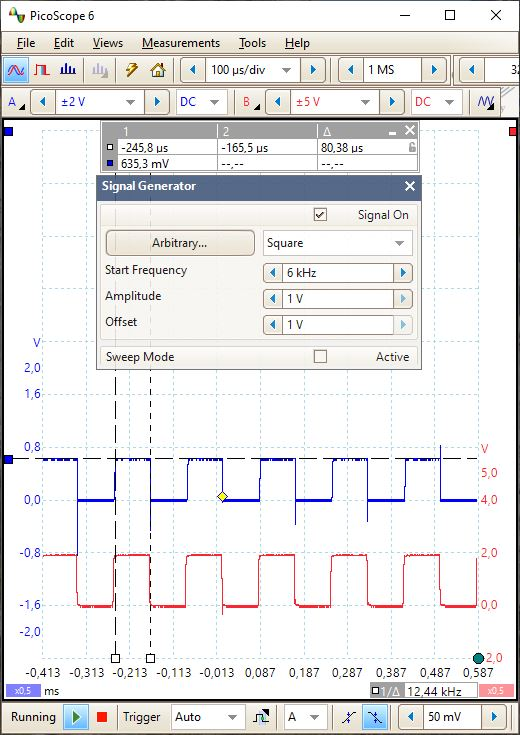
\includegraphics[width=\textwidth]{figures/results/power_led_driver/6khz.JPG}
		\captionof{figure}{6kHz Driving Frequency}
		\label{fig:pwr_led_6k}
	\end{minipage}%
	\hspace{.1\linewidth}
	\begin{minipage}{.399\linewidth}
		\centering
		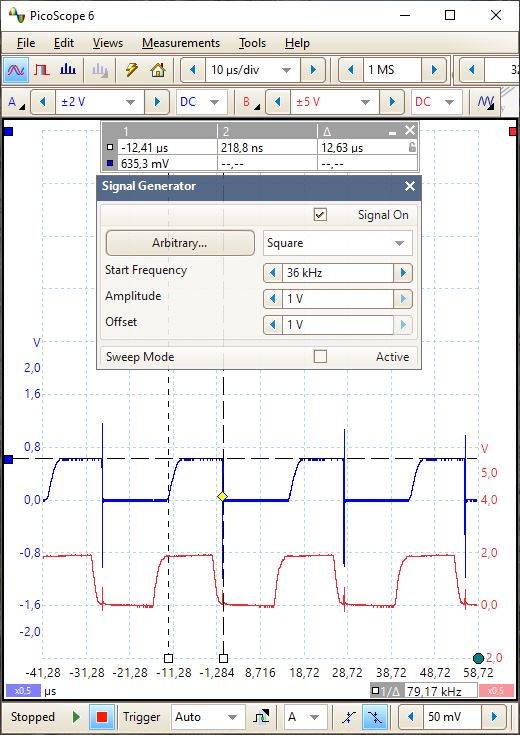
\includegraphics[width=\textwidth]{figures/results/power_led_driver/36khz.JPG}
		\captionof{figure}{36kHz Driving Frequency}
		\label{fig:pwr_led_36k}
	\end{minipage}
\end{figure}

\begin{figure}[H]
	\centering
	\begin{minipage}{.4\linewidth}
		\centering
		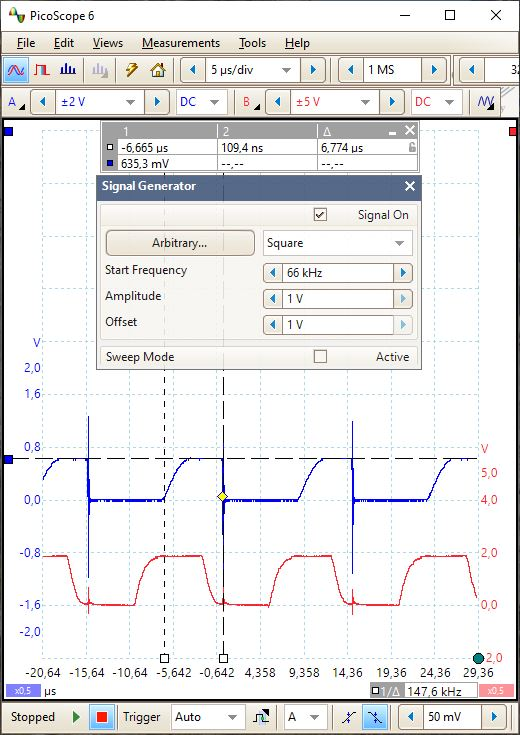
\includegraphics[width=\textwidth]{figures/results/power_led_driver/66khz.JPG}
		\captionof{figure}{66kHz Driving Frequency}
		\label{fig:pwr_led_66k}
	\end{minipage}
	\hspace{.1\linewidth}
	\begin{minipage}{.4\linewidth}
		\centering
		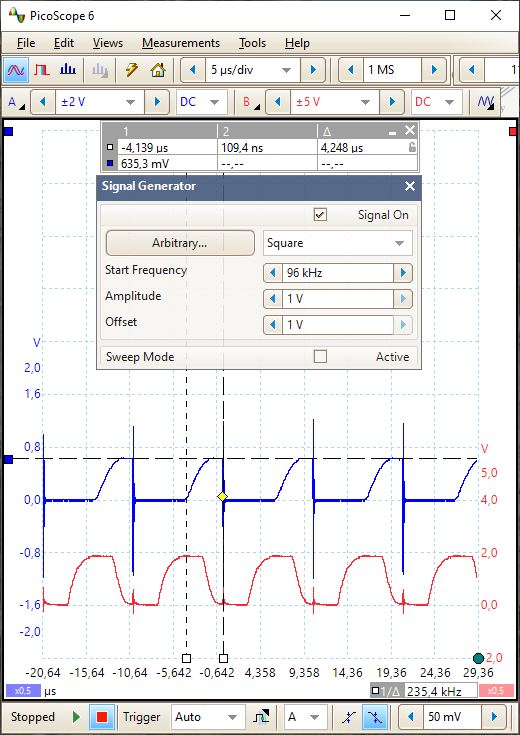
\includegraphics[width=\textwidth]{figures/results/power_led_driver/96khz.JPG}
		\captionof{figure}{96kHz Driving Frequency}
		\label{fig:pwr_led_96k}
	\end{minipage}
\end{figure}

\begin{table}[H]
	\centering
	\begin{tabular}{ccc}
		\hline
		\textbf{\begin{tabular}[c]{@{}c@{}}Frequency\\ (kHz)\end{tabular}} & \textbf{\begin{tabular}[c]{@{}c@{}}LED Current\\ (mA)\end{tabular}} & \textbf{\begin{tabular}[c]{@{}c@{}}Duty Cycle\\ (\%)\end{tabular}} \\ \hline
		6 & 908 & 48.2 \\ \hline
		36 & 908 & 45.5 \\ \hline
		66 & 908 & 44.7 \\ \hline
		96 & 908 & 40.8 \\ \hline
	\end{tabular}
	\caption{Frequency V.S. Current and Pulse Width}
	\label{tbl:led_driver_tabulated_results}
\end{table}



\subsection{Detector Module Directivity}

%todo: make these graphs more bold and readable

\begin{figure}[H]
	\centering
	\begin{minipage}{.4\linewidth}
		\centering
		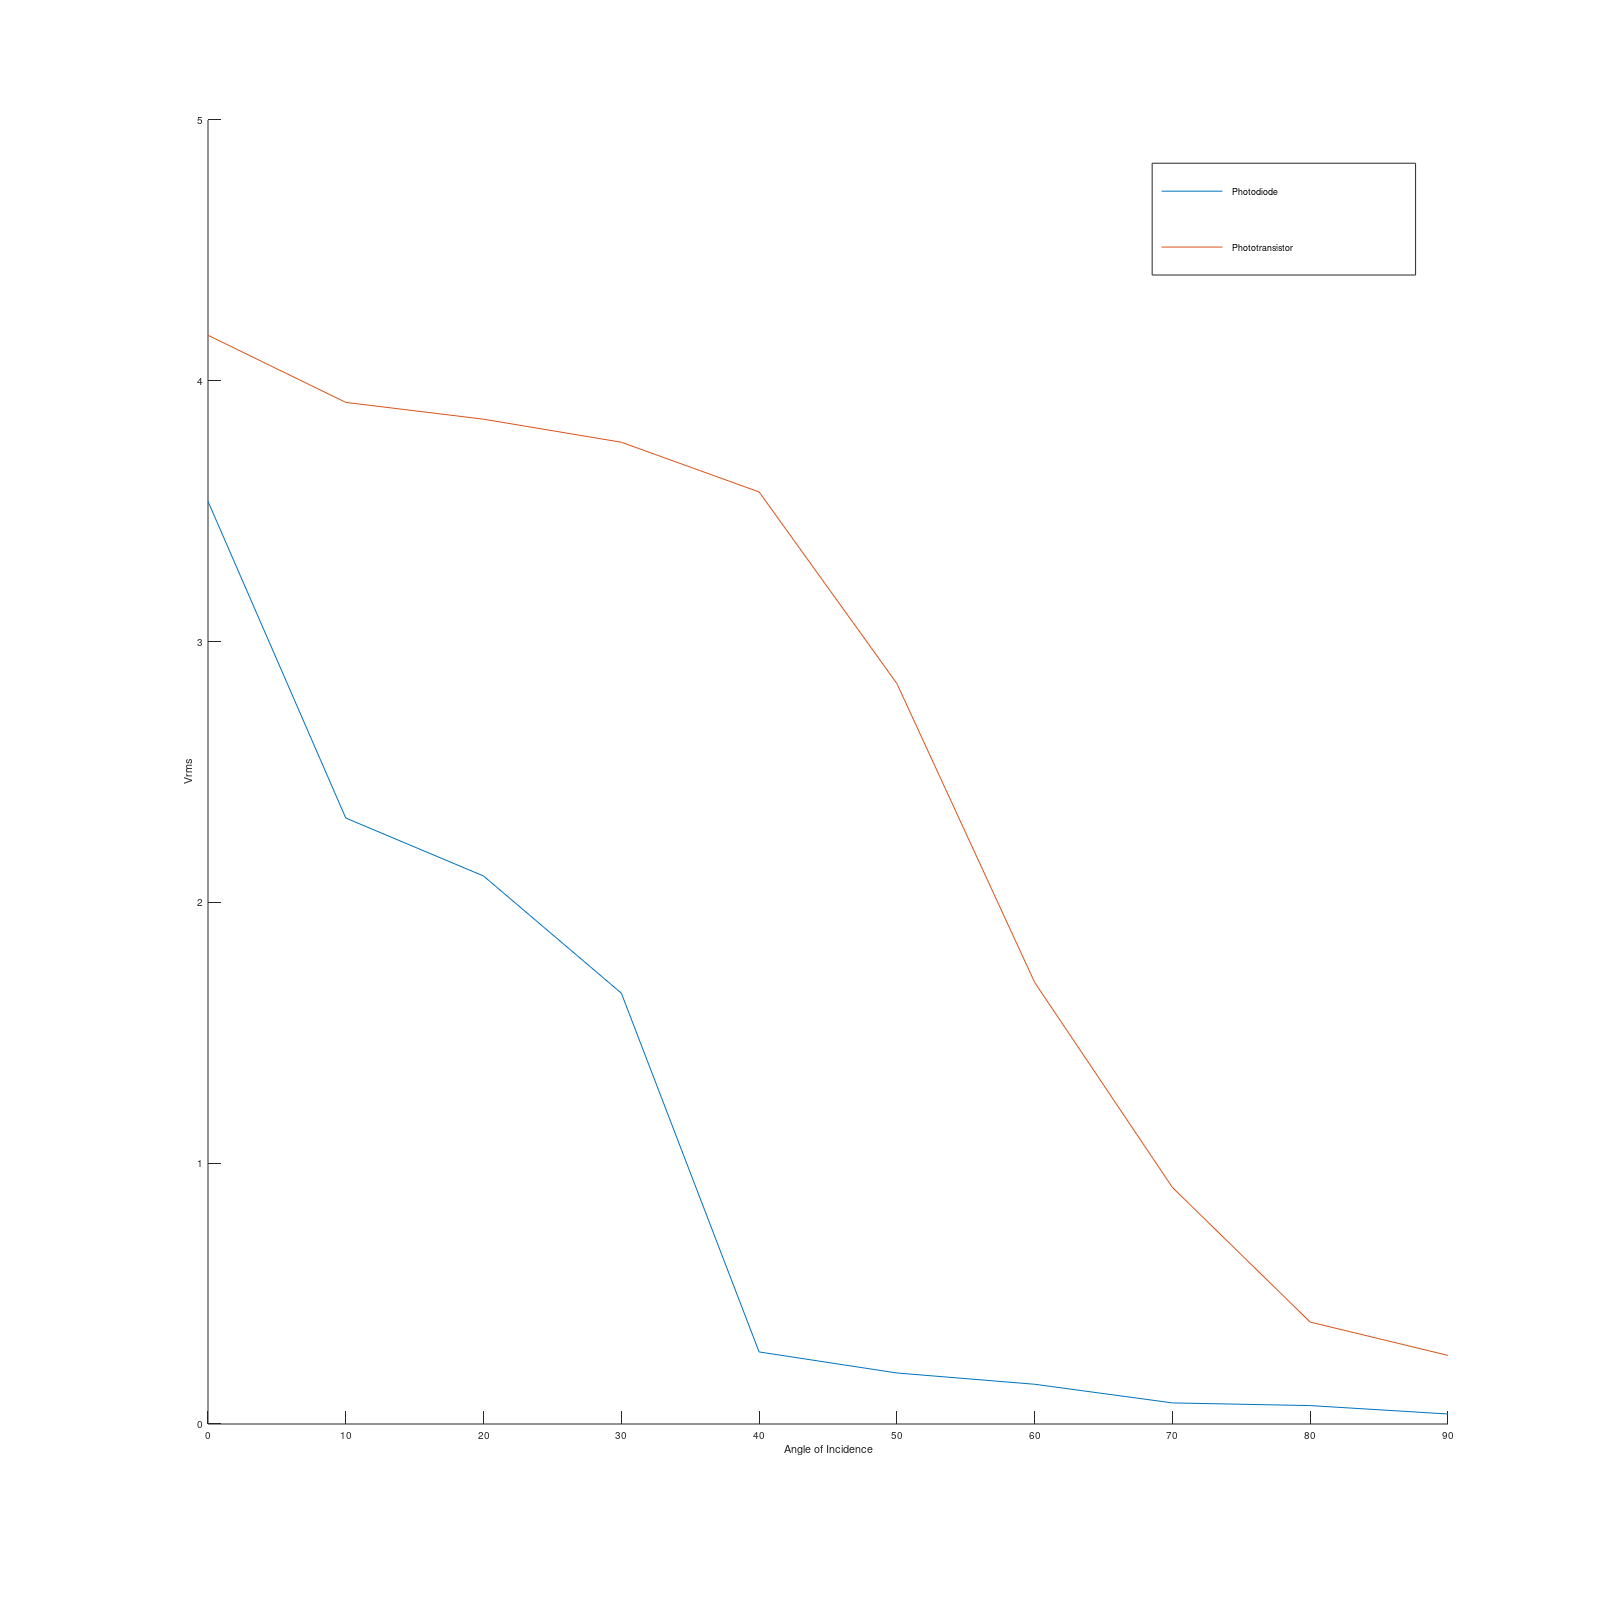
\includegraphics[width=\textwidth]{figures/results/vrms_vs_incidence_square.png}
		\captionof{figure}{Vrms vs Angle of Incidence}
		\label{fig:vrms_vs_angle_of_incidence}
	\end{minipage}
	\hspace{.1\linewidth}
	\begin{minipage}{.4\linewidth}
		\centering
		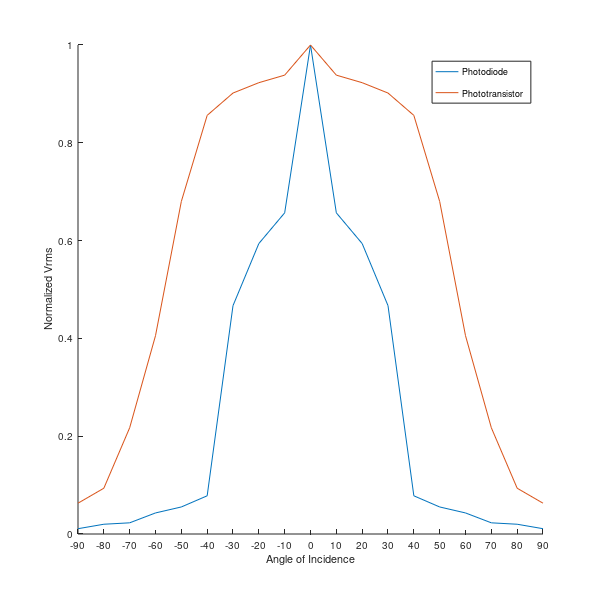
\includegraphics[width=\textwidth]{figures/results/beam_pattern_square.png}
		\captionof{figure}{Beam Pattern}
		\label{fig:beam_pattern}
	\end{minipage}
\end{figure}

\chapter{Discussion}
\label{ch_discussion}
%Here is what the results mean and how they tie to existing literature...
%Discuss the relevance of your results and how they fit into the theoretical work you described in your literature review.


\subsection{Focal Length of Lens}


\subsection{Light Focus System}


\subsection{Goertzel Filter Optimization}

Figure \ref{fig:goertzel_computation_plot} provides two important insights to the nature of the goertzel algorithm. The first observation may be found in the linearity of both plots, this confirms that both implementations of the algorithm have a time complexity of O(N) as noted in section \ref{sec:filter_optimization_design}. The practically perfect linearity in the results makes it possible to predict the timing requirements and make accurate theoretical predictions.

The gradient of the unoptimized curve is $16\mu S/sample$ and the gradient of the optimized curve is $9.3\mu S/sample$. The sampling rate used was $f_{sampling} \approx 144$kHz or $6.9\mu S/sample$. This indicates that even after optimizing the algorithm by simplifying out the multiplication step required for each new sample, the processor is still not fast enough to keep up with the rate of incoming samples.

The final observation is that the implemented optimization has two implications for the algorithms performance. The first implication is a small but non-zero constant timer saving, this comes as a result of removing the need for the multiplications to find the real and imaginary components of the k\textsubscript{th} DFT coefficient (see lines 18 and 19 of listing \ref{lst:goertzel_algorithm}). The second implication is a time difference which is directly proportional to the number of samples N, as indicated by the different gradients highlighted in the above paragraph.


\subsection{Goertzel Filter Performance}

\subsubsection{Simulated Frequency Response}

The simulation results shown in figure \ref{fig:goertzel_filter_response_simulated} reveal the familiar sinc function embedded in the frequency response curves. The form of these curves can be characterised by the $sinc^2(x)$ function which is to be expected because the filter returns the square of the magnitude.

It is clear from the plot that the filter is highly sensitive to the magnitude of the sampled waveform. A decrease in amplitude by a factor of two results in a four fold decrease in the amplitude of the filters response.




\subsubsection{Measured Frequency Response}


\chapter{Conclusions and Recommendations}
\label{ch_conclusions}

%These are the conclusions from the investigation and how the investigation changes things in this field or contributes to current knowledge...

%Draw suitable and intelligent conclusions from your results and subsequent discussion.

The core objective of this study was to develop a modular tagger-target system to provide insight into the potential for more advanced laser tag systems that are robust to ambient lighting conditions and work over longer distances. In addition to this high-level objective, this investigation set out to design and evaluate each module in the full system to provide a foundation for further research.

\section{Review of Modules}
Following the design, implementation and evaluation of the various modules, they have been categorized into two categories based on their performance. %Those categorized as having excellent performance are those that 

\subsection{Excellent Performance}

\textbf{Light Focus System}\\
The light focus system produced an optimal beam in the context of laser tag. The beam spot diameter at short distances (less than 30m) was less than 1m. This beam angle is the ideal size as it ensures some skill is required to aim the tagger while ensuring it isn't so challenging that it is impossible to make a single shot.

It was noted during the system test that for distances greater than 30m, the diameter of light detectable by the IR detectors was less than the size predicted by the beam dispersion experiment. This effect worked to prevent the tagger from being too easy to aim at distant targets.

\textbf{Power LED Driver}\\
The power LED driver module exhibited great performance. The linear current regulation resulted in very precise control over the timing and introduced very little noise into the system. Also, by using a supply with a voltage close to that of the LED, very little heat was dissipated by the driving circuitry.

\textbf{IR Phototransistor Detector}\\
The IR phototransistor detector outperformed the photodiode detector because the amplification stage was robust to saturation caused by a large DC offset.

\textbf{IR Receiver}\\
The all in one package IR receiver outperformed the other IR detector modules, this was likely due to the built-in automatic gain control stage.

\textbf{Tone Decoder}\\ %todo: I want to talk about the speed of detection, but didn't write about the experiment!!! - perhaps if there is time at the end...
The digital tone decoder module exhibited exemplary performance. The high performance was made possible through the optimized implementation of the Goertzel algorithm. The tone decoder was very quick to detect the presence of a tone and because of the Schmitt-trigger, it provided a stable output.

The tone decoder did not handle small amplitude signals well, however this is due to the absence of some form of gain control and not a problem with the tone decoder's algorithm.

\subsection{Adequate Performance}




%%%%%%%%%%%%%%%%%%%%

\section{Recommendations}

%recomend using a slightly larger lens

%implementing automatic gain control

%a superior microcontroller with DSP capabilities
\chapter{Recommendations}
\label{ch_recommendations}

Make sensible recommendations for further work. \cite{Knight2013}

Use the IEEE numbered reference style for referencing your work as shown in your thesis guidelines.
Please remember that the majority of your referenced work should be from journal articles, technical
reports and books not online sources such as Wikipedia.

\begin{thebibliography}{5}
\bibitem{smt2011} M. S. Tsoeu and M. Braae, ``Control Systems,'' \emph{IEEE}, {\bf vol. 34(3)}, pp. 123-129, 2011.
\bibitem{jct2010} J. C. Tapson, \emph{Instrumentation}, UCT Press, Cape Town, 2010.
\bibitem{jst2020} J. M. Wylie, \emph{stuff}, UCT Press, Cape Town, 2020.
\end{thebibliography}

\appendix
\chapter{Additional Files and Schematics}
\label{ch_appendixa}

%Add any information here that you would like to have in your project but is not necessary in the main
%text. Remember to refer to it in the main text. Separate your appendices based on what they are for
%example. Equation derivations in Appendix A and code in Appendix B etc.

\lstinputlisting[caption={Optimized Goertzel Algorithm - Octave Function\label{lst:optimized_goertzel_algorithm}}]{../goertzel/hc_calculate_goertzel.m}

\lstinputlisting[caption={Frequency Response Test - Octave Script\label{lst:frequency_response_script}}]{../goertzel/test_goertzel.m}
\chapter{Addenda}
\label{ch_addenda}

\section{Ethics Forms}
}
\end{document}
